\documentclass[a4paper]{book}
\usepackage{a4wide}
\usepackage{makeidx}
\usepackage{fancyhdr}
\usepackage{graphicx}
\usepackage{multicol}
\usepackage{float}
\usepackage{textcomp}
\usepackage{alltt}
\usepackage{times}
\usepackage{ifpdf}
\ifpdf
\usepackage[pdftex,
            pagebackref=true,
            colorlinks=true,
            linkcolor=blue,
            unicode
           ]{hyperref}
\else
\usepackage[ps2pdf,
            pagebackref=true,
            colorlinks=true,
            linkcolor=blue,
            unicode
           ]{hyperref}
\usepackage{pspicture}
\fi
\usepackage[utf8]{inputenc}
\usepackage{doxygen}
\makeindex
\setcounter{tocdepth}{3}
\renewcommand{\footrulewidth}{0.4pt}
\begin{document}
\begin{titlepage}
\vspace*{7cm}
\begin{center}
{\Large contour\_\-filtering }\\
\vspace*{1cm}
{\large Generated by Doxygen 1.5.6}\\
\vspace*{0.5cm}
{\small Thu Sep 17 12:52:33 2009}\\
\end{center}
\end{titlepage}
\clearemptydoublepage
\pagenumbering{roman}
\tableofcontents
\clearemptydoublepage
\pagenumbering{arabic}
\chapter{Class Index}
\section{meshmorph Class List}
Here are the classes, structs, unions and interfaces with brief descriptions:\begin{CompactList}
\item\contentsline{section}{{\bf hxa7241\_\-general::Array$<$ TYPE $>$} }{\pageref{classhxa7241__general_1_1Array}}{}
\item\contentsline{section}{{\bf Complex} }{\pageref{structComplex}}{}
\item\contentsline{section}{{\bf Container} }{\pageref{classContainer}}{}
\item\contentsline{section}{{\bf Controls} }{\pageref{classControls}}{}
\item\contentsline{section}{{\bf e\_\-hash} }{\pageref{structe__hash}}{}
\item\contentsline{section}{{\bf Edge} }{\pageref{classEdge}}{}
\item\contentsline{section}{{\bf Energy} }{\pageref{classEnergy}}{}
\item\contentsline{section}{{\bf f\_\-hash} }{\pageref{structf__hash}}{}
\item\contentsline{section}{{\bf Face} }{\pageref{classFace}}{}
\item\contentsline{section}{{\bf face\_\-grp} }{\pageref{structface__grp}}{}
\item\contentsline{section}{{\bf Gain\_\-Schedule} }{\pageref{classGain__Schedule}}{}
\item\contentsline{section}{{\bf Grid} }{\pageref{structGrid}}{}
\item\contentsline{section}{{\bf Intersecting\_\-Faces} }{\pageref{classIntersecting__Faces}}{}
\item\contentsline{section}{{\bf Wm4::Intr\-Segment3Triangle3$<$ Real $>$} }{\pageref{classWm4_1_1IntrSegment3Triangle3}}{}
\item\contentsline{section}{{\bf Wm4::Intr\-Triangle3Cone3$<$ Real $>$} }{\pageref{classWm4_1_1IntrTriangle3Cone3}}{}
\item\contentsline{section}{{\bf Log} }{\pageref{classLog}}{}
\item\contentsline{section}{{\bf Wm4::Math$<$ Real $>$} }{\pageref{classWm4_1_1Math}}{}
\item\contentsline{section}{{\bf Wm4::Matrix3$<$ Real $>$} }{\pageref{classWm4_1_1Matrix3}}{}
\item\contentsline{section}{{\bf Minmax} }{\pageref{structMinmax}}{}
\item\contentsline{section}{{\bf my\_\-ltv} }{\pageref{structmy__ltv}}{}
\item\contentsline{section}{{\bf Nice} }{\pageref{classNice}}{}
\item\contentsline{section}{{\bf Object} }{\pageref{classObject}}{}
\item\contentsline{section}{{\bf hxa7241\_\-graphics::Octree$<$ TYPE $>$} }{\pageref{classhxa7241__graphics_1_1Octree}}{}
\item\contentsline{section}{{\bf Octree\_\-Agent\_\-Face} }{\pageref{classOctree__Agent__Face}}{}
\item\contentsline{section}{{\bf Octree\_\-Visitor\_\-Check\_\-Face} }{\pageref{classOctree__Visitor__Check__Face}}{}
\item\contentsline{section}{{\bf Octree\_\-Visitor\_\-Face} }{\pageref{classOctree__Visitor__Face}}{}
\item\contentsline{section}{{\bf Octree\_\-Visitor\_\-Measure} }{\pageref{classOctree__Visitor__Measure}}{}
\item\contentsline{section}{{\bf Octree\_\-Visitor\_\-Update} }{\pageref{classOctree__Visitor__Update}}{}
\item\contentsline{section}{{\bf hxa7241\_\-graphics::Octree\-Agent$<$ TYPE $>$} }{\pageref{classhxa7241__graphics_1_1OctreeAgent}}{}
\item\contentsline{section}{{\bf hxa7241\_\-graphics::Octree\-Agent\-V} }{\pageref{classhxa7241__graphics_1_1OctreeAgentV}}{}
\item\contentsline{section}{{\bf hxa7241\_\-graphics::Octree\-Bound} }{\pageref{classhxa7241__graphics_1_1OctreeBound}}{}
\item\contentsline{section}{{\bf hxa7241\_\-graphics::Octree\-Branch} }{\pageref{classhxa7241__graphics_1_1OctreeBranch}}{}
\item\contentsline{section}{{\bf hxa7241\_\-graphics::Octree\-Cell} }{\pageref{classhxa7241__graphics_1_1OctreeCell}}{}
\item\contentsline{section}{{\bf hxa7241\_\-graphics::Octree\-Data} }{\pageref{classhxa7241__graphics_1_1OctreeData}}{}
\item\contentsline{section}{{\bf hxa7241\_\-graphics::Octree\-Dimensions} }{\pageref{classhxa7241__graphics_1_1OctreeDimensions}}{}
\item\contentsline{section}{{\bf hxa7241\_\-graphics::Octree\-Leaf} }{\pageref{classhxa7241__graphics_1_1OctreeLeaf}}{}
\item\contentsline{section}{{\bf hxa7241\_\-graphics::Octree\-Root} }{\pageref{classhxa7241__graphics_1_1OctreeRoot}}{}
\item\contentsline{section}{{\bf hxa7241\_\-graphics::Octree\-Visitor$<$ TYPE $>$} }{\pageref{classhxa7241__graphics_1_1OctreeVisitor}}{}
\item\contentsline{section}{{\bf hxa7241\_\-graphics::Octree\-Visitor\-V} }{\pageref{classhxa7241__graphics_1_1OctreeVisitorV}}{}
\item\contentsline{section}{{\bf Wm4::Quaternion$<$ Real $>$} }{\pageref{classWm4_1_1Quaternion}}{}
\item\contentsline{section}{{\bf Wm4::Quaternion$<$ Real $>$::Constraints} }{\pageref{classWm4_1_1Quaternion_1_1Constraints}}{}
\item\contentsline{section}{{\bf Refractory} }{\pageref{classRefractory}}{}
\item\contentsline{section}{{\bf result} }{\pageref{structresult}}{}
\item\contentsline{section}{{\bf Search\_\-Stats} }{\pageref{structSearch__Stats}}{}
\item\contentsline{section}{{\bf State} }{\pageref{classState}}{}
\item\contentsline{section}{{\bf Wm4::System} }{\pageref{classWm4_1_1System}}{}
\item\contentsline{section}{{\bf Wm4::THash\-Set$<$ TKEY $>$} }{\pageref{classWm4_1_1THashSet}}{}
\item\contentsline{section}{{\bf Wm4::THash\-Table$<$ TKEY, TVALUE $>$} }{\pageref{classWm4_1_1THashTable}}{}
\item\contentsline{section}{{\bf Wm4::TMin\-Heap$<$ Generator, Real $>$} }{\pageref{classWm4_1_1TMinHeap}}{}
\item\contentsline{section}{{\bf Wm4::TMin\-Heap\-Record$<$ Generator, Real $>$} }{\pageref{classWm4_1_1TMinHeapRecord}}{}
\item\contentsline{section}{{\bf Wm4::TSmall\-Unordered\-Set$<$ T $>$} }{\pageref{classWm4_1_1TSmallUnorderedSet}}{}
\item\contentsline{section}{{\bf Wm4::TString\-Hash\-Table$<$ TVALUE $>$} }{\pageref{classWm4_1_1TStringHashTable}}{}
\item\contentsline{section}{{\bf Wm4::TTuple$<$ DIMENSION, TYPE $>$} }{\pageref{classWm4_1_1TTuple}}{}
\item\contentsline{section}{{\bf v\_\-hash} }{\pageref{structv__hash}}{}
\item\contentsline{section}{{\bf vector3} }{\pageref{structvector3}}{}
\item\contentsline{section}{{\bf Wm4::Vector3$<$ Real $>$} }{\pageref{classWm4_1_1Vector3}}{}
\item\contentsline{section}{{\bf hxa7241\_\-graphics::Vector3r} }{\pageref{classhxa7241__graphics_1_1Vector3r}}{}
\item\contentsline{section}{{\bf Vertex} }{\pageref{classVertex}}{}
\item\contentsline{section}{{\bf Vertex\_\-Schedule} }{\pageref{classVertex__Schedule}}{}
\item\contentsline{section}{{\bf Virtual\_\-Disp} }{\pageref{classVirtual__Disp}}{}
\end{CompactList}

\chapter{File Index}
\section{File List}
Here is a list of all files with brief descriptions:\begin{CompactList}
\item\contentsline{section}{\hyperlink{container_8cc}{container.cc} }{\pageref{container_8cc}}{}
\item\contentsline{section}{\hyperlink{container_8h}{container.h} }{\pageref{container_8h}}{}
\item\contentsline{section}{\hyperlink{contour_8cc}{contour.cc} }{\pageref{contour_8cc}}{}
\item\contentsline{section}{\hyperlink{contour_8h}{contour.h} }{\pageref{contour_8h}}{}
\item\contentsline{section}{\hyperlink{control__points_8cc}{control\_\-points.cc} }{\pageref{control__points_8cc}}{}
\item\contentsline{section}{\hyperlink{control__points_8h}{control\_\-points.h} }{\pageref{control__points_8h}}{}
\item\contentsline{section}{\hyperlink{controls_8cc}{controls.cc} }{\pageref{controls_8cc}}{}
\item\contentsline{section}{\hyperlink{controls_8h}{controls.h} }{\pageref{controls_8h}}{}
\item\contentsline{section}{\hyperlink{histogram_8cc}{histogram.cc} }{\pageref{histogram_8cc}}{}
\item\contentsline{section}{\hyperlink{histogram_8h}{histogram.h} }{\pageref{histogram_8h}}{}
\item\contentsline{section}{\hyperlink{object_8cc}{object.cc} }{\pageref{object_8cc}}{}
\item\contentsline{section}{\hyperlink{object_8h}{object.h} }{\pageref{object_8h}}{}
\item\contentsline{section}{\hyperlink{parameter_8cc}{parameter.cc} }{\pageref{parameter_8cc}}{}
\item\contentsline{section}{\hyperlink{parameter_8h}{parameter.h} }{\pageref{parameter_8h}}{}
\item\contentsline{section}{\hyperlink{point_8cc}{point.cc} }{\pageref{point_8cc}}{}
\item\contentsline{section}{\hyperlink{point_8h}{point.h} }{\pageref{point_8h}}{}
\item\contentsline{section}{\hyperlink{proximity__energy_8m}{proximity\_\-energy.m} }{\pageref{proximity__energy_8m}}{}
\item\contentsline{section}{\hyperlink{reconstruct2contourtiler_8cc}{reconstruct2contourtiler.cc} }{\pageref{reconstruct2contourtiler_8cc}}{}
\item\contentsline{section}{\hyperlink{reconstruct2contourtiler_8h}{reconstruct2contourtiler.h} }{\pageref{reconstruct2contourtiler_8h}}{}
\item\contentsline{section}{\hyperlink{sim__anneal_8cc}{sim\_\-anneal.cc} }{\pageref{sim__anneal_8cc}}{}
\item\contentsline{section}{\hyperlink{sim__anneal_8h}{sim\_\-anneal.h} }{\pageref{sim__anneal_8h}}{}
\end{CompactList}

\chapter{Class Documentation}
\section{Container Class Reference}
\label{classContainer}\index{Container@{Container}}
{\tt \#include $<$container.h$>$}

Collaboration diagram for Container:\begin{figure}[H]
\begin{center}
\leavevmode
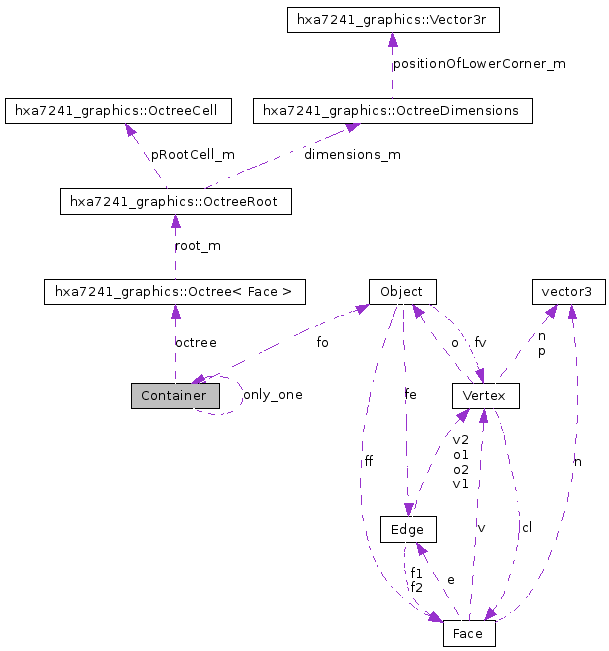
\includegraphics[width=246pt]{classContainer__coll__graph}
\end{center}
\end{figure}
\subsection*{Public Member Functions}
\begin{CompactItemize}
\item 
int {\bf get\-Vertex\-Count} (void) const
\item 
int {\bf get\-Face\-Count} (void) const
\item 
int {\bf get\-Edge\-Count} (void) const
\item 
void {\bf bound\-World} (void)
\item 
void {\bf write\-Summary} (std::ostream \&)
\item 
void {\bf scan\-Dir} (void)
\item 
void {\bf scan\-Files} (void)
\item 
void {\bf assess\-File} ({\bf Object} $\ast$const, char const $\ast$)
\item 
void {\bf scan\-File} ({\bf Object} $\ast$const, char const $\ast$)
\item 
void {\bf compute\-Vertex\-Normals} (void)
\item 
void {\bf create\-Edges} (void)
\item 
void {\bf find\-Vert\-Adj} (void)
\item 
void {\bf read\-Frozen} (char const $\ast$)
\item 
void {\bf sort\-Adjacent\-Faces} (void)
\item 
void {\bf deleteme\_\-check\-Closest\-Face} (int const \&, int const \&, std::string)
\item 
void {\bf check\-Closest\-Face} (int const \&, std::string)
\item 
void {\bf check\-Closest\-Face2} (int const \&, std::string)
\item 
void {\bf check\-Closest\-Face3} (int const \&, std::string)
\item 
void {\bf check\-Faces} (std::string)
\item 
void {\bf check\-Faces\-In\-Octree} (void)
\item 
void {\bf print\-Region\-In\-Octree} (void)
\item 
void {\bf write\-Mesh\-Data} (int const \&) const 
\item 
void {\bf find\-Closest\-Face\-To\-Each\-Vertex} (void)
\item 
void {\bf find\-Closest\-Pt\-In\-Face\-To\-Location} ({\bf vector3} const \&pt, {\bf Face} const $\ast$const face, {\bf vector3} \&p, double \&square\-D) const
\item 
void {\bf find\-Pt\-In\-Face\-Where\-Normal\-Int} ({\bf vector3} const \&pt, {\bf vector3} n, double const \&, {\bf Face} const $\ast$const face, {\bf vector3} \&p, double \&square\-D) const
\item 
bool {\bf face\-Lies\-Opposite\-To\-Normal} ({\bf vector3} const \&, {\bf Face} const $\ast$const face, {\bf vector3} const \&n) const 
\item 
bool {\bf bounding\-Box\-Fully\-In\-Search\-Region} ({\bf vec\_\-d} const \&sr, {\bf vec\_\-d} const \&bb) const
\item 
bool {\bf vertex\-Outside\-Octree\-Bounds} ({\bf vector3} const $\ast$const new\_\-pos)
\item 
bool {\bf closest\-Pt\-Is\-In\-Search\-Cone} ({\bf vector3} const \&pt, {\bf vector3} const \&p, {\bf vector3} const \&n, double const \&) const
\item 
bool {\bf find\-Closest\-Pt\-To\-Barycenter\-Among\-Faces} ({\bf vector3} const \&, {\bf Face} $\ast$const f, {\bf fp\_\-cit}, {\bf fp\_\-cit}, double const \&cone\_\-radius, {\bf vector3} \&, double \&, {\bf Face} $\ast$\&, int \&) const
\item 
bool {\bf find\-Closest\-Pt\-To\-Vertex\-Among\-Faces} ({\bf Vertex} const $\ast$const, {\bf fp\_\-cit}, {\bf fp\_\-cit}, double const \&, {\bf vector3} \&, double \&, {\bf Face} $\ast$\&, int \&) const
\item 
bool {\bf find\-Closest\-Pt\-To\-Vertex} ({\bf Vertex} const $\ast$const, {\bf vector3} \&, double \&, {\bf Face} $\ast$\&) const
\item 
bool {\bf find\-Closest\-Pt\-To\-Barycenter} ({\bf vector3} const \&pt, {\bf Face} $\ast$const f, {\bf vector3} \&, double \&, {\bf Face} $\ast$\&) const
\item 
double {\bf get\-Min\-Edge\-Angle} (void) const
\item 
double {\bf get\-World} (int const \&) const 
\item 
{\bf vec\_\-d} {\bf get\-Spherical\-Cone\-Bounding\-Box} ({\bf vector3} const \&pt, {\bf vector3} n, double const \&cone\_\-radius) const
\item 
{\bf mmap\_\-oi} {\bf load\-Map} (char const $\ast$, {\bf s\_\-set} \&)
\item 
{\bf Object} $\ast$ {\bf get\-Object\-Pointer} (std::string) const 
\item 
std::vector$<$ {\bf Complex} $>$ {\bf load\-Vector} (const char $\ast$filename, {\bf s\_\-set} \&not\_\-found)
\item 
bool {\bf vertex\-Is\-Frozen} ({\bf Vertex} $\ast$const v) const
\item 
int {\bf get\-File\-Count} (void) const
\end{CompactItemize}
\subsection*{Static Public Member Functions}
\begin{CompactItemize}
\item 
static {\bf Container} \& {\bf instance} (void)
\end{CompactItemize}
\subsection*{Public Attributes}
\begin{CompactItemize}
\item 
{\bf hxa7241\_\-graphics::Octree}$<$ {\bf Face} $>$ $\ast$ {\bf octree}
\item 
{\bf vec\_\-o} {\bf o}
\end{CompactItemize}


\subsection{Member Function Documentation}
\index{Container@{Container}!instance@{instance}}
\index{instance@{instance}!Container@{Container}}
\subsubsection{\setlength{\rightskip}{0pt plus 5cm}{\bf Container} \& Container::instance (void)\hspace{0.3cm}{\tt  [static]}}\label{classContainer_e4646d7b418a9b302db245f074ad8ec5}


\index{Container@{Container}!getVertexCount@{getVertexCount}}
\index{getVertexCount@{getVertexCount}!Container@{Container}}
\subsubsection{\setlength{\rightskip}{0pt plus 5cm}int Container::get\-Vertex\-Count (void) const}\label{classContainer_31f05695581593644aafa457cc2b2bc8}


Get the total number of vertices in the input data. \begin{Desc}
\item[Returns:]The total number of vertices in the input data. \end{Desc}
\index{Container@{Container}!getFaceCount@{getFaceCount}}
\index{getFaceCount@{getFaceCount}!Container@{Container}}
\subsubsection{\setlength{\rightskip}{0pt plus 5cm}int Container::get\-Face\-Count (void) const}\label{classContainer_570049d28d9b59a6b314fdbe9978f056}


Get the total number of faces in the input data. \begin{Desc}
\item[Returns:]The total number of faces in the input data. \end{Desc}
\index{Container@{Container}!getEdgeCount@{getEdgeCount}}
\index{getEdgeCount@{getEdgeCount}!Container@{Container}}
\subsubsection{\setlength{\rightskip}{0pt plus 5cm}int Container::get\-Edge\-Count (void) const}\label{classContainer_c805cd419c41dbc672b081b88bcb6552}


Get the total number of edges in the input data. \begin{Desc}
\item[Returns:]The total number of edges in the input data. \end{Desc}
\index{Container@{Container}!boundWorld@{boundWorld}}
\index{boundWorld@{boundWorld}!Container@{Container}}
\subsubsection{\setlength{\rightskip}{0pt plus 5cm}void Container::bound\-World (void)}\label{classContainer_a5fc905c668cc9f7909b9bbcf5beee65}


Calculate and record limits of model along each prinicpal axis. \index{Container@{Container}!writeSummary@{writeSummary}}
\index{writeSummary@{writeSummary}!Container@{Container}}
\subsubsection{\setlength{\rightskip}{0pt plus 5cm}void Container::write\-Summary (std::ostream \& {\em target})}\label{classContainer_a4e9a37eb14178872c1b735aed195eda}


Write description and summary of this class to output stream. \begin{Desc}
\item[Parameters:]
\begin{description}
\item[\mbox{$\leftarrow$} {\em target}]Pre-initialized output stream. \end{description}
\end{Desc}
\index{Container@{Container}!scanDir@{scanDir}}
\index{scanDir@{scanDir}!Container@{Container}}
\subsubsection{\setlength{\rightskip}{0pt plus 5cm}void Container::scan\-Dir (void)}\label{classContainer_e49ee77c3921f10fcc057f61b307251b}


Find all .mesh files in input directory. \index{Container@{Container}!scanFiles@{scanFiles}}
\index{scanFiles@{scanFiles}!Container@{Container}}
\subsubsection{\setlength{\rightskip}{0pt plus 5cm}void Container::scan\-Files (void)}\label{classContainer_d46293c789ebc22aa77b938b85979800}


For each .mesh file found in input directory build an instance of object class.

\begin{Desc}
\item[Returns:]Void. \end{Desc}
\index{Container@{Container}!assessFile@{assessFile}}
\index{assessFile@{assessFile}!Container@{Container}}
\subsubsection{\setlength{\rightskip}{0pt plus 5cm}void Container::assess\-File ({\bf Object} $\ast$ const {\em obj}, char const $\ast$ {\em filename})}\label{classContainer_06befe7555d878137526e7eddd1feec3}


Scan input data file once to count total number of vertices and faces in the object. \begin{Desc}
\item[Parameters:]
\begin{description}
\item[\mbox{$\leftarrow$} {\em obj}]Pointer to parent \doxyref{Object}{p.}{classObject}. \item[\mbox{$\leftarrow$} {\em filename}]Input file name. \end{description}
\end{Desc}
\index{Container@{Container}!scanFile@{scanFile}}
\index{scanFile@{scanFile}!Container@{Container}}
\subsubsection{\setlength{\rightskip}{0pt plus 5cm}void Container::scan\-File ({\bf Object} $\ast$ const {\em obj}, char const $\ast$ {\em filename})}\label{classContainer_1f2ebe727eb7f5d77f77ff9f8e60f339}


Build \doxyref{Object}{p.}{classObject} from input file data. \begin{Desc}
\item[Parameters:]
\begin{description}
\item[\mbox{$\leftarrow$} {\em obj}]Pointer to parent \doxyref{Object}{p.}{classObject}. \item[\mbox{$\leftarrow$} {\em filename}]Input file name. \end{description}
\end{Desc}
\index{Container@{Container}!computeVertexNormals@{computeVertexNormals}}
\index{computeVertexNormals@{computeVertexNormals}!Container@{Container}}
\subsubsection{\setlength{\rightskip}{0pt plus 5cm}void Container::compute\-Vertex\-Normals (void)}\label{classContainer_b103cc06097fab5f1a7204572d7c60c5}


Calculate and record the normal vector of each vertex in the model. \index{Container@{Container}!createEdges@{createEdges}}
\index{createEdges@{createEdges}!Container@{Container}}
\subsubsection{\setlength{\rightskip}{0pt plus 5cm}void Container::create\-Edges (void)}\label{classContainer_4ea77ab7f90acdf56e51e04ddef48808}


For each object build instance of edge class using face and vertex class data. \index{Container@{Container}!findVertAdj@{findVertAdj}}
\index{findVertAdj@{findVertAdj}!Container@{Container}}
\subsubsection{\setlength{\rightskip}{0pt plus 5cm}void Container::find\-Vert\-Adj (void)}\label{classContainer_3406171e70819424f595b04e4c37efc9}


For each vertex in each object add pointers to adjacent faces of vertex to vertex class. \index{Container@{Container}!readFrozen@{readFrozen}}
\index{readFrozen@{readFrozen}!Container@{Container}}
\subsubsection{\setlength{\rightskip}{0pt plus 5cm}void Container::read\-Frozen (char const $\ast$ {\em filename})}\label{classContainer_e63666838eb9afa04f2a54fdec3820f0}


Process frozen vertex data. \begin{Desc}
\item[Parameters:]
\begin{description}
\item[\mbox{$\leftarrow$} {\em filename}]Frozen vertex file name. \end{description}
\end{Desc}
\index{Container@{Container}!sortAdjacentFaces@{sortAdjacentFaces}}
\index{sortAdjacentFaces@{sortAdjacentFaces}!Container@{Container}}
\subsubsection{\setlength{\rightskip}{0pt plus 5cm}void Container::sort\-Adjacent\-Faces (void)}\label{classContainer_a91178ecc1710c316c27f54ed0ede0a9}


Sort adjacent faces of each vertex in model. \index{Container@{Container}!deleteme_checkClosestFace@{deleteme\_\-checkClosestFace}}
\index{deleteme_checkClosestFace@{deleteme\_\-checkClosestFace}!Container@{Container}}
\subsubsection{\setlength{\rightskip}{0pt plus 5cm}void Container::deleteme\_\-check\-Closest\-Face (int const \&, int const \&, std::string)}\label{classContainer_b88ab4f62ffb44dcc2db6650fe405dce}


\index{Container@{Container}!checkClosestFace@{checkClosestFace}}
\index{checkClosestFace@{checkClosestFace}!Container@{Container}}
\subsubsection{\setlength{\rightskip}{0pt plus 5cm}void Container::check\-Closest\-Face (int const \& {\em group}, std::string {\em suffix})}\label{classContainer_5350a46003ff8160b0125a6058c7603c}


Find the closest face of each vertex in container and compare with closest face stored in vertex class.

\begin{Desc}
\item[Parameters:]
\begin{description}
\item[\mbox{$\leftarrow$} {\em group}]Number of group of vertices being moved. \item[\mbox{$\leftarrow$} {\em suffix}]String to append to file name to identify when in the program the file was written. \end{description}
\end{Desc}
\index{Container@{Container}!checkClosestFace2@{checkClosestFace2}}
\index{checkClosestFace2@{checkClosestFace2}!Container@{Container}}
\subsubsection{\setlength{\rightskip}{0pt plus 5cm}void Container::check\-Closest\-Face2 (int const \&, std::string)}\label{classContainer_bebf935e5f2bcbfa593861a88693aa1e}


\index{Container@{Container}!checkClosestFace3@{checkClosestFace3}}
\index{checkClosestFace3@{checkClosestFace3}!Container@{Container}}
\subsubsection{\setlength{\rightskip}{0pt plus 5cm}void Container::check\-Closest\-Face3 (int const \&, std::string)}\label{classContainer_063be9bc92dbc325ac5911550da8a8e9}


\index{Container@{Container}!checkFaces@{checkFaces}}
\index{checkFaces@{checkFaces}!Container@{Container}}
\subsubsection{\setlength{\rightskip}{0pt plus 5cm}void Container::check\-Faces (std::string {\em s})}\label{classContainer_35bf9908f07f7a95a44af9878d41629f}


Check that all faces have flag set to false. \begin{Desc}
\item[Parameters:]
\begin{description}
\item[\mbox{$\leftarrow$} {\em s}]Error message if face found with flag set to true. \end{description}
\end{Desc}
\index{Container@{Container}!checkFacesInOctree@{checkFacesInOctree}}
\index{checkFacesInOctree@{checkFacesInOctree}!Container@{Container}}
\subsubsection{\setlength{\rightskip}{0pt plus 5cm}void Container::check\-Faces\-In\-Octree (void)}\label{classContainer_2b2598775cc2a322fc7ded1d7a54f899}


Check that all faces are present in appropriate octree cells. \index{Container@{Container}!printRegionInOctree@{printRegionInOctree}}
\index{printRegionInOctree@{printRegionInOctree}!Container@{Container}}
\subsubsection{\setlength{\rightskip}{0pt plus 5cm}void Container::print\-Region\-In\-Octree (void)}\label{classContainer_4b1cfa76345dbe77dd8b2b04bb742eee}


Print octree overlapping region. \index{Container@{Container}!writeMeshData@{writeMeshData}}
\index{writeMeshData@{writeMeshData}!Container@{Container}}
\subsubsection{\setlength{\rightskip}{0pt plus 5cm}void Container::write\-Mesh\-Data (int const \& {\em group}) const}\label{classContainer_a1c33ec2055ed34432ee1deb355e8930}


Write to file the current position of all mesh objects. \begin{Desc}
\item[Parameters:]
\begin{description}
\item[\mbox{$\leftarrow$} {\em group}]The current group number from \doxyref{meshmorph.cc}{p.}{meshmorph_8cc}. \end{description}
\end{Desc}
\index{Container@{Container}!findClosestFaceToEachVertex@{findClosestFaceToEachVertex}}
\index{findClosestFaceToEachVertex@{findClosestFaceToEachVertex}!Container@{Container}}
\subsubsection{\setlength{\rightskip}{0pt plus 5cm}void Container::find\-Closest\-Face\-To\-Each\-Vertex (void)}\label{classContainer_ba37bd114f68b67a78dc4c09e8029abb}


Find and record the closest face to each vertex in the model. \index{Container@{Container}!findClosestPtInFaceToLocation@{findClosestPtInFaceToLocation}}
\index{findClosestPtInFaceToLocation@{findClosestPtInFaceToLocation}!Container@{Container}}
\subsubsection{\setlength{\rightskip}{0pt plus 5cm}void Container::find\-Closest\-Pt\-In\-Face\-To\-Location ({\bf vector3} const \& {\em pt}, {\bf Face} const $\ast$const {\em face}, {\bf vector3} \& {\em closest\_\-point}, double \& {\em f\-Sqr\-Distance}) const}\label{classContainer_837dbd3229fe0507a940cec75883405c}


Find closest point in face to input location.

\begin{Desc}
\item[Parameters:]
\begin{description}
\item[\mbox{$\leftarrow$} {\em pt}]Location of interest. \item[\mbox{$\leftarrow$} {\em face}]\doxyref{Face}{p.}{classFace} on which closest point to input location will be identified. \item[\mbox{$\rightarrow$} {\em closest\_\-point}]Closest point position, if found. \item[\mbox{$\rightarrow$} {\em f\-Sqr\-Distance}]Squared distance between input location and closest point, if found. \end{description}
\end{Desc}
\begin{Desc}
\item[Returns:]True if closest point found; otherwise false. \end{Desc}
\index{Container@{Container}!findPtInFaceWhereNormalInt@{findPtInFaceWhereNormalInt}}
\index{findPtInFaceWhereNormalInt@{findPtInFaceWhereNormalInt}!Container@{Container}}
\subsubsection{\setlength{\rightskip}{0pt plus 5cm}void Container::find\-Pt\-In\-Face\-Where\-Normal\-Int ({\bf vector3} const \& {\em pt}, {\bf vector3} {\em n}, double const \& {\em cone\_\-radius}, {\bf Face} const $\ast$const {\em face}, {\bf vector3} \& {\em intersection\_\-point}, double \& {\em f\-Sqr\-Distance}) const}\label{classContainer_abfb5b26e0d1018db39bb5994645c2c7}


Find intersection point of vertex normal vector and input face.

\begin{Desc}
\item[Parameters:]
\begin{description}
\item[\mbox{$\leftarrow$} {\em pt}]Location of interest. \item[\mbox{$\leftarrow$} {\em face}]\doxyref{Face}{p.}{classFace} on which intersection point of normal vector will be identified. \item[\mbox{$\rightarrow$} {\em intersection\_\-point}]Intersection point position, if found. \item[\mbox{$\rightarrow$} {\em f\-Sqr\-Distance}]Squared distance between input location and intersection point, if found. \end{description}
\end{Desc}
\begin{Desc}
\item[Returns:]True if intersection point found; otherwise false. \end{Desc}
\index{Container@{Container}!faceLiesOppositeToNormal@{faceLiesOppositeToNormal}}
\index{faceLiesOppositeToNormal@{faceLiesOppositeToNormal}!Container@{Container}}
\subsubsection{\setlength{\rightskip}{0pt plus 5cm}bool Container::face\-Lies\-Opposite\-To\-Normal ({\bf vector3} const \& {\em pt}, {\bf Face} const $\ast$const {\em face}, {\bf vector3} const \& {\em nn}) const}\label{classContainer_d1d134db6575e05a59b9d1e553a37db1}


Determine if entire input face lies in hemispace opposite to normal vector at input location. \begin{Desc}
\item[Parameters:]
\begin{description}
\item[\mbox{$\leftarrow$} {\em pt}]Location of interest. \item[\mbox{$\leftarrow$} {\em face}]\doxyref{Face}{p.}{classFace} of interest. \item[\mbox{$\leftarrow$} {\em nn}]Normal vector of this face. \end{description}
\end{Desc}
\begin{Desc}
\item[Returns:]True if entire face lies opposite to normal vector; false otherwise. \end{Desc}
\index{Container@{Container}!boundingBoxFullyInSearchRegion@{boundingBoxFullyInSearchRegion}}
\index{boundingBoxFullyInSearchRegion@{boundingBoxFullyInSearchRegion}!Container@{Container}}
\subsubsection{\setlength{\rightskip}{0pt plus 5cm}bool Container::bounding\-Box\-Fully\-In\-Search\-Region ({\bf vec\_\-d} const \& {\em sr}, {\bf vec\_\-d} const \& {\em bb}) const}\label{classContainer_f6c9062691e697dbc3a36066b70094a6}


Determine if input bounding box is fully inside the input search region. \begin{Desc}
\item[Parameters:]
\begin{description}
\item[\mbox{$\leftarrow$} {\em sr}]Search region [xmin,xmax,ymin,ymax,zmin,zmax]. \item[\mbox{$\leftarrow$} {\em bb}]Bounding box [xmin,xmax,ymin,ymax,zmin,zmax]. \end{description}
\end{Desc}
\begin{Desc}
\item[Returns:]True if bounding box is fully inside search region; false otherwise. \end{Desc}
\index{Container@{Container}!vertexOutsideOctreeBounds@{vertexOutsideOctreeBounds}}
\index{vertexOutsideOctreeBounds@{vertexOutsideOctreeBounds}!Container@{Container}}
\subsubsection{\setlength{\rightskip}{0pt plus 5cm}bool Container::vertex\-Outside\-Octree\-Bounds ({\bf vector3} const $\ast$const  {\em new\_\-pos})}\label{classContainer_44faaf0d36151e1bef4e82167ff56c36}


Check if moved vertex has breached octree boundary.

\begin{Desc}
\item[Parameters:]
\begin{description}
\item[\mbox{$\leftarrow$} {\em new\_\-pos}]The new position of current vertex. \end{description}
\end{Desc}
\begin{Desc}
\item[Returns:]True if vertex has moved to a location outside of octree bounday, false otherwise. \end{Desc}
\index{Container@{Container}!closestPtIsInSearchCone@{closestPtIsInSearchCone}}
\index{closestPtIsInSearchCone@{closestPtIsInSearchCone}!Container@{Container}}
\subsubsection{\setlength{\rightskip}{0pt plus 5cm}bool Container::closest\-Pt\-Is\-In\-Search\-Cone ({\bf vector3} const \& {\em pt}, {\bf vector3} const \& {\em p}, {\bf vector3} const \& {\em n}, double const \& {\em sqd\_\-sep\_\-dist}) const}\label{classContainer_565ad9f08462161c38360f7f3b16f3d9}


Determine if closest point is inside search cone. \begin{Desc}
\item[Parameters:]
\begin{description}
\item[\mbox{$\leftarrow$} {\em pt}]Point of interest. \item[\mbox{$\leftarrow$} {\em p}]Closest point of interest. \item[\mbox{$\leftarrow$} {\em n}]\doxyref{Vertex}{p.}{classVertex} normal vector. \item[\mbox{$\leftarrow$} {\em sqd\_\-sep\_\-dist}]Squared distance between point and vertex. \end{description}
\end{Desc}
\begin{Desc}
\item[Returns:]True if point is inside vertex search cone; false otherwise; \end{Desc}
\index{Container@{Container}!findClosestPtToBarycenterAmongFaces@{findClosestPtToBarycenterAmongFaces}}
\index{findClosestPtToBarycenterAmongFaces@{findClosestPtToBarycenterAmongFaces}!Container@{Container}}
\subsubsection{\setlength{\rightskip}{0pt plus 5cm}bool Container::find\-Closest\-Pt\-To\-Barycenter\-Among\-Faces ({\bf vector3} const \& {\em pt}, {\bf Face} $\ast$const  {\em f}, {\bf fp\_\-cit} {\em begin}, {\bf fp\_\-cit} {\em end}, double const \& {\em cone\_\-radius}, {\bf vector3} \& {\em p}, double \& {\em square\-D}, {\bf Face} $\ast$\& {\em ncl}, int \& {\em faces\_\-checked}) const}\label{classContainer_91bf3d22d0a3ce63c3bb80bab6946e35}


Find closest point to tile's barycenter among input faces. \begin{Desc}
\item[Parameters:]
\begin{description}
\item[\mbox{$\leftarrow$} {\em pt}]Barycenter of face tile for which closest point is searched. \item[\mbox{$\leftarrow$} {\em f}]\doxyref{Face}{p.}{classFace} on which tile is located. \item[\mbox{$\leftarrow$} {\em begin}]Iterator pointing to first face in vector of faces to check. \item[\mbox{$\leftarrow$} {\em end}]Iterator pointing to one past the last face in vector of faces to check. \item[\mbox{$\rightarrow$} {\em p}]Closest point position, if found. \item[\mbox{$\rightarrow$} {\em square\-D}]Squared distance between vertex and closest point, if found. \item[\mbox{$\rightarrow$} {\em ncl}]Parent face of closest point, if found. \item[\mbox{$\rightarrow$} {\em faces\_\-checked}]Cumulative number of faces checked. \end{description}
\end{Desc}
\begin{Desc}
\item[Returns:]True if closest point found; otherwise false. \end{Desc}
\index{Container@{Container}!findClosestPtToVertexAmongFaces@{findClosestPtToVertexAmongFaces}}
\index{findClosestPtToVertexAmongFaces@{findClosestPtToVertexAmongFaces}!Container@{Container}}
\subsubsection{\setlength{\rightskip}{0pt plus 5cm}bool Container::find\-Closest\-Pt\-To\-Vertex\-Among\-Faces ({\bf Vertex} const $\ast$ const {\em v}, {\bf fp\_\-cit} {\em begin}, {\bf fp\_\-cit} {\em end}, double const \& {\em cone\_\-radius}, {\bf vector3} \& {\em p}, double \& {\em square\-D}, {\bf Face} $\ast$\& {\em ncl}, int \& {\em faces\_\-checked}) const}\label{classContainer_4d781e1e289f742adf6e71a632de530c}


Find closest point to vertex among input faces.

\begin{Desc}
\item[Parameters:]
\begin{description}
\item[\mbox{$\leftarrow$} {\em v}]\doxyref{Vertex}{p.}{classVertex} of interest. \item[\mbox{$\leftarrow$} {\em begin}]Iterator pointing to first face in vector of faces to check. \item[\mbox{$\leftarrow$} {\em end}]Iterator pointing to one past the last face in vector of faces to check. \item[\mbox{$\rightarrow$} {\em p}]Closest point position, if found. \item[\mbox{$\rightarrow$} {\em square\-D}]Squared distance between vertex and closest point, if found. \item[\mbox{$\rightarrow$} {\em ncl}]Parent face of closest point, if found. \item[\mbox{$\rightarrow$} {\em faces\_\-checked}]Cumulative number of faces checked. \end{description}
\end{Desc}
\begin{Desc}
\item[Returns:]True if closest point found; otherwise false. \end{Desc}
\index{Container@{Container}!findClosestPtToVertex@{findClosestPtToVertex}}
\index{findClosestPtToVertex@{findClosestPtToVertex}!Container@{Container}}
\subsubsection{\setlength{\rightskip}{0pt plus 5cm}bool Container::find\-Closest\-Pt\-To\-Vertex ({\bf Vertex} const $\ast$ const {\em v}, {\bf vector3} \& {\em p}, double \& {\em sqd}, {\bf Face} $\ast$\& {\em ncl}) const}\label{classContainer_6ff5eef4c44b9e539b0fafd6cd3951c0}


Find the closest point to a vertex. \begin{Desc}
\item[Parameters:]
\begin{description}
\item[\mbox{$\leftarrow$} {\em v}]\doxyref{Vertex}{p.}{classVertex} for which closest point is searched. \item[\mbox{$\rightarrow$} {\em p}]Closest point position, if found. \item[\mbox{$\rightarrow$} {\em sqd}]Squared distance between vertex and closest point, if found. \item[\mbox{$\rightarrow$} {\em ncl}]Parent face of closest point, if found. \end{description}
\end{Desc}
\begin{Desc}
\item[Returns:]True if closest point found; otherwise false. \end{Desc}
\index{Container@{Container}!findClosestPtToBarycenter@{findClosestPtToBarycenter}}
\index{findClosestPtToBarycenter@{findClosestPtToBarycenter}!Container@{Container}}
\subsubsection{\setlength{\rightskip}{0pt plus 5cm}bool Container::find\-Closest\-Pt\-To\-Barycenter ({\bf vector3} const \& {\em pt}, {\bf Face} $\ast$const  {\em f}, {\bf vector3} \& {\em p}, double \& {\em sqd}, {\bf Face} $\ast$\& {\em ncl}) const}\label{classContainer_6a3bb520f8dbcf3fedda302851ca1574}


Find the closest point to a tile's barycenter. \begin{Desc}
\item[Parameters:]
\begin{description}
\item[\mbox{$\leftarrow$} {\em pt}]Barycenter of face tile for which closest point is searched. \item[\mbox{$\leftarrow$} {\em f}]\doxyref{Face}{p.}{classFace} on which tile is located. \item[\mbox{$\rightarrow$} {\em p}]Closest point position, if found. \item[\mbox{$\rightarrow$} {\em sqd}]Squared distance between barycenter and closest point, if found. \item[\mbox{$\rightarrow$} {\em ncl}]Parent face of closest point, if found. \end{description}
\end{Desc}
\begin{Desc}
\item[Returns:]True if closest point found; otherwise false. \end{Desc}
\index{Container@{Container}!getMinEdgeAngle@{getMinEdgeAngle}}
\index{getMinEdgeAngle@{getMinEdgeAngle}!Container@{Container}}
\subsubsection{\setlength{\rightskip}{0pt plus 5cm}double Container::get\-Min\-Edge\-Angle (void) const}\label{classContainer_05aadd9612e660c318188c1bb6d08168}


Find the edge in model with smallest angle and return angle. \begin{Desc}
\item[Returns:]Smallest edge angle in radians. \end{Desc}
\index{Container@{Container}!getWorld@{getWorld}}
\index{getWorld@{getWorld}!Container@{Container}}
\subsubsection{\setlength{\rightskip}{0pt plus 5cm}double Container::get\-World (int const \& {\em axis}) const}\label{classContainer_52f51ec2336524ab9dee6e34bbaf5817}


Return the world limit along input axis. \begin{Desc}
\item[Parameters:]
\begin{description}
\item[\mbox{$\leftarrow$} {\em axis}]Requested direction 0,1,2,3,4,5 == -x,+x,-y,+y,-z,+z. \end{description}
\end{Desc}
\begin{Desc}
\item[Returns:]World limit along ith axis. \end{Desc}
\index{Container@{Container}!getSphericalConeBoundingBox@{getSphericalConeBoundingBox}}
\index{getSphericalConeBoundingBox@{getSphericalConeBoundingBox}!Container@{Container}}
\subsubsection{\setlength{\rightskip}{0pt plus 5cm}{\bf vec\_\-d} Container::get\-Spherical\-Cone\-Bounding\-Box ({\bf vector3} const \& {\em pt}, {\bf vector3} {\em n}, double const \& {\em cone\_\-radius}) const}\label{classContainer_61686822f39e2081f28e55b4588575df}


Compute axis-aligned bounding box of spherical cone. \begin{Desc}
\item[Parameters:]
\begin{description}
\item[\mbox{$\leftarrow$} {\em pt}]Point of interest. \item[\mbox{$\leftarrow$} {\em n}]Normal vector at point of interest. \item[\mbox{$\leftarrow$} {\em cone\_\-radius}]Spherical cone radius. \end{description}
\end{Desc}
\begin{Desc}
\item[Returns:]Bounding box along principal axes [xmin,xmax,ymin,ymax,zmin,zmax]. \end{Desc}
\index{Container@{Container}!loadMap@{loadMap}}
\index{loadMap@{loadMap}!Container@{Container}}
\subsubsection{\setlength{\rightskip}{0pt plus 5cm}{\bf mmap\_\-oi} Container::load\-Map (char const $\ast$, {\bf s\_\-set} \&)}\label{classContainer_411e568e6df9c842916a57e81bf7b18c}


\index{Container@{Container}!getObjectPointer@{getObjectPointer}}
\index{getObjectPointer@{getObjectPointer}!Container@{Container}}
\subsubsection{\setlength{\rightskip}{0pt plus 5cm}{\bf Object} $\ast$ Container::get\-Object\-Pointer (std::string {\em name}) const}\label{classContainer_73fa40d6071c9bec7535f17cc1e605e7}


Get pointer to object with matching name. \begin{Desc}
\item[Parameters:]
\begin{description}
\item[\mbox{$\leftarrow$} {\em name}]Name of object of interest. \end{description}
\end{Desc}
\begin{Desc}
\item[Returns:]Pointer to object with name that matches the input name; otherwise NULL. \end{Desc}
\index{Container@{Container}!loadVector@{loadVector}}
\index{loadVector@{loadVector}!Container@{Container}}
\subsubsection{\setlength{\rightskip}{0pt plus 5cm}std::vector$<$ {\bf Complex} $>$ Container::load\-Vector (const char $\ast$ {\em filename}, {\bf s\_\-set} \& {\em not\_\-found})}\label{classContainer_2bddb5801b2a1b80d19974184405a452}


Parse input file of vertices (obejct name and vertex index) and store data. \begin{Desc}
\item[Parameters:]
\begin{description}
\item[\mbox{$\leftarrow$} {\em filename}]Input file name. \item[\mbox{$\rightarrow$} {\em not\_\-found}]Set of object names from file that were not found in input data. \end{description}
\end{Desc}
\begin{Desc}
\item[Returns:]Stored object data. \end{Desc}
\index{Container@{Container}!vertexIsFrozen@{vertexIsFrozen}}
\index{vertexIsFrozen@{vertexIsFrozen}!Container@{Container}}
\subsubsection{\setlength{\rightskip}{0pt plus 5cm}bool Container::vertex\-Is\-Frozen ({\bf Vertex} $\ast$const {\em v}) const\hspace{0.3cm}{\tt  [inline]}}\label{classContainer_18d7d38743a6da8e383f6d59280066d0}


Check if vertex is frozen. \begin{Desc}
\item[Parameters:]
\begin{description}
\item[\mbox{$\leftarrow$} {\em v}]\doxyref{Vertex}{p.}{classVertex} of interest. \end{description}
\end{Desc}
\begin{Desc}
\item[Returns:]True if vertex is frozen; otherwise false; \end{Desc}
\index{Container@{Container}!getFileCount@{getFileCount}}
\index{getFileCount@{getFileCount}!Container@{Container}}
\subsubsection{\setlength{\rightskip}{0pt plus 5cm}int Container::get\-File\-Count (void) const\hspace{0.3cm}{\tt  [inline]}}\label{classContainer_b5b53af75606a8358b48efdea451227f}


Get number of input mesh files. \begin{Desc}
\item[Returns:]Number of input files. \end{Desc}


\subsection{Member Data Documentation}
\index{Container@{Container}!octree@{octree}}
\index{octree@{octree}!Container@{Container}}
\subsubsection{\setlength{\rightskip}{0pt plus 5cm}{\bf hxa7241\_\-graphics::Octree}$<${\bf Face}$>$$\ast$ {\bf Container::octree}}\label{classContainer_4df52f9f8477885e34143f8e5dffec8d}


\index{Container@{Container}!o@{o}}
\index{o@{o}!Container@{Container}}
\subsubsection{\setlength{\rightskip}{0pt plus 5cm}{\bf vec\_\-o} {\bf Container::o}}\label{classContainer_c3ac0ef8e13fb01215064cd9bd24ff85}




The documentation for this class was generated from the following files:\begin{CompactItemize}
\item 
{\bf container.h}\item 
{\bf container.cc}\end{CompactItemize}

\hypertarget{classContour}{
\section{Contour Class Reference}
\label{classContour}\index{Contour@{Contour}}
}
{\tt \#include $<$contour.h$>$}

\subsection*{Public Member Functions}
\begin{CompactItemize}
\item 
\hyperlink{classContour_7b0cf79d396376bb151107ea681bcc8c}{Contour} (char $\ast$const str, int sec)
\item 
\hyperlink{classContour}{Contour} \& \hyperlink{classContour_43544e1600bf1ad9089280acf0d00f49}{operator=} (\hyperlink{classContour}{Contour} const \&)
\item 
\hyperlink{classContour_c932ba1508409956282d1c0edc33b423}{Contour} (\hyperlink{classContour}{Contour} const \&)
\item 
int \hyperlink{classContour_e6c12c88060f02914f324d3c446ea536}{processContour} (\hyperlink{histogram_8h_db0ab3db1ab685e2d2bff657e3e86861}{vec\_\-d} \&my\_\-path\_\-intervals)
\item 
bool \hyperlink{classContour_efb2ebf2825a536726a22810e814d493}{isDegenerate} (void) const 
\item 
void \hyperlink{classContour_bed58a39b4082fb527aaf9c50f7f31f0}{computeDeviationHistogram} (\hyperlink{classHistogram}{Histogram} \&h) const 
\item 
void \hyperlink{classContour_b6aef0a09131e1ed47a64378373a4571}{computeIntervalHistogram} (\hyperlink{classHistogram}{Histogram} \&h) const 
\item 
void \hyperlink{classContour_bfbd206df1ad7a511a0144ae866d2432}{updateDeviations} (\hyperlink{classHistogram}{Histogram} \&h) const 
\item 
void \hyperlink{classContour_331624a8a963efe4b50d58d94010fbd3}{calcSampleIntervals} (\hyperlink{histogram_8h_db0ab3db1ab685e2d2bff657e3e86861}{vec\_\-d} \&my\_\-path\_\-intervals)
\item 
void \hyperlink{classContour_08ac24e5771e503f0f79803e54439c75}{updateSampleIntervals} (\hyperlink{classHistogram}{Histogram} \&h)
\item 
void \hyperlink{classContour_f2218507768d03029d77e076ba793fd5}{setSamplesToRaw} (void)
\item 
void \hyperlink{classContour_0b7d66074d566108b50fd23e370e3503}{removeDuplicates} (void)
\item 
void \hyperlink{classContour_12541e0e0d4cc193cfba7e939f4b0ae4}{writeFilesAfter} (void) const 
\item 
void \hyperlink{classContour_f0e05e8412a7478801a879d8b18f2b54}{printPtsFiles} (char const $\ast$myname) const 
\item 
void \hyperlink{classContour_f0c59693fbb4d996a6211c46f6e6cf11}{printRawPtsFiles} (char const $\ast$myname) const 
\item 
void \hyperlink{classContour_d82d6b904ce3c2913cef47f197c30994}{printScripts} (void) const 
\item 
void \hyperlink{classContour_49b018412a5f71c9e53400b49a9be29d}{printSimpleScripts} (void) const 
\item 
void \hyperlink{classContour_54234b52ace49334cf33f55f4a990687}{printRawPoints} (char const $\ast$const filename) const 
\item 
void \hyperlink{classContour_99c3b3f32aeeabcf65dad7ba65e667cf}{printSplineSamplesHere} (char const $\ast$const filename, const int \&num\_\-splines, double path\_\-parameter\_\-value) const 
\item 
void \hyperlink{classContour_6d939fbc0872756248ff958d447b74af}{duplicateControlPoints} (\hyperlink{contour_8h_48cca362cb388dfdb3f8df5441d03717}{list\_\-i} \&control\_\-points) const 
\item 
void \hyperlink{classContour_4a50a35bbbcda623b7526ca38d81494c}{printIdentity} (void)
\item 
void \hyperlink{classContour_3feef63e061288c10d3d19788d44a2bc}{addRawPoint} (\hyperlink{classPoint}{Point} p)
\item 
int \hyperlink{classContour_7dca95e330dc1baf98ff5bc64279a0b4}{getNumSamplePoints} (void) const 
\item 
int \hyperlink{classContour_28922b2cf76490fd14ea7019aedd1235}{getNumRawPoints} (void) const 
\item 
bool \hyperlink{classContour_a29199e9ea18f0a4d58c94eca0cc62e3}{pointsAreIdentical} (\hyperlink{classPoint}{Point} const \&lhs, \hyperlink{classPoint}{Point} const \&rhs) const 
\item 
char const $\ast$ \hyperlink{classContour_0dbbcfa417bfde6a69069b2ac1376577}{getName} (void) const 
\item 
\hyperlink{parameter_8h_76617663fb8c2b14cf698a47a4d07926}{c\_\-d\_\-iterator} \hyperlink{classContour_dd1f35c151bb186952ca13ceba8d7e54}{firstDeviation} (void)
\item 
\hyperlink{parameter_8h_76617663fb8c2b14cf698a47a4d07926}{c\_\-d\_\-iterator} \hyperlink{classContour_62766dd4545b50f6698d9d858da50e04}{onePastLastDeviation} (void)
\item 
\hyperlink{parameter_8h_d367c52cb5a031e4bc21ba9af7d6ee47}{c\_\-p\_\-iterator} \hyperlink{classContour_10b4970b043435029e202fd31717f3dd}{getFirstRawPoint} (void)
\item 
\hyperlink{parameter_8h_d367c52cb5a031e4bc21ba9af7d6ee47}{c\_\-p\_\-iterator} \hyperlink{classContour_b624fa91f7317166c00148135c715705}{getOnePastLastRawPoint} (void)
\item 
int \hyperlink{classContour_5f40f2e08cc648c714aca5b3763ab03c}{getSection} (void) const 
\item 
void \hyperlink{classContour_b8f0605a0056419df472cc1cb207ac30}{initializeControlPointMatrix} (\hyperlink{contour_8h_48cca362cb388dfdb3f8df5441d03717}{list\_\-i} \&control\_\-points)
\item 
void \hyperlink{classContour_2edee74efc68a14664ba378010e59a80}{initializeControlPointVector} (std::list$<$ int $>$ \&control\_\-points)
\item 
bool \hyperlink{classContour_5ab12f5bbf33221b340fda2d3c244b27}{deviationsLarge} (void)
\item 
void \hyperlink{classContour_2b4e79e18f6468763669052d312235e8}{computeDeviations} (void)
\item 
bool \hyperlink{classContour_b8df5352cb0220e352a455ea21a8cd3c}{fewButKeep} (void)
\item 
bool \hyperlink{classContour_d548a8000efd6af7dcf3b80f32395499}{fewOmit} (void)
\item 
void \hyperlink{classContour_291821fec6939f1b6111cac28b89d369}{clearRadiusCurvatureLogFiles} (void)
\item 
void \hyperlink{classContour_63a12b810dd16fd79d733c07aaf574f4}{clearArcLengthsLogFiles} (void)
\item 
void \hyperlink{classContour_df18fdf2ea3bb8d78d2f305ab047d5a6}{clearUniformSampleLogFiles} (void)
\item 
void \hyperlink{classContour_c68248cf6e54b4baf426bf5a47f5b894}{clearSampleLogFiles} (void)
\item 
void \hyperlink{classContour_07f79c4a923c8589f8b201151bde2202}{clearSParamLogFiles} (void)
\item 
void \hyperlink{classContour_bc87646ea6d6df9b49001597f57af4e7}{clearControlLogFiles} (void)
\end{CompactItemize}


\subsection{Constructor \& Destructor Documentation}
\hypertarget{classContour_7b0cf79d396376bb151107ea681bcc8c}{
\index{Contour@{Contour}!Contour@{Contour}}
\index{Contour@{Contour}!Contour@{Contour}}
\subsubsection[Contour]{\setlength{\rightskip}{0pt plus 5cm}Contour::Contour (char $\ast$const  {\em str}, \/  int {\em sec})}}
\label{classContour_7b0cf79d396376bb151107ea681bcc8c}


\hypertarget{classContour_c932ba1508409956282d1c0edc33b423}{
\index{Contour@{Contour}!Contour@{Contour}}
\index{Contour@{Contour}!Contour@{Contour}}
\subsubsection[Contour]{\setlength{\rightskip}{0pt plus 5cm}Contour::Contour ({\bf Contour} const \& {\em rhs})}}
\label{classContour_c932ba1508409956282d1c0edc33b423}




\subsection{Member Function Documentation}
\hypertarget{classContour_43544e1600bf1ad9089280acf0d00f49}{
\index{Contour@{Contour}!operator=@{operator=}}
\index{operator=@{operator=}!Contour@{Contour}}
\subsubsection[operator=]{\setlength{\rightskip}{0pt plus 5cm}{\bf Contour} \& Contour::operator= ({\bf Contour} const \& {\em rhs})}}
\label{classContour_43544e1600bf1ad9089280acf0d00f49}




References name.\hypertarget{classContour_e6c12c88060f02914f324d3c446ea536}{
\index{Contour@{Contour}!processContour@{processContour}}
\index{processContour@{processContour}!Contour@{Contour}}
\subsubsection[processContour]{\setlength{\rightskip}{0pt plus 5cm}int Contour::processContour ({\bf vec\_\-d} \& {\em my\_\-path\_\-intervals})}}
\label{classContour_e6c12c88060f02914f324d3c446ea536}


Fit splines to contour points in this contour. \begin{Desc}
\item[Parameters:]
\begin{description}
\item[\mbox{$\rightarrow$} {\em my\_\-path\_\-intervals}]Straight-line distance between successive spline samples. \end{description}
\end{Desc}
\begin{Desc}
\item[Returns:]Expected number of spline samples based on contour spline lengths and minimum and maximum sample intervals. \end{Desc}


References calcSampleIntervals(), getName(), Control\_\-Points::getNumSplines(), Controls::getOutputDir(), Controls::getPrintDetailedInfo(), getSection(), Controls::instance(), Parameter::print(), and Parameter::reserve().\hypertarget{classContour_efb2ebf2825a536726a22810e814d493}{
\index{Contour@{Contour}!isDegenerate@{isDegenerate}}
\index{isDegenerate@{isDegenerate}!Contour@{Contour}}
\subsubsection[isDegenerate]{\setlength{\rightskip}{0pt plus 5cm}bool Contour::isDegenerate (void) const}}
\label{classContour_efb2ebf2825a536726a22810e814d493}


Determine if contour has too few samples to be a valid contour shape. Specifically, a contour with two or less points has zero circumscribing area and is an impossibly physiological shape. \begin{Desc}
\item[Returns:]True if contour is degenerate; false otherwise. \end{Desc}


References Parameter::getNumSamplePoints().\hypertarget{classContour_bed58a39b4082fb527aaf9c50f7f31f0}{
\index{Contour@{Contour}!computeDeviationHistogram@{computeDeviationHistogram}}
\index{computeDeviationHistogram@{computeDeviationHistogram}!Contour@{Contour}}
\subsubsection[computeDeviationHistogram]{\setlength{\rightskip}{0pt plus 5cm}void Contour::computeDeviationHistogram ({\bf Histogram} \& {\em h}) const}}
\label{classContour_bed58a39b4082fb527aaf9c50f7f31f0}


\hypertarget{classContour_b6aef0a09131e1ed47a64378373a4571}{
\index{Contour@{Contour}!computeIntervalHistogram@{computeIntervalHistogram}}
\index{computeIntervalHistogram@{computeIntervalHistogram}!Contour@{Contour}}
\subsubsection[computeIntervalHistogram]{\setlength{\rightskip}{0pt plus 5cm}void Contour::computeIntervalHistogram ({\bf Histogram} \& {\em h}) const}}
\label{classContour_b6aef0a09131e1ed47a64378373a4571}


\hypertarget{classContour_bfbd206df1ad7a511a0144ae866d2432}{
\index{Contour@{Contour}!updateDeviations@{updateDeviations}}
\index{updateDeviations@{updateDeviations}!Contour@{Contour}}
\subsubsection[updateDeviations]{\setlength{\rightskip}{0pt plus 5cm}void Contour::updateDeviations ({\bf Histogram} \& {\em h}) const}}
\label{classContour_bfbd206df1ad7a511a0144ae866d2432}


Update statistics of deviation of spline samples to linearly-interpolated raw contour points. \begin{Desc}
\item[Parameters:]
\begin{description}
\item[\mbox{$\rightarrow$} {\em h}]Instance of \hyperlink{classHistogram}{Histogram} class for deviations. \end{description}
\end{Desc}


References Parameter::getFirstDeviationConst(), Parameter::getOnePastLastDeviationConst(), and Histogram::update().\hypertarget{classContour_331624a8a963efe4b50d58d94010fbd3}{
\index{Contour@{Contour}!calcSampleIntervals@{calcSampleIntervals}}
\index{calcSampleIntervals@{calcSampleIntervals}!Contour@{Contour}}
\subsubsection[calcSampleIntervals]{\setlength{\rightskip}{0pt plus 5cm}void Contour::calcSampleIntervals ({\bf vec\_\-d} \& {\em my\_\-path\_\-intervals})}}
\label{classContour_331624a8a963efe4b50d58d94010fbd3}


Calculate straight-line distance between successive spline samples. \begin{Desc}
\item[Parameters:]
\begin{description}
\item[\mbox{$\rightarrow$} {\em my\_\-path\_\-intervals}]Inter-sample distances. \end{description}
\end{Desc}


References Parameter::getFirstSplineSampleConst(), and Parameter::getOnePastLastSplineSampleConst().

Referenced by processContour().\hypertarget{classContour_08ac24e5771e503f0f79803e54439c75}{
\index{Contour@{Contour}!updateSampleIntervals@{updateSampleIntervals}}
\index{updateSampleIntervals@{updateSampleIntervals}!Contour@{Contour}}
\subsubsection[updateSampleIntervals]{\setlength{\rightskip}{0pt plus 5cm}void Contour::updateSampleIntervals ({\bf Histogram} \& {\em h})}}
\label{classContour_08ac24e5771e503f0f79803e54439c75}


Calculate straight line distance between adjacent sample points, store, and update sample interval statistics. \begin{Desc}
\item[Parameters:]
\begin{description}
\item[\mbox{$\rightarrow$} {\em h}]Instance of \hyperlink{classHistogram}{Histogram} class for sample intervals. \end{description}
\end{Desc}


References Parameter::getFirstSplineSampleConst(), Parameter::getOnePastLastSplineSampleConst(), and Histogram::update().\hypertarget{classContour_f2218507768d03029d77e076ba793fd5}{
\index{Contour@{Contour}!setSamplesToRaw@{setSamplesToRaw}}
\index{setSamplesToRaw@{setSamplesToRaw}!Contour@{Contour}}
\subsubsection[setSamplesToRaw]{\setlength{\rightskip}{0pt plus 5cm}void Contour::setSamplesToRaw (void)}}
\label{classContour_f2218507768d03029d77e076ba793fd5}


Use the raw contour points as samples. 

References Parameter::addDeviation(), Parameter::addSplineSample(), getName(), getSection(), and Controls::instance().\hypertarget{classContour_0b7d66074d566108b50fd23e370e3503}{
\index{Contour@{Contour}!removeDuplicates@{removeDuplicates}}
\index{removeDuplicates@{removeDuplicates}!Contour@{Contour}}
\subsubsection[removeDuplicates]{\setlength{\rightskip}{0pt plus 5cm}void Contour::removeDuplicates (void)}}
\label{classContour_0b7d66074d566108b50fd23e370e3503}


Compare sequential contour points and remove duplicate points. 

References pointsAreIdentical().\hypertarget{classContour_12541e0e0d4cc193cfba7e939f4b0ae4}{
\index{Contour@{Contour}!writeFilesAfter@{writeFilesAfter}}
\index{writeFilesAfter@{writeFilesAfter}!Contour@{Contour}}
\subsubsection[writeFilesAfter]{\setlength{\rightskip}{0pt plus 5cm}void Contour::writeFilesAfter (void) const}}
\label{classContour_12541e0e0d4cc193cfba7e939f4b0ae4}


Write diagnostic information to file. 

References getName(), Control\_\-Points::getNumSplines(), Controls::getOutputDir(), getSection(), Controls::instance(), Control\_\-Points::print(), Parameter::print(), and printSplineSamplesHere().\hypertarget{classContour_f0e05e8412a7478801a879d8b18f2b54}{
\index{Contour@{Contour}!printPtsFiles@{printPtsFiles}}
\index{printPtsFiles@{printPtsFiles}!Contour@{Contour}}
\subsubsection[printPtsFiles]{\setlength{\rightskip}{0pt plus 5cm}void Contour::printPtsFiles (char const $\ast$ {\em myname}) const}}
\label{classContour_f0e05e8412a7478801a879d8b18f2b54}


Write x and y values of spline samples to file in pts format. \begin{Desc}
\item[Parameters:]
\begin{description}
\item[\mbox{$\leftarrow$} {\em myname}]\hyperlink{classContour}{Contour} name. \end{description}
\end{Desc}


References Parameter::getFirstSplineSampleConst(), Parameter::getNumSamplePoints(), Parameter::getOnePastLastSplineSampleConst(), Controls::getOutputDir(), Controls::getOutputScaleFactor(), getSection(), Controls::getSectionThickness(), and Controls::instance().\hypertarget{classContour_f0c59693fbb4d996a6211c46f6e6cf11}{
\index{Contour@{Contour}!printRawPtsFiles@{printRawPtsFiles}}
\index{printRawPtsFiles@{printRawPtsFiles}!Contour@{Contour}}
\subsubsection[printRawPtsFiles]{\setlength{\rightskip}{0pt plus 5cm}void Contour::printRawPtsFiles (char const $\ast$ {\em myname}) const}}
\label{classContour_f0c59693fbb4d996a6211c46f6e6cf11}


Write input contour points to file in pts format. \begin{Desc}
\item[Parameters:]
\begin{description}
\item[\mbox{$\leftarrow$} {\em myname}]\hyperlink{classContour}{Contour} name. \end{description}
\end{Desc}


References Controls::getOutputDir(), Controls::getOutputScaleFactor(), Controls::getSectionThickness(), and Controls::instance().\hypertarget{classContour_d82d6b904ce3c2913cef47f197c30994}{
\index{Contour@{Contour}!printScripts@{printScripts}}
\index{printScripts@{printScripts}!Contour@{Contour}}
\subsubsection[printScripts]{\setlength{\rightskip}{0pt plus 5cm}void Contour::printScripts (void) const}}
\label{classContour_d82d6b904ce3c2913cef47f197c30994}


Write grace scripts for visualizing contours and spline samples. 

References getName(), Controls::getOutputDir(), getSection(), and Controls::instance().\hypertarget{classContour_49b018412a5f71c9e53400b49a9be29d}{
\index{Contour@{Contour}!printSimpleScripts@{printSimpleScripts}}
\index{printSimpleScripts@{printSimpleScripts}!Contour@{Contour}}
\subsubsection[printSimpleScripts]{\setlength{\rightskip}{0pt plus 5cm}void Contour::printSimpleScripts (void) const}}
\label{classContour_49b018412a5f71c9e53400b49a9be29d}


Write grace scripts for visualizing contours and spline samples. 

References getName(), Controls::getOutputDir(), getSection(), and Controls::instance().\hypertarget{classContour_54234b52ace49334cf33f55f4a990687}{
\index{Contour@{Contour}!printRawPoints@{printRawPoints}}
\index{printRawPoints@{printRawPoints}!Contour@{Contour}}
\subsubsection[printRawPoints]{\setlength{\rightskip}{0pt plus 5cm}void Contour::printRawPoints (char const $\ast$const  {\em filename}) const}}
\label{classContour_54234b52ace49334cf33f55f4a990687}


Write input contour points to file. \begin{Desc}
\item[Parameters:]
\begin{description}
\item[\mbox{$\leftarrow$} {\em filename}]Output file name. \end{description}
\end{Desc}
\hypertarget{classContour_99c3b3f32aeeabcf65dad7ba65e667cf}{
\index{Contour@{Contour}!printSplineSamplesHere@{printSplineSamplesHere}}
\index{printSplineSamplesHere@{printSplineSamplesHere}!Contour@{Contour}}
\subsubsection[printSplineSamplesHere]{\setlength{\rightskip}{0pt plus 5cm}void Contour::printSplineSamplesHere (char const $\ast$const  {\em filename}, \/  const int \& {\em num\_\-splines}, \/  double {\em path\_\-parameter\_\-value}) const}}
\label{classContour_99c3b3f32aeeabcf65dad7ba65e667cf}


Write spline sample point evaluated at given parameter value. \begin{Desc}
\item[Parameters:]
\begin{description}
\item[\mbox{$\leftarrow$} {\em filename}]Output file name. \item[\mbox{$\leftarrow$} {\em num\_\-splines}]Number of splines in contour. \item[\mbox{$\leftarrow$} {\em path\_\-parameter\_\-value}]Path parameter value of interest. Value must be between 0.0 and 1.0, inclusive. \end{description}
\end{Desc}


References Parameter::getNumSamples(), Point::getX(), and Point::getY().

Referenced by writeFilesAfter().\hypertarget{classContour_6d939fbc0872756248ff958d447b74af}{
\index{Contour@{Contour}!duplicateControlPoints@{duplicateControlPoints}}
\index{duplicateControlPoints@{duplicateControlPoints}!Contour@{Contour}}
\subsubsection[duplicateControlPoints]{\setlength{\rightskip}{0pt plus 5cm}void Contour::duplicateControlPoints ({\bf list\_\-i} \& {\em control\_\-points}) const}}
\label{classContour_6d939fbc0872756248ff958d447b74af}


Duplicate control points of splines to reduce deviation between spline samples and linearly-interpolated raw contour points. \begin{Desc}
\item[Parameters:]
\begin{description}
\item[\mbox{$\rightarrow$} {\em control\_\-points}]Indices of raw contour points used as control points for splines. \end{description}
\end{Desc}


References Parameter::getRawPointsToDuplicate().\hypertarget{classContour_4a50a35bbbcda623b7526ca38d81494c}{
\index{Contour@{Contour}!printIdentity@{printIdentity}}
\index{printIdentity@{printIdentity}!Contour@{Contour}}
\subsubsection[printIdentity]{\setlength{\rightskip}{0pt plus 5cm}void Contour::printIdentity (void)\hspace{0.3cm}{\tt  \mbox{[}inline\mbox{]}}}}
\label{classContour_4a50a35bbbcda623b7526ca38d81494c}


\hypertarget{classContour_3feef63e061288c10d3d19788d44a2bc}{
\index{Contour@{Contour}!addRawPoint@{addRawPoint}}
\index{addRawPoint@{addRawPoint}!Contour@{Contour}}
\subsubsection[addRawPoint]{\setlength{\rightskip}{0pt plus 5cm}void Contour::addRawPoint ({\bf Point} {\em p})\hspace{0.3cm}{\tt  \mbox{[}inline\mbox{]}}}}
\label{classContour_3feef63e061288c10d3d19788d44a2bc}


\hypertarget{classContour_7dca95e330dc1baf98ff5bc64279a0b4}{
\index{Contour@{Contour}!getNumSamplePoints@{getNumSamplePoints}}
\index{getNumSamplePoints@{getNumSamplePoints}!Contour@{Contour}}
\subsubsection[getNumSamplePoints]{\setlength{\rightskip}{0pt plus 5cm}int Contour::getNumSamplePoints (void) const\hspace{0.3cm}{\tt  \mbox{[}inline\mbox{]}}}}
\label{classContour_7dca95e330dc1baf98ff5bc64279a0b4}




References Parameter::getNumSamplePoints().\hypertarget{classContour_28922b2cf76490fd14ea7019aedd1235}{
\index{Contour@{Contour}!getNumRawPoints@{getNumRawPoints}}
\index{getNumRawPoints@{getNumRawPoints}!Contour@{Contour}}
\subsubsection[getNumRawPoints]{\setlength{\rightskip}{0pt plus 5cm}int Contour::getNumRawPoints (void) const\hspace{0.3cm}{\tt  \mbox{[}inline\mbox{]}}}}
\label{classContour_28922b2cf76490fd14ea7019aedd1235}




Referenced by fewButKeep(), and fewOmit().\hypertarget{classContour_a29199e9ea18f0a4d58c94eca0cc62e3}{
\index{Contour@{Contour}!pointsAreIdentical@{pointsAreIdentical}}
\index{pointsAreIdentical@{pointsAreIdentical}!Contour@{Contour}}
\subsubsection[pointsAreIdentical]{\setlength{\rightskip}{0pt plus 5cm}bool Contour::pointsAreIdentical ({\bf Point} const \& {\em lhs}, \/  {\bf Point} const \& {\em rhs}) const\hspace{0.3cm}{\tt  \mbox{[}inline\mbox{]}}}}
\label{classContour_a29199e9ea18f0a4d58c94eca0cc62e3}




References Point::getX(), and Point::getY().

Referenced by removeDuplicates().\hypertarget{classContour_0dbbcfa417bfde6a69069b2ac1376577}{
\index{Contour@{Contour}!getName@{getName}}
\index{getName@{getName}!Contour@{Contour}}
\subsubsection[getName]{\setlength{\rightskip}{0pt plus 5cm}char const$\ast$ Contour::getName (void) const\hspace{0.3cm}{\tt  \mbox{[}inline\mbox{]}}}}
\label{classContour_0dbbcfa417bfde6a69069b2ac1376577}




Referenced by clearArcLengthsLogFiles(), clearControlLogFiles(), clearRadiusCurvatureLogFiles(), clearSampleLogFiles(), clearSParamLogFiles(), clearUniformSampleLogFiles(), fewButKeep(), fewOmit(), printScripts(), printSimpleScripts(), processContour(), setSamplesToRaw(), and writeFilesAfter().\hypertarget{classContour_dd1f35c151bb186952ca13ceba8d7e54}{
\index{Contour@{Contour}!firstDeviation@{firstDeviation}}
\index{firstDeviation@{firstDeviation}!Contour@{Contour}}
\subsubsection[firstDeviation]{\setlength{\rightskip}{0pt plus 5cm}{\bf c\_\-d\_\-iterator} Contour::firstDeviation (void)\hspace{0.3cm}{\tt  \mbox{[}inline\mbox{]}}}}
\label{classContour_dd1f35c151bb186952ca13ceba8d7e54}




References Parameter::getFirstDeviationConst().\hypertarget{classContour_62766dd4545b50f6698d9d858da50e04}{
\index{Contour@{Contour}!onePastLastDeviation@{onePastLastDeviation}}
\index{onePastLastDeviation@{onePastLastDeviation}!Contour@{Contour}}
\subsubsection[onePastLastDeviation]{\setlength{\rightskip}{0pt plus 5cm}{\bf c\_\-d\_\-iterator} Contour::onePastLastDeviation (void)\hspace{0.3cm}{\tt  \mbox{[}inline\mbox{]}}}}
\label{classContour_62766dd4545b50f6698d9d858da50e04}




References Parameter::getOnePastLastDeviationConst().\hypertarget{classContour_10b4970b043435029e202fd31717f3dd}{
\index{Contour@{Contour}!getFirstRawPoint@{getFirstRawPoint}}
\index{getFirstRawPoint@{getFirstRawPoint}!Contour@{Contour}}
\subsubsection[getFirstRawPoint]{\setlength{\rightskip}{0pt plus 5cm}{\bf c\_\-p\_\-iterator} Contour::getFirstRawPoint (void)\hspace{0.3cm}{\tt  \mbox{[}inline\mbox{]}}}}
\label{classContour_10b4970b043435029e202fd31717f3dd}


\hypertarget{classContour_b624fa91f7317166c00148135c715705}{
\index{Contour@{Contour}!getOnePastLastRawPoint@{getOnePastLastRawPoint}}
\index{getOnePastLastRawPoint@{getOnePastLastRawPoint}!Contour@{Contour}}
\subsubsection[getOnePastLastRawPoint]{\setlength{\rightskip}{0pt plus 5cm}{\bf c\_\-p\_\-iterator} Contour::getOnePastLastRawPoint (void)\hspace{0.3cm}{\tt  \mbox{[}inline\mbox{]}}}}
\label{classContour_b624fa91f7317166c00148135c715705}


\hypertarget{classContour_5f40f2e08cc648c714aca5b3763ab03c}{
\index{Contour@{Contour}!getSection@{getSection}}
\index{getSection@{getSection}!Contour@{Contour}}
\subsubsection[getSection]{\setlength{\rightskip}{0pt plus 5cm}int Contour::getSection (void) const\hspace{0.3cm}{\tt  \mbox{[}inline\mbox{]}}}}
\label{classContour_5f40f2e08cc648c714aca5b3763ab03c}




Referenced by clearArcLengthsLogFiles(), clearControlLogFiles(), clearRadiusCurvatureLogFiles(), clearSampleLogFiles(), clearSParamLogFiles(), clearUniformSampleLogFiles(), fewButKeep(), fewOmit(), printPtsFiles(), printScripts(), printSimpleScripts(), processContour(), setSamplesToRaw(), and writeFilesAfter().\hypertarget{classContour_b8f0605a0056419df472cc1cb207ac30}{
\index{Contour@{Contour}!initializeControlPointMatrix@{initializeControlPointMatrix}}
\index{initializeControlPointMatrix@{initializeControlPointMatrix}!Contour@{Contour}}
\subsubsection[initializeControlPointMatrix]{\setlength{\rightskip}{0pt plus 5cm}void Contour::initializeControlPointMatrix ({\bf list\_\-i} \& {\em control\_\-points})\hspace{0.3cm}{\tt  \mbox{[}inline\mbox{]}}}}
\label{classContour_b8f0605a0056419df472cc1cb207ac30}


Create matrix of control points describing all splines in contour. \begin{Desc}
\item[Parameters:]
\begin{description}
\item[\mbox{$\leftarrow$} {\em control\_\-points}]Sequence of raw points to use as control\_\-points. \end{description}
\end{Desc}


References Control\_\-Points::initialize().\hypertarget{classContour_2edee74efc68a14664ba378010e59a80}{
\index{Contour@{Contour}!initializeControlPointVector@{initializeControlPointVector}}
\index{initializeControlPointVector@{initializeControlPointVector}!Contour@{Contour}}
\subsubsection[initializeControlPointVector]{\setlength{\rightskip}{0pt plus 5cm}void Contour::initializeControlPointVector (std::list$<$ int $>$ \& {\em control\_\-points})\hspace{0.3cm}{\tt  \mbox{[}inline\mbox{]}}}}
\label{classContour_2edee74efc68a14664ba378010e59a80}


Create matrix of control points describing all splines in contour. \begin{Desc}
\item[Parameters:]
\begin{description}
\item[\mbox{$\rightarrow$} {\em control\_\-points}]Sequence of raw points to use as control\_\-points. \end{description}
\end{Desc}


References Controls::getReturnInterpolatedRawPoints(), and Controls::instance().\hypertarget{classContour_5ab12f5bbf33221b340fda2d3c244b27}{
\index{Contour@{Contour}!deviationsLarge@{deviationsLarge}}
\index{deviationsLarge@{deviationsLarge}!Contour@{Contour}}
\subsubsection[deviationsLarge]{\setlength{\rightskip}{0pt plus 5cm}bool Contour::deviationsLarge (void)\hspace{0.3cm}{\tt  \mbox{[}inline\mbox{]}}}}
\label{classContour_5ab12f5bbf33221b340fda2d3c244b27}


Check if any measured deviation of spline samples from linearly-connected raw contour points exceeds threshold. \begin{Desc}
\item[Returns:]True if deviation threshold is exceeded; false otherwise. \end{Desc}


References Parameter::deviationsLarge().\hypertarget{classContour_2b4e79e18f6468763669052d312235e8}{
\index{Contour@{Contour}!computeDeviations@{computeDeviations}}
\index{computeDeviations@{computeDeviations}!Contour@{Contour}}
\subsubsection[computeDeviations]{\setlength{\rightskip}{0pt plus 5cm}void Contour::computeDeviations (void)\hspace{0.3cm}{\tt  \mbox{[}inline\mbox{]}}}}
\label{classContour_2b4e79e18f6468763669052d312235e8}


Compute deviation distance between raw points and splines. 

References Parameter::computeDeviations().\hypertarget{classContour_b8df5352cb0220e352a455ea21a8cd3c}{
\index{Contour@{Contour}!fewButKeep@{fewButKeep}}
\index{fewButKeep@{fewButKeep}!Contour@{Contour}}
\subsubsection[fewButKeep]{\setlength{\rightskip}{0pt plus 5cm}bool Contour::fewButKeep (void)\hspace{0.3cm}{\tt  \mbox{[}inline\mbox{]}}}}
\label{classContour_b8df5352cb0220e352a455ea21a8cd3c}


Check if contour has too few raw points to spline but sufficent number to pass threshold criterion. \begin{Desc}
\item[Returns:]True if keep contour; false otherwise. \end{Desc}


References getName(), getNumRawPoints(), Controls::getPtPerContourThreshold(), getSection(), and Controls::instance().\hypertarget{classContour_d548a8000efd6af7dcf3b80f32395499}{
\index{Contour@{Contour}!fewOmit@{fewOmit}}
\index{fewOmit@{fewOmit}!Contour@{Contour}}
\subsubsection[fewOmit]{\setlength{\rightskip}{0pt plus 5cm}bool Contour::fewOmit (void)\hspace{0.3cm}{\tt  \mbox{[}inline\mbox{]}}}}
\label{classContour_d548a8000efd6af7dcf3b80f32395499}


Check if contour has too few raw points to spline and an insufficent number to pass threshold criterion. \begin{Desc}
\item[Returns:]True if omit contour; false otherwise. \end{Desc}


References getName(), getNumRawPoints(), Controls::getPtPerContourThreshold(), getSection(), and Controls::instance().\hypertarget{classContour_291821fec6939f1b6111cac28b89d369}{
\index{Contour@{Contour}!clearRadiusCurvatureLogFiles@{clearRadiusCurvatureLogFiles}}
\index{clearRadiusCurvatureLogFiles@{clearRadiusCurvatureLogFiles}!Contour@{Contour}}
\subsubsection[clearRadiusCurvatureLogFiles]{\setlength{\rightskip}{0pt plus 5cm}void Contour::clearRadiusCurvatureLogFiles (void)\hspace{0.3cm}{\tt  \mbox{[}inline\mbox{]}}}}
\label{classContour_291821fec6939f1b6111cac28b89d369}


Initialize radius of curvature log file to empty. 

References getName(), getSection(), and Controls::instance().\hypertarget{classContour_63a12b810dd16fd79d733c07aaf574f4}{
\index{Contour@{Contour}!clearArcLengthsLogFiles@{clearArcLengthsLogFiles}}
\index{clearArcLengthsLogFiles@{clearArcLengthsLogFiles}!Contour@{Contour}}
\subsubsection[clearArcLengthsLogFiles]{\setlength{\rightskip}{0pt plus 5cm}void Contour::clearArcLengthsLogFiles (void)\hspace{0.3cm}{\tt  \mbox{[}inline\mbox{]}}}}
\label{classContour_63a12b810dd16fd79d733c07aaf574f4}


Initialize arc lengths log file to empty. 

References getName(), getSection(), and Controls::instance().\hypertarget{classContour_df18fdf2ea3bb8d78d2f305ab047d5a6}{
\index{Contour@{Contour}!clearUniformSampleLogFiles@{clearUniformSampleLogFiles}}
\index{clearUniformSampleLogFiles@{clearUniformSampleLogFiles}!Contour@{Contour}}
\subsubsection[clearUniformSampleLogFiles]{\setlength{\rightskip}{0pt plus 5cm}void Contour::clearUniformSampleLogFiles (void)\hspace{0.3cm}{\tt  \mbox{[}inline\mbox{]}}}}
\label{classContour_df18fdf2ea3bb8d78d2f305ab047d5a6}


Initialize log file to empty for spline samples at uniform path parameter. 

References getName(), getSection(), and Controls::instance().\hypertarget{classContour_c68248cf6e54b4baf426bf5a47f5b894}{
\index{Contour@{Contour}!clearSampleLogFiles@{clearSampleLogFiles}}
\index{clearSampleLogFiles@{clearSampleLogFiles}!Contour@{Contour}}
\subsubsection[clearSampleLogFiles]{\setlength{\rightskip}{0pt plus 5cm}void Contour::clearSampleLogFiles (void)\hspace{0.3cm}{\tt  \mbox{[}inline\mbox{]}}}}
\label{classContour_c68248cf6e54b4baf426bf5a47f5b894}


Initialize log file to empty for spline samples. 

References getName(), getSection(), and Controls::instance().\hypertarget{classContour_07f79c4a923c8589f8b201151bde2202}{
\index{Contour@{Contour}!clearSParamLogFiles@{clearSParamLogFiles}}
\index{clearSParamLogFiles@{clearSParamLogFiles}!Contour@{Contour}}
\subsubsection[clearSParamLogFiles]{\setlength{\rightskip}{0pt plus 5cm}void Contour::clearSParamLogFiles (void)\hspace{0.3cm}{\tt  \mbox{[}inline\mbox{]}}}}
\label{classContour_07f79c4a923c8589f8b201151bde2202}


Initialize path parameter log file to empty. 

References getName(), getSection(), and Controls::instance().\hypertarget{classContour_bc87646ea6d6df9b49001597f57af4e7}{
\index{Contour@{Contour}!clearControlLogFiles@{clearControlLogFiles}}
\index{clearControlLogFiles@{clearControlLogFiles}!Contour@{Contour}}
\subsubsection[clearControlLogFiles]{\setlength{\rightskip}{0pt plus 5cm}void Contour::clearControlLogFiles (void)\hspace{0.3cm}{\tt  \mbox{[}inline\mbox{]}}}}
\label{classContour_bc87646ea6d6df9b49001597f57af4e7}


Initialize log file to empty for indeces of control points. 

References getName(), getSection(), and Controls::instance().

The documentation for this class was generated from the following files:\begin{CompactItemize}
\item 
\hyperlink{contour_8h}{contour.h}\item 
\hyperlink{contour_8cc}{contour.cc}\end{CompactItemize}

\hypertarget{classControl__Points}{
\section{Control\_\-Points Class Reference}
\label{classControl__Points}\index{Control\_\-Points@{Control\_\-Points}}
}
{\tt \#include $<$control\_\-points.h$>$}

\subsection*{Public Member Functions}
\begin{CompactItemize}
\item 
\hyperlink{classControl__Points_8363bdea513afaf8ad08a1da145b6375}{Control\_\-Points} (void)
\item 
int \hyperlink{classControl__Points_a151267c6a3d7749ca6091a0ed9a5210}{getNumSplines} (void) const 
\item 
void \hyperlink{classControl__Points_7d33201ade6e5fb8052a2aa481a640ba}{initialize} (std::list$<$ int $>$ \&control\_\-points)
\item 
int \hyperlink{classControl__Points_e5ba1b63a5096969cae1ad01c0ee5b38}{getControlPointIndex} (int i) const 
\item 
void \hyperlink{classControl__Points_7970a63575538777628a42a3847b7af3}{print} (char $\ast$filename) const 
\end{CompactItemize}


\subsection{Constructor \& Destructor Documentation}
\hypertarget{classControl__Points_8363bdea513afaf8ad08a1da145b6375}{
\index{Control\_\-Points@{Control\_\-Points}!Control\_\-Points@{Control\_\-Points}}
\index{Control\_\-Points@{Control\_\-Points}!Control_Points@{Control\_\-Points}}
\subsubsection[Control\_\-Points]{\setlength{\rightskip}{0pt plus 5cm}Control\_\-Points::Control\_\-Points (void)}}
\label{classControl__Points_8363bdea513afaf8ad08a1da145b6375}




\subsection{Member Function Documentation}
\hypertarget{classControl__Points_a151267c6a3d7749ca6091a0ed9a5210}{
\index{Control\_\-Points@{Control\_\-Points}!getNumSplines@{getNumSplines}}
\index{getNumSplines@{getNumSplines}!Control_Points@{Control\_\-Points}}
\subsubsection[getNumSplines]{\setlength{\rightskip}{0pt plus 5cm}int Control\_\-Points::getNumSplines (void) const\hspace{0.3cm}{\tt  \mbox{[}inline\mbox{]}}}}
\label{classControl__Points_a151267c6a3d7749ca6091a0ed9a5210}


Calculate number of splines defined by control points. \begin{Desc}
\item[Returns:]Number of splines. \end{Desc}


Referenced by Contour::processContour(), and Contour::writeFilesAfter().\hypertarget{classControl__Points_7d33201ade6e5fb8052a2aa481a640ba}{
\index{Control\_\-Points@{Control\_\-Points}!initialize@{initialize}}
\index{initialize@{initialize}!Control_Points@{Control\_\-Points}}
\subsubsection[initialize]{\setlength{\rightskip}{0pt plus 5cm}void Control\_\-Points::initialize (std::list$<$ int $>$ \& {\em control\_\-points})\hspace{0.3cm}{\tt  \mbox{[}inline\mbox{]}}}}
\label{classControl__Points_7d33201ade6e5fb8052a2aa481a640ba}


Create matrix of control points describing all splines in contour. \begin{Desc}
\item[Parameters:]
\begin{description}
\item[\mbox{$\leftarrow$} {\em control\_\-points}]Sequence of raw points to use as control\_\-points. \end{description}
\end{Desc}


Referenced by Contour::initializeControlPointMatrix().\hypertarget{classControl__Points_e5ba1b63a5096969cae1ad01c0ee5b38}{
\index{Control\_\-Points@{Control\_\-Points}!getControlPointIndex@{getControlPointIndex}}
\index{getControlPointIndex@{getControlPointIndex}!Control_Points@{Control\_\-Points}}
\subsubsection[getControlPointIndex]{\setlength{\rightskip}{0pt plus 5cm}int Control\_\-Points::getControlPointIndex (int {\em i}) const\hspace{0.3cm}{\tt  \mbox{[}inline\mbox{]}}}}
\label{classControl__Points_e5ba1b63a5096969cae1ad01c0ee5b38}


Get control point. \begin{Desc}
\item[Parameters:]
\begin{description}
\item[\mbox{$\leftarrow$} {\em i}]Index of control point of interest. \end{description}
\end{Desc}
\begin{Desc}
\item[Returns:]Index of raw contour point stored as control point. \end{Desc}
\hypertarget{classControl__Points_7970a63575538777628a42a3847b7af3}{
\index{Control\_\-Points@{Control\_\-Points}!print@{print}}
\index{print@{print}!Control_Points@{Control\_\-Points}}
\subsubsection[print]{\setlength{\rightskip}{0pt plus 5cm}void Control\_\-Points::print (char $\ast$ {\em filename}) const\hspace{0.3cm}{\tt  \mbox{[}inline\mbox{]}}}}
\label{classControl__Points_7970a63575538777628a42a3847b7af3}


Write control points (e.g. raw contour point indices) to file. \begin{Desc}
\item[Parameters:]
\begin{description}
\item[\mbox{$\leftarrow$} {\em filename}]Output file name. \end{description}
\end{Desc}


Referenced by Contour::writeFilesAfter().

The documentation for this class was generated from the following files:\begin{CompactItemize}
\item 
\hyperlink{control__points_8h}{control\_\-points.h}\item 
\hyperlink{control__points_8cc}{control\_\-points.cc}\end{CompactItemize}

\hypertarget{classControls}{
\section{Controls Class Reference}
\label{classControls}\index{Controls@{Controls}}
}
{\tt \#include $<$controls.h$>$}

\subsection*{Public Member Functions}
\begin{CompactItemize}
\item 
void \hyperlink{classControls_c155d57ffffad8062dca68e5dd8e45c1}{parseCommandLine} (int, char $\ast$$\ast$)
\item 
std::string \hyperlink{classControls_cc10201b6a7efde6066fd29e797abaf4}{getUsageMessage} (void)
\item 
int \hyperlink{classControls_b7738197e6e7658acde1e73bf6519c41}{getNumReserve} () const   throw ()
\item 
int \hyperlink{classControls_718c293ec502518db33c8491e8ef84db}{getCappingFlag} () const   throw ()
\item 
int \hyperlink{classControls_5f70bbd62a41dd74fee9750acf432a19}{getMinSection} () const   throw ()
\item 
int \hyperlink{classControls_afc35dff6349419fe3b0089c78a56127}{getMaxSection} () const   throw ()
\item 
int \hyperlink{classControls_fb69cf3fe723123d382dbf709ece5f84}{getPrintDetailedInfo} () const   throw ()
\item 
int \hyperlink{classControls_7d717253ec34914ab2643b463777f72d}{getReturnRawContourPoints} () const   throw ()
\item 
int \hyperlink{classControls_96dac19dcb0a887e9e3f49c663bb5709}{getReturnInterpolatedRawPoints} () const   throw ()
\item 
int \hyperlink{classControls_4ba998e75d7c20623b65863de139aecf}{getPtPerContourThreshold} () const   throw ()
\item 
int \hyperlink{classControls_a3748a625808c17247692cd9c8d5ca4c}{getNumMovesPerIteration} () const   throw ()
\item 
int \hyperlink{classControls_c1bb853f9584201b07822e6c44e73f1a}{getMaxNumMoveAttempts} () const   throw ()
\item 
int \hyperlink{classControls_68df257c4251022461ab172c787d5242}{getIntegrationStep} () const   throw ()
\item 
int \hyperlink{classControls_26ba220025ff09c85dcdf9f8b6321b99}{getMaxDeviationAdjustments} () const   throw ()
\item 
int \hyperlink{classControls_5876b02a1eb372a76525bba36a39ea34}{getCurvatureEnergyExponent} () const   throw ()
\item 
int \hyperlink{classControls_79da34adf73fe0098834c2e801f36fd5}{getProximityEnergyExponent} () const   throw ()
\item 
double \hyperlink{classControls_556e825aa9766b9349c68cad370562f0}{getAdditionalPointsFactor} () const   throw ()
\item 
double \hyperlink{classControls_c939bf45ea4c27a61f73fc3f4ad01107}{getIntegrationStepFactor} () const   throw ()
\item 
double \hyperlink{classControls_060a80a65cbb830e71c0edce3cb837a3}{getHighTemp} () const   throw ()
\item 
double \hyperlink{classControls_2a6718effb5b99b4bacc07e2c274a371}{getTempScale} () const   throw ()
\item 
double \hyperlink{classControls_c185f29a09bb9eb583ecd9bf4324f217}{getBoltzman} () const   throw ()
\item 
double \hyperlink{classControls_821c182631d0e65f2262f2824e8f1f1a}{getCurvatureEnergyGain} () const   throw ()
\item 
double \hyperlink{classControls_c07acead6db3d81b104d2604d599660e}{getProximityEnergyGain} () const   throw ()
\item 
double \hyperlink{classControls_68ea9d72317226e8c95e60dc40a6beb6}{getMeanAmplitudeNoise} () const   throw ()
\item 
double \hyperlink{classControls_48e342e9425d94235ec8a73002815268}{getMaxRadiusOfCurvature} () const   throw ()
\item 
double \hyperlink{classControls_066ed1d2f58c990a3d269df94f65b553}{getSectionThickness} () const   throw ()
\item 
double \hyperlink{classControls_04ccfec20fdc596a900c95088f364fa8}{getOutputScaleFactor} () const   throw ()
\item 
double \hyperlink{classControls_fc84e06f47e14332d587027d319f8fee}{getDeviationThreshold} () const   throw ()
\item 
double \hyperlink{classControls_3d5b9e235d3459dfc1e2af8e02cd7b64}{getEpsilon} () const   throw ()
\item 
double \hyperlink{classControls_98f1837fca9b50d4cee7fa8b2c296572}{getMaxSampleInterval} () const   throw ()
\item 
double \hyperlink{classControls_bafd5f43ca67322425ef272c2f91542d}{getMinSampleInterval} () const   throw ()
\item 
char const $\ast$ \hyperlink{classControls_a81627abb77cefffc5e08c0bd1d2ae8d}{getInputDir} () const   throw ()
\item 
char const $\ast$ \hyperlink{classControls_fa588b8bd920e905787ea6965cc57c91}{getOutputDir} () const   throw ()
\item 
char const $\ast$ \hyperlink{classControls_441d81822ecacabee389d0c042775b96}{getPrefix} () const   throw ()
\item 
char const $\ast$ \hyperlink{classControls_552dbe0a3a05ede218a2fc8b21ce8c3b}{getOutputScript} () const   throw ()
\item 
char const $\ast$ \hyperlink{classControls_acd1a231f7b7df8ed6341a0807221a55}{getMultiPartSuffix} () const   throw ()
\item 
void \hyperlink{classControls_b73d68f47510bc7098ebe4a636c613ce}{validate} (void)
\item 
bool \hyperlink{classControls_3ea8c4351e489235cb411d50798185b6}{contourIsIgnored} (char const $\ast$const name) const 
\item 
std::string \hyperlink{classControls_77c3bc1e6a73f2d3df39e773e2dc1ea8}{d2str} (double const \&num) const 
\item 
std::string \hyperlink{classControls_c90675a41d4cce28524cb6b929d8cc11}{i2str} (int const \&num) const 
\item 
std::string \hyperlink{classControls_8495fe7cdfa4cca8c820c591a99c9f8e}{processDir} (char $\ast$ptr) const 
\end{CompactItemize}
\subsection*{Static Public Member Functions}
\begin{CompactItemize}
\item 
static \hyperlink{classControls}{Controls} \& \hyperlink{classControls_39f30cbd69ccbf480c976228725e0ed3}{instance} (void)
\end{CompactItemize}


\subsection{Member Function Documentation}
\hypertarget{classControls_39f30cbd69ccbf480c976228725e0ed3}{
\index{Controls@{Controls}!instance@{instance}}
\index{instance@{instance}!Controls@{Controls}}
\subsubsection[instance]{\setlength{\rightskip}{0pt plus 5cm}{\bf Controls} \& Controls::instance (void)\hspace{0.3cm}{\tt  \mbox{[}static\mbox{]}}}}
\label{classControls_39f30cbd69ccbf480c976228725e0ed3}




Referenced by Contour::clearArcLengthsLogFiles(), Contour::clearControlLogFiles(), Container::clearOutputScripts(), Object::clearPtsFiles(), Contour::clearRadiusCurvatureLogFiles(), Contour::clearSampleLogFiles(), Contour::clearSParamLogFiles(), Contour::clearUniformSampleLogFiles(), Container::Container(), Sim\_\-Anneal::debug(), Sim\_\-Anneal::decreaseTemp(), Parameter::deviationsLarge(), distinguishable(), Contour::fewButKeep(), Contour::fewOmit(), Container::getContours(), Sim\_\-Anneal::getNormalRandom(), Parameter::getRawPointsToDuplicate(), Contour::initializeControlPointVector(), Sim\_\-Anneal::isFrozen(), main(), Sim\_\-Anneal::moreMoves(), Contour::printPtsFiles(), Object::printRawPoints(), Contour::printRawPtsFiles(), Sim\_\-Anneal::printScript(), Contour::printScripts(), Contour::printSimpleScripts(), Object::processContour(), Contour::processContour(), Object::purgeBadContours(), Contour::setSamplesToRaw(), Contour::writeFilesAfter(), and Object::writeOutputContours().\hypertarget{classControls_c155d57ffffad8062dca68e5dd8e45c1}{
\index{Controls@{Controls}!parseCommandLine@{parseCommandLine}}
\index{parseCommandLine@{parseCommandLine}!Controls@{Controls}}
\subsubsection[parseCommandLine]{\setlength{\rightskip}{0pt plus 5cm}void Controls::parseCommandLine (int {\em argc}, \/  char $\ast$$\ast$ {\em argv})}}
\label{classControls_c155d57ffffad8062dca68e5dd8e45c1}


Parse command line. \begin{Desc}
\item[Parameters:]
\begin{description}
\item[\mbox{$\leftarrow$} {\em argc}]Argc. \item[\mbox{$\leftarrow$} {\em argv}]Argv. \end{description}
\end{Desc}


References getUsageMessage(), processDir(), and validate().

Referenced by main().\hypertarget{classControls_cc10201b6a7efde6066fd29e797abaf4}{
\index{Controls@{Controls}!getUsageMessage@{getUsageMessage}}
\index{getUsageMessage@{getUsageMessage}!Controls@{Controls}}
\subsubsection[getUsageMessage]{\setlength{\rightskip}{0pt plus 5cm}std::string Controls::getUsageMessage (void)}}
\label{classControls_cc10201b6a7efde6066fd29e797abaf4}


Create usage message. \begin{Desc}
\item[Returns:]usage message. \end{Desc}


References d2str(), and i2str().

Referenced by parseCommandLine().\hypertarget{classControls_b7738197e6e7658acde1e73bf6519c41}{
\index{Controls@{Controls}!getNumReserve@{getNumReserve}}
\index{getNumReserve@{getNumReserve}!Controls@{Controls}}
\subsubsection[getNumReserve]{\setlength{\rightskip}{0pt plus 5cm}int Controls::getNumReserve () const  throw ()\hspace{0.3cm}{\tt  \mbox{[}inline\mbox{]}}}}
\label{classControls_b7738197e6e7658acde1e73bf6519c41}


\hypertarget{classControls_718c293ec502518db33c8491e8ef84db}{
\index{Controls@{Controls}!getCappingFlag@{getCappingFlag}}
\index{getCappingFlag@{getCappingFlag}!Controls@{Controls}}
\subsubsection[getCappingFlag]{\setlength{\rightskip}{0pt plus 5cm}int Controls::getCappingFlag () const  throw ()\hspace{0.3cm}{\tt  \mbox{[}inline\mbox{]}}}}
\label{classControls_718c293ec502518db33c8491e8ef84db}




Referenced by Object::writeOutputContours().\hypertarget{classControls_5f70bbd62a41dd74fee9750acf432a19}{
\index{Controls@{Controls}!getMinSection@{getMinSection}}
\index{getMinSection@{getMinSection}!Controls@{Controls}}
\subsubsection[getMinSection]{\setlength{\rightskip}{0pt plus 5cm}int Controls::getMinSection () const  throw ()\hspace{0.3cm}{\tt  \mbox{[}inline\mbox{]}}}}
\label{classControls_5f70bbd62a41dd74fee9750acf432a19}




Referenced by Container::getContours().\hypertarget{classControls_afc35dff6349419fe3b0089c78a56127}{
\index{Controls@{Controls}!getMaxSection@{getMaxSection}}
\index{getMaxSection@{getMaxSection}!Controls@{Controls}}
\subsubsection[getMaxSection]{\setlength{\rightskip}{0pt plus 5cm}int Controls::getMaxSection () const  throw ()\hspace{0.3cm}{\tt  \mbox{[}inline\mbox{]}}}}
\label{classControls_afc35dff6349419fe3b0089c78a56127}




Referenced by Container::getContours().\hypertarget{classControls_fb69cf3fe723123d382dbf709ece5f84}{
\index{Controls@{Controls}!getPrintDetailedInfo@{getPrintDetailedInfo}}
\index{getPrintDetailedInfo@{getPrintDetailedInfo}!Controls@{Controls}}
\subsubsection[getPrintDetailedInfo]{\setlength{\rightskip}{0pt plus 5cm}int Controls::getPrintDetailedInfo () const  throw ()\hspace{0.3cm}{\tt  \mbox{[}inline\mbox{]}}}}
\label{classControls_fb69cf3fe723123d382dbf709ece5f84}




Referenced by main(), Object::processContour(), Contour::processContour(), and Object::writeOutputContours().\hypertarget{classControls_7d717253ec34914ab2643b463777f72d}{
\index{Controls@{Controls}!getReturnRawContourPoints@{getReturnRawContourPoints}}
\index{getReturnRawContourPoints@{getReturnRawContourPoints}!Controls@{Controls}}
\subsubsection[getReturnRawContourPoints]{\setlength{\rightskip}{0pt plus 5cm}int Controls::getReturnRawContourPoints () const  throw ()\hspace{0.3cm}{\tt  \mbox{[}inline\mbox{]}}}}
\label{classControls_7d717253ec34914ab2643b463777f72d}


\hypertarget{classControls_96dac19dcb0a887e9e3f49c663bb5709}{
\index{Controls@{Controls}!getReturnInterpolatedRawPoints@{getReturnInterpolatedRawPoints}}
\index{getReturnInterpolatedRawPoints@{getReturnInterpolatedRawPoints}!Controls@{Controls}}
\subsubsection[getReturnInterpolatedRawPoints]{\setlength{\rightskip}{0pt plus 5cm}int Controls::getReturnInterpolatedRawPoints () const  throw ()\hspace{0.3cm}{\tt  \mbox{[}inline\mbox{]}}}}
\label{classControls_96dac19dcb0a887e9e3f49c663bb5709}




Referenced by Contour::initializeControlPointVector().\hypertarget{classControls_4ba998e75d7c20623b65863de139aecf}{
\index{Controls@{Controls}!getPtPerContourThreshold@{getPtPerContourThreshold}}
\index{getPtPerContourThreshold@{getPtPerContourThreshold}!Controls@{Controls}}
\subsubsection[getPtPerContourThreshold]{\setlength{\rightskip}{0pt plus 5cm}int Controls::getPtPerContourThreshold () const  throw ()\hspace{0.3cm}{\tt  \mbox{[}inline\mbox{]}}}}
\label{classControls_4ba998e75d7c20623b65863de139aecf}




Referenced by Contour::fewButKeep(), Contour::fewOmit(), Object::processContour(), and Object::purgeBadContours().\hypertarget{classControls_a3748a625808c17247692cd9c8d5ca4c}{
\index{Controls@{Controls}!getNumMovesPerIteration@{getNumMovesPerIteration}}
\index{getNumMovesPerIteration@{getNumMovesPerIteration}!Controls@{Controls}}
\subsubsection[getNumMovesPerIteration]{\setlength{\rightskip}{0pt plus 5cm}int Controls::getNumMovesPerIteration () const  throw ()\hspace{0.3cm}{\tt  \mbox{[}inline\mbox{]}}}}
\label{classControls_a3748a625808c17247692cd9c8d5ca4c}




Referenced by Sim\_\-Anneal::debug(), and Sim\_\-Anneal::moreMoves().\hypertarget{classControls_c1bb853f9584201b07822e6c44e73f1a}{
\index{Controls@{Controls}!getMaxNumMoveAttempts@{getMaxNumMoveAttempts}}
\index{getMaxNumMoveAttempts@{getMaxNumMoveAttempts}!Controls@{Controls}}
\subsubsection[getMaxNumMoveAttempts]{\setlength{\rightskip}{0pt plus 5cm}int Controls::getMaxNumMoveAttempts () const  throw ()\hspace{0.3cm}{\tt  \mbox{[}inline\mbox{]}}}}
\label{classControls_c1bb853f9584201b07822e6c44e73f1a}




Referenced by Sim\_\-Anneal::debug(), and Sim\_\-Anneal::moreMoves().\hypertarget{classControls_68df257c4251022461ab172c787d5242}{
\index{Controls@{Controls}!getIntegrationStep@{getIntegrationStep}}
\index{getIntegrationStep@{getIntegrationStep}!Controls@{Controls}}
\subsubsection[getIntegrationStep]{\setlength{\rightskip}{0pt plus 5cm}int Controls::getIntegrationStep () const  throw ()\hspace{0.3cm}{\tt  \mbox{[}inline\mbox{]}}}}
\label{classControls_68df257c4251022461ab172c787d5242}


\hypertarget{classControls_26ba220025ff09c85dcdf9f8b6321b99}{
\index{Controls@{Controls}!getMaxDeviationAdjustments@{getMaxDeviationAdjustments}}
\index{getMaxDeviationAdjustments@{getMaxDeviationAdjustments}!Controls@{Controls}}
\subsubsection[getMaxDeviationAdjustments]{\setlength{\rightskip}{0pt plus 5cm}int Controls::getMaxDeviationAdjustments () const  throw ()\hspace{0.3cm}{\tt  \mbox{[}inline\mbox{]}}}}
\label{classControls_26ba220025ff09c85dcdf9f8b6321b99}


\hypertarget{classControls_5876b02a1eb372a76525bba36a39ea34}{
\index{Controls@{Controls}!getCurvatureEnergyExponent@{getCurvatureEnergyExponent}}
\index{getCurvatureEnergyExponent@{getCurvatureEnergyExponent}!Controls@{Controls}}
\subsubsection[getCurvatureEnergyExponent]{\setlength{\rightskip}{0pt plus 5cm}int Controls::getCurvatureEnergyExponent () const  throw ()\hspace{0.3cm}{\tt  \mbox{[}inline\mbox{]}}}}
\label{classControls_5876b02a1eb372a76525bba36a39ea34}


\hypertarget{classControls_79da34adf73fe0098834c2e801f36fd5}{
\index{Controls@{Controls}!getProximityEnergyExponent@{getProximityEnergyExponent}}
\index{getProximityEnergyExponent@{getProximityEnergyExponent}!Controls@{Controls}}
\subsubsection[getProximityEnergyExponent]{\setlength{\rightskip}{0pt plus 5cm}int Controls::getProximityEnergyExponent () const  throw ()\hspace{0.3cm}{\tt  \mbox{[}inline\mbox{]}}}}
\label{classControls_79da34adf73fe0098834c2e801f36fd5}


\hypertarget{classControls_556e825aa9766b9349c68cad370562f0}{
\index{Controls@{Controls}!getAdditionalPointsFactor@{getAdditionalPointsFactor}}
\index{getAdditionalPointsFactor@{getAdditionalPointsFactor}!Controls@{Controls}}
\subsubsection[getAdditionalPointsFactor]{\setlength{\rightskip}{0pt plus 5cm}double Controls::getAdditionalPointsFactor () const  throw ()\hspace{0.3cm}{\tt  \mbox{[}inline\mbox{]}}}}
\label{classControls_556e825aa9766b9349c68cad370562f0}


\hypertarget{classControls_c939bf45ea4c27a61f73fc3f4ad01107}{
\index{Controls@{Controls}!getIntegrationStepFactor@{getIntegrationStepFactor}}
\index{getIntegrationStepFactor@{getIntegrationStepFactor}!Controls@{Controls}}
\subsubsection[getIntegrationStepFactor]{\setlength{\rightskip}{0pt plus 5cm}double Controls::getIntegrationStepFactor () const  throw ()\hspace{0.3cm}{\tt  \mbox{[}inline\mbox{]}}}}
\label{classControls_c939bf45ea4c27a61f73fc3f4ad01107}


\hypertarget{classControls_060a80a65cbb830e71c0edce3cb837a3}{
\index{Controls@{Controls}!getHighTemp@{getHighTemp}}
\index{getHighTemp@{getHighTemp}!Controls@{Controls}}
\subsubsection[getHighTemp]{\setlength{\rightskip}{0pt plus 5cm}double Controls::getHighTemp () const  throw ()\hspace{0.3cm}{\tt  \mbox{[}inline\mbox{]}}}}
\label{classControls_060a80a65cbb830e71c0edce3cb837a3}


\hypertarget{classControls_2a6718effb5b99b4bacc07e2c274a371}{
\index{Controls@{Controls}!getTempScale@{getTempScale}}
\index{getTempScale@{getTempScale}!Controls@{Controls}}
\subsubsection[getTempScale]{\setlength{\rightskip}{0pt plus 5cm}double Controls::getTempScale () const  throw ()\hspace{0.3cm}{\tt  \mbox{[}inline\mbox{]}}}}
\label{classControls_2a6718effb5b99b4bacc07e2c274a371}




Referenced by Sim\_\-Anneal::decreaseTemp().\hypertarget{classControls_c185f29a09bb9eb583ecd9bf4324f217}{
\index{Controls@{Controls}!getBoltzman@{getBoltzman}}
\index{getBoltzman@{getBoltzman}!Controls@{Controls}}
\subsubsection[getBoltzman]{\setlength{\rightskip}{0pt plus 5cm}double Controls::getBoltzman () const  throw ()\hspace{0.3cm}{\tt  \mbox{[}inline\mbox{]}}}}
\label{classControls_c185f29a09bb9eb583ecd9bf4324f217}




Referenced by Sim\_\-Anneal::decreaseTemp().\hypertarget{classControls_821c182631d0e65f2262f2824e8f1f1a}{
\index{Controls@{Controls}!getCurvatureEnergyGain@{getCurvatureEnergyGain}}
\index{getCurvatureEnergyGain@{getCurvatureEnergyGain}!Controls@{Controls}}
\subsubsection[getCurvatureEnergyGain]{\setlength{\rightskip}{0pt plus 5cm}double Controls::getCurvatureEnergyGain () const  throw ()\hspace{0.3cm}{\tt  \mbox{[}inline\mbox{]}}}}
\label{classControls_821c182631d0e65f2262f2824e8f1f1a}


\hypertarget{classControls_c07acead6db3d81b104d2604d599660e}{
\index{Controls@{Controls}!getProximityEnergyGain@{getProximityEnergyGain}}
\index{getProximityEnergyGain@{getProximityEnergyGain}!Controls@{Controls}}
\subsubsection[getProximityEnergyGain]{\setlength{\rightskip}{0pt plus 5cm}double Controls::getProximityEnergyGain () const  throw ()\hspace{0.3cm}{\tt  \mbox{[}inline\mbox{]}}}}
\label{classControls_c07acead6db3d81b104d2604d599660e}


\hypertarget{classControls_68ea9d72317226e8c95e60dc40a6beb6}{
\index{Controls@{Controls}!getMeanAmplitudeNoise@{getMeanAmplitudeNoise}}
\index{getMeanAmplitudeNoise@{getMeanAmplitudeNoise}!Controls@{Controls}}
\subsubsection[getMeanAmplitudeNoise]{\setlength{\rightskip}{0pt plus 5cm}double Controls::getMeanAmplitudeNoise () const  throw ()\hspace{0.3cm}{\tt  \mbox{[}inline\mbox{]}}}}
\label{classControls_68ea9d72317226e8c95e60dc40a6beb6}




Referenced by Sim\_\-Anneal::getNormalRandom().\hypertarget{classControls_48e342e9425d94235ec8a73002815268}{
\index{Controls@{Controls}!getMaxRadiusOfCurvature@{getMaxRadiusOfCurvature}}
\index{getMaxRadiusOfCurvature@{getMaxRadiusOfCurvature}!Controls@{Controls}}
\subsubsection[getMaxRadiusOfCurvature]{\setlength{\rightskip}{0pt plus 5cm}double Controls::getMaxRadiusOfCurvature () const  throw ()\hspace{0.3cm}{\tt  \mbox{[}inline\mbox{]}}}}
\label{classControls_48e342e9425d94235ec8a73002815268}


\hypertarget{classControls_066ed1d2f58c990a3d269df94f65b553}{
\index{Controls@{Controls}!getSectionThickness@{getSectionThickness}}
\index{getSectionThickness@{getSectionThickness}!Controls@{Controls}}
\subsubsection[getSectionThickness]{\setlength{\rightskip}{0pt plus 5cm}double Controls::getSectionThickness () const  throw ()\hspace{0.3cm}{\tt  \mbox{[}inline\mbox{]}}}}
\label{classControls_066ed1d2f58c990a3d269df94f65b553}




Referenced by Contour::printPtsFiles(), and Contour::printRawPtsFiles().\hypertarget{classControls_04ccfec20fdc596a900c95088f364fa8}{
\index{Controls@{Controls}!getOutputScaleFactor@{getOutputScaleFactor}}
\index{getOutputScaleFactor@{getOutputScaleFactor}!Controls@{Controls}}
\subsubsection[getOutputScaleFactor]{\setlength{\rightskip}{0pt plus 5cm}double Controls::getOutputScaleFactor () const  throw ()\hspace{0.3cm}{\tt  \mbox{[}inline\mbox{]}}}}
\label{classControls_04ccfec20fdc596a900c95088f364fa8}




Referenced by Contour::printPtsFiles(), and Contour::printRawPtsFiles().\hypertarget{classControls_fc84e06f47e14332d587027d319f8fee}{
\index{Controls@{Controls}!getDeviationThreshold@{getDeviationThreshold}}
\index{getDeviationThreshold@{getDeviationThreshold}!Controls@{Controls}}
\subsubsection[getDeviationThreshold]{\setlength{\rightskip}{0pt plus 5cm}double Controls::getDeviationThreshold () const  throw ()\hspace{0.3cm}{\tt  \mbox{[}inline\mbox{]}}}}
\label{classControls_fc84e06f47e14332d587027d319f8fee}




Referenced by Parameter::deviationsLarge(), and Parameter::getRawPointsToDuplicate().\hypertarget{classControls_3d5b9e235d3459dfc1e2af8e02cd7b64}{
\index{Controls@{Controls}!getEpsilon@{getEpsilon}}
\index{getEpsilon@{getEpsilon}!Controls@{Controls}}
\subsubsection[getEpsilon]{\setlength{\rightskip}{0pt plus 5cm}double Controls::getEpsilon () const  throw ()\hspace{0.3cm}{\tt  \mbox{[}inline\mbox{]}}}}
\label{classControls_3d5b9e235d3459dfc1e2af8e02cd7b64}


\hypertarget{classControls_98f1837fca9b50d4cee7fa8b2c296572}{
\index{Controls@{Controls}!getMaxSampleInterval@{getMaxSampleInterval}}
\index{getMaxSampleInterval@{getMaxSampleInterval}!Controls@{Controls}}
\subsubsection[getMaxSampleInterval]{\setlength{\rightskip}{0pt plus 5cm}double Controls::getMaxSampleInterval () const  throw ()\hspace{0.3cm}{\tt  \mbox{[}inline\mbox{]}}}}
\label{classControls_98f1837fca9b50d4cee7fa8b2c296572}


\hypertarget{classControls_bafd5f43ca67322425ef272c2f91542d}{
\index{Controls@{Controls}!getMinSampleInterval@{getMinSampleInterval}}
\index{getMinSampleInterval@{getMinSampleInterval}!Controls@{Controls}}
\subsubsection[getMinSampleInterval]{\setlength{\rightskip}{0pt plus 5cm}double Controls::getMinSampleInterval () const  throw ()\hspace{0.3cm}{\tt  \mbox{[}inline\mbox{]}}}}
\label{classControls_bafd5f43ca67322425ef272c2f91542d}


\hypertarget{classControls_a81627abb77cefffc5e08c0bd1d2ae8d}{
\index{Controls@{Controls}!getInputDir@{getInputDir}}
\index{getInputDir@{getInputDir}!Controls@{Controls}}
\subsubsection[getInputDir]{\setlength{\rightskip}{0pt plus 5cm}char const$\ast$ Controls::getInputDir () const  throw ()\hspace{0.3cm}{\tt  \mbox{[}inline\mbox{]}}}}
\label{classControls_a81627abb77cefffc5e08c0bd1d2ae8d}




Referenced by Container::getContours().\hypertarget{classControls_fa588b8bd920e905787ea6965cc57c91}{
\index{Controls@{Controls}!getOutputDir@{getOutputDir}}
\index{getOutputDir@{getOutputDir}!Controls@{Controls}}
\subsubsection[getOutputDir]{\setlength{\rightskip}{0pt plus 5cm}char const$\ast$ Controls::getOutputDir () const  throw ()\hspace{0.3cm}{\tt  \mbox{[}inline\mbox{]}}}}
\label{classControls_fa588b8bd920e905787ea6965cc57c91}




Referenced by Container::clearOutputScripts(), Object::clearPtsFiles(), Contour::printPtsFiles(), Contour::printRawPtsFiles(), Sim\_\-Anneal::printScript(), Contour::printScripts(), Contour::printSimpleScripts(), Contour::processContour(), and Contour::writeFilesAfter().\hypertarget{classControls_441d81822ecacabee389d0c042775b96}{
\index{Controls@{Controls}!getPrefix@{getPrefix}}
\index{getPrefix@{getPrefix}!Controls@{Controls}}
\subsubsection[getPrefix]{\setlength{\rightskip}{0pt plus 5cm}char const$\ast$ Controls::getPrefix () const  throw ()\hspace{0.3cm}{\tt  \mbox{[}inline\mbox{]}}}}
\label{classControls_441d81822ecacabee389d0c042775b96}




Referenced by Container::getContours().\hypertarget{classControls_552dbe0a3a05ede218a2fc8b21ce8c3b}{
\index{Controls@{Controls}!getOutputScript@{getOutputScript}}
\index{getOutputScript@{getOutputScript}!Controls@{Controls}}
\subsubsection[getOutputScript]{\setlength{\rightskip}{0pt plus 5cm}char const$\ast$ Controls::getOutputScript () const  throw ()\hspace{0.3cm}{\tt  \mbox{[}inline\mbox{]}}}}
\label{classControls_552dbe0a3a05ede218a2fc8b21ce8c3b}




Referenced by Container::clearOutputScripts().\hypertarget{classControls_acd1a231f7b7df8ed6341a0807221a55}{
\index{Controls@{Controls}!getMultiPartSuffix@{getMultiPartSuffix}}
\index{getMultiPartSuffix@{getMultiPartSuffix}!Controls@{Controls}}
\subsubsection[getMultiPartSuffix]{\setlength{\rightskip}{0pt plus 5cm}char const$\ast$ Controls::getMultiPartSuffix () const  throw ()\hspace{0.3cm}{\tt  \mbox{[}inline\mbox{]}}}}
\label{classControls_acd1a231f7b7df8ed6341a0807221a55}




Referenced by Object::clearPtsFiles(), and Object::writeOutputContours().\hypertarget{classControls_b73d68f47510bc7098ebe4a636c613ce}{
\index{Controls@{Controls}!validate@{validate}}
\index{validate@{validate}!Controls@{Controls}}
\subsubsection[validate]{\setlength{\rightskip}{0pt plus 5cm}void Controls::validate (void)\hspace{0.3cm}{\tt  \mbox{[}inline\mbox{]}}}}
\label{classControls_b73d68f47510bc7098ebe4a636c613ce}


Validate the values for control parameters. 

Referenced by parseCommandLine().\hypertarget{classControls_3ea8c4351e489235cb411d50798185b6}{
\index{Controls@{Controls}!contourIsIgnored@{contourIsIgnored}}
\index{contourIsIgnored@{contourIsIgnored}!Controls@{Controls}}
\subsubsection[contourIsIgnored]{\setlength{\rightskip}{0pt plus 5cm}bool Controls::contourIsIgnored (char const $\ast$const  {\em name}) const\hspace{0.3cm}{\tt  \mbox{[}inline\mbox{]}}}}
\label{classControls_3ea8c4351e489235cb411d50798185b6}


Determine if contour is to be ignored. \begin{Desc}
\item[Parameters:]
\begin{description}
\item[\mbox{$\leftarrow$} {\em name}]Name of contour. \end{description}
\end{Desc}
\begin{Desc}
\item[Returns:]True if contour is to be ignored; false otherwise. \end{Desc}
\hypertarget{classControls_77c3bc1e6a73f2d3df39e773e2dc1ea8}{
\index{Controls@{Controls}!d2str@{d2str}}
\index{d2str@{d2str}!Controls@{Controls}}
\subsubsection[d2str]{\setlength{\rightskip}{0pt plus 5cm}std::string Controls::d2str (double const \& {\em num}) const\hspace{0.3cm}{\tt  \mbox{[}inline\mbox{]}}}}
\label{classControls_77c3bc1e6a73f2d3df39e773e2dc1ea8}


Create string from floating point number. \begin{Desc}
\item[Parameters:]
\begin{description}
\item[\mbox{$\leftarrow$} {\em num}]Number of interest. \end{description}
\end{Desc}
\begin{Desc}
\item[Returns:]String containing input number. \end{Desc}


Referenced by getUsageMessage().\hypertarget{classControls_c90675a41d4cce28524cb6b929d8cc11}{
\index{Controls@{Controls}!i2str@{i2str}}
\index{i2str@{i2str}!Controls@{Controls}}
\subsubsection[i2str]{\setlength{\rightskip}{0pt plus 5cm}std::string Controls::i2str (int const \& {\em num}) const\hspace{0.3cm}{\tt  \mbox{[}inline\mbox{]}}}}
\label{classControls_c90675a41d4cce28524cb6b929d8cc11}


Create string from integer number. \begin{Desc}
\item[Parameters:]
\begin{description}
\item[\mbox{$\leftarrow$} {\em num}]Number of interest. \end{description}
\end{Desc}
\begin{Desc}
\item[Returns:]String containing input number. \end{Desc}


Referenced by getUsageMessage().\hypertarget{classControls_8495fe7cdfa4cca8c820c591a99c9f8e}{
\index{Controls@{Controls}!processDir@{processDir}}
\index{processDir@{processDir}!Controls@{Controls}}
\subsubsection[processDir]{\setlength{\rightskip}{0pt plus 5cm}std::string Controls::processDir (char $\ast$ {\em ptr}) const\hspace{0.3cm}{\tt  \mbox{[}inline\mbox{]}}}}
\label{classControls_8495fe7cdfa4cca8c820c591a99c9f8e}


Ensure pathname ends with exactly one '/'. \begin{Desc}
\item[Parameters:]
\begin{description}
\item[\mbox{$\leftarrow$} {\em ptr}]Arbitrary pathname. \end{description}
\end{Desc}
\begin{Desc}
\item[Returns:]Input pathname with '/' added if absent. \end{Desc}


Referenced by parseCommandLine().

The documentation for this class was generated from the following files:\begin{CompactItemize}
\item 
\hyperlink{controls_8h}{controls.h}\item 
\hyperlink{controls_8cc}{controls.cc}\end{CompactItemize}

\hypertarget{classHistogram}{
\section{Histogram Class Reference}
\label{classHistogram}\index{Histogram@{Histogram}}
}
{\tt \#include $<$histogram.h$>$}

\subsection*{Public Member Functions}
\begin{CompactItemize}
\item 
void \hyperlink{classHistogram_86dc8ad1a5ecf10e7e2cb3376534637a}{scan} (const \hyperlink{histogram_8h_db0ab3db1ab685e2d2bff657e3e86861}{vec\_\-d} \&my\_\-path\_\-intervals)
\item 
\hyperlink{classHistogram_6be99bbd12f2dfe12c38739166f37db2}{$\sim$Histogram} (void)
\item 
\hyperlink{classHistogram_f7f6bdea94a9e6a44ca389d2a0f2cae2}{Histogram} (void)
\item 
void \hyperlink{classHistogram_e0d8f995fb46dcfd7bbf39bd5aa0674d}{printHistogram} (void)
\item 
void \hyperlink{classHistogram_53093234bfd4877f2485e093dbbe65e5}{printStats} (void) const 
\item 
void \hyperlink{classHistogram_022e55f20128c0dc5c8108d6d10054e9}{createHistogram} (void)
\item 
void \hyperlink{classHistogram_56a9572fc514f021a4867887e8fff9de}{update} (double const \&)
\item 
void \hyperlink{classHistogram_7bb79b6a488124f1e4128390541ef126}{printStatistics} (std::string str)
\item 
double \hyperlink{classHistogram_2ac97cb3e642dee7fa5a9d7bb2d1e451}{mean} (void) const 
\item 
double \hyperlink{classHistogram_7e1d2c7680730e9536f5496e8c0bacaa}{variance} (void) const 
\item 
double \hyperlink{classHistogram_3ca1a2615022ea79e5416e9f0b0cf3ff}{getMax} (void) const 
\item 
double \hyperlink{classHistogram_751589c1e984897e7bacccbc86f04e13}{getSum} (void) const 
\item 
int \hyperlink{classHistogram_e9bdc4c640381ca1babc8005b1a4005b}{getN} (void) const 
\item 
void \hyperlink{classHistogram_b09f206e1a16868d2d689853d2bd1209}{incrementCount} (int i)
\end{CompactItemize}


\subsection{Constructor \& Destructor Documentation}
\hypertarget{classHistogram_6be99bbd12f2dfe12c38739166f37db2}{
\index{Histogram@{Histogram}!$\sim$Histogram@{$\sim$Histogram}}
\index{$\sim$Histogram@{$\sim$Histogram}!Histogram@{Histogram}}
\subsubsection[$\sim$Histogram]{\setlength{\rightskip}{0pt plus 5cm}Histogram::$\sim$Histogram (void)}}
\label{classHistogram_6be99bbd12f2dfe12c38739166f37db2}


\hypertarget{classHistogram_f7f6bdea94a9e6a44ca389d2a0f2cae2}{
\index{Histogram@{Histogram}!Histogram@{Histogram}}
\index{Histogram@{Histogram}!Histogram@{Histogram}}
\subsubsection[Histogram]{\setlength{\rightskip}{0pt plus 5cm}Histogram::Histogram (void)}}
\label{classHistogram_f7f6bdea94a9e6a44ca389d2a0f2cae2}




\subsection{Member Function Documentation}
\hypertarget{classHistogram_86dc8ad1a5ecf10e7e2cb3376534637a}{
\index{Histogram@{Histogram}!scan@{scan}}
\index{scan@{scan}!Histogram@{Histogram}}
\subsubsection[scan]{\setlength{\rightskip}{0pt plus 5cm}void Histogram::scan (const {\bf vec\_\-d} \& {\em my\_\-path\_\-intervals})}}
\label{classHistogram_86dc8ad1a5ecf10e7e2cb3376534637a}


Record statistics of straight-line distances between sample points. \begin{Desc}
\item[Parameters:]
\begin{description}
\item[\mbox{$\leftarrow$} {\em my\_\-path\_\-intervals}]Inter-sample distances. \end{description}
\end{Desc}


References update().

Referenced by Object::processContour().\hypertarget{classHistogram_e0d8f995fb46dcfd7bbf39bd5aa0674d}{
\index{Histogram@{Histogram}!printHistogram@{printHistogram}}
\index{printHistogram@{printHistogram}!Histogram@{Histogram}}
\subsubsection[printHistogram]{\setlength{\rightskip}{0pt plus 5cm}void Histogram::printHistogram (void)}}
\label{classHistogram_e0d8f995fb46dcfd7bbf39bd5aa0674d}


Print histogram. 

Referenced by printStatistics().\hypertarget{classHistogram_53093234bfd4877f2485e093dbbe65e5}{
\index{Histogram@{Histogram}!printStats@{printStats}}
\index{printStats@{printStats}!Histogram@{Histogram}}
\subsubsection[printStats]{\setlength{\rightskip}{0pt plus 5cm}void Histogram::printStats (void) const}}
\label{classHistogram_53093234bfd4877f2485e093dbbe65e5}


Print summary statistics. 

References mean(), and variance().

Referenced by printStatistics().\hypertarget{classHistogram_022e55f20128c0dc5c8108d6d10054e9}{
\index{Histogram@{Histogram}!createHistogram@{createHistogram}}
\index{createHistogram@{createHistogram}!Histogram@{Histogram}}
\subsubsection[createHistogram]{\setlength{\rightskip}{0pt plus 5cm}void Histogram::createHistogram (void)}}
\label{classHistogram_022e55f20128c0dc5c8108d6d10054e9}


Calculate bin partitions and then bin data. 

References mean(), and variance().

Referenced by printStatistics().\hypertarget{classHistogram_56a9572fc514f021a4867887e8fff9de}{
\index{Histogram@{Histogram}!update@{update}}
\index{update@{update}!Histogram@{Histogram}}
\subsubsection[update]{\setlength{\rightskip}{0pt plus 5cm}void Histogram::update (double const \& {\em d})}}
\label{classHistogram_56a9572fc514f021a4867887e8fff9de}


Update statistics of data. \begin{Desc}
\item[Parameters:]
\begin{description}
\item[\mbox{$\leftarrow$} {\em d}]New data point. \end{description}
\end{Desc}


Referenced by Object::processContour(), scan(), Contour::updateDeviations(), and Contour::updateSampleIntervals().\hypertarget{classHistogram_7bb79b6a488124f1e4128390541ef126}{
\index{Histogram@{Histogram}!printStatistics@{printStatistics}}
\index{printStatistics@{printStatistics}!Histogram@{Histogram}}
\subsubsection[printStatistics]{\setlength{\rightskip}{0pt plus 5cm}void Histogram::printStatistics (std::string {\em str})}}
\label{classHistogram_7bb79b6a488124f1e4128390541ef126}




References createHistogram(), printHistogram(), and printStats().

Referenced by main().\hypertarget{classHistogram_2ac97cb3e642dee7fa5a9d7bb2d1e451}{
\index{Histogram@{Histogram}!mean@{mean}}
\index{mean@{mean}!Histogram@{Histogram}}
\subsubsection[mean]{\setlength{\rightskip}{0pt plus 5cm}double Histogram::mean (void) const}}
\label{classHistogram_2ac97cb3e642dee7fa5a9d7bb2d1e451}


Compute mean value. \begin{Desc}
\item[Returns:]Mean. \end{Desc}


Referenced by createHistogram(), and printStats().\hypertarget{classHistogram_7e1d2c7680730e9536f5496e8c0bacaa}{
\index{Histogram@{Histogram}!variance@{variance}}
\index{variance@{variance}!Histogram@{Histogram}}
\subsubsection[variance]{\setlength{\rightskip}{0pt plus 5cm}double Histogram::variance (void) const}}
\label{classHistogram_7e1d2c7680730e9536f5496e8c0bacaa}


Compute variance value. \begin{Desc}
\item[Returns:]Variance. \end{Desc}


Referenced by createHistogram(), and printStats().\hypertarget{classHistogram_3ca1a2615022ea79e5416e9f0b0cf3ff}{
\index{Histogram@{Histogram}!getMax@{getMax}}
\index{getMax@{getMax}!Histogram@{Histogram}}
\subsubsection[getMax]{\setlength{\rightskip}{0pt plus 5cm}double Histogram::getMax (void) const\hspace{0.3cm}{\tt  \mbox{[}inline\mbox{]}}}}
\label{classHistogram_3ca1a2615022ea79e5416e9f0b0cf3ff}


\hypertarget{classHistogram_751589c1e984897e7bacccbc86f04e13}{
\index{Histogram@{Histogram}!getSum@{getSum}}
\index{getSum@{getSum}!Histogram@{Histogram}}
\subsubsection[getSum]{\setlength{\rightskip}{0pt plus 5cm}double Histogram::getSum (void) const\hspace{0.3cm}{\tt  \mbox{[}inline\mbox{]}}}}
\label{classHistogram_751589c1e984897e7bacccbc86f04e13}


\hypertarget{classHistogram_e9bdc4c640381ca1babc8005b1a4005b}{
\index{Histogram@{Histogram}!getN@{getN}}
\index{getN@{getN}!Histogram@{Histogram}}
\subsubsection[getN]{\setlength{\rightskip}{0pt plus 5cm}int Histogram::getN (void) const\hspace{0.3cm}{\tt  \mbox{[}inline\mbox{]}}}}
\label{classHistogram_e9bdc4c640381ca1babc8005b1a4005b}




Referenced by Object::processContour().\hypertarget{classHistogram_b09f206e1a16868d2d689853d2bd1209}{
\index{Histogram@{Histogram}!incrementCount@{incrementCount}}
\index{incrementCount@{incrementCount}!Histogram@{Histogram}}
\subsubsection[incrementCount]{\setlength{\rightskip}{0pt plus 5cm}void Histogram::incrementCount (int {\em i})\hspace{0.3cm}{\tt  \mbox{[}inline\mbox{]}}}}
\label{classHistogram_b09f206e1a16868d2d689853d2bd1209}




The documentation for this class was generated from the following files:\begin{CompactItemize}
\item 
\hyperlink{histogram_8h}{histogram.h}\item 
\hyperlink{histogram_8cc}{histogram.cc}\end{CompactItemize}

\section{Object Class Reference}
\label{classObject}\index{Object@{Object}}
{\tt \#include $<$object.h$>$}

Collaboration diagram for Object:\begin{figure}[H]
\begin{center}
\leavevmode
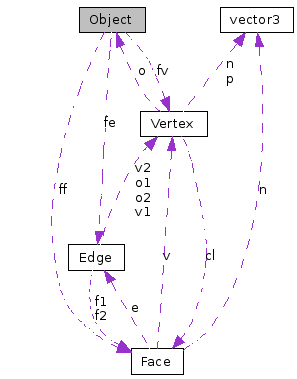
\includegraphics[width=129pt]{classObject__coll__graph}
\end{center}
\end{figure}
\subsection*{Public Member Functions}
\begin{CompactItemize}
\item 
{\bf Object} (std::string)
\item 
{\bf Object} ({\bf Object} const \&)
\item 
{\bf Object} \& {\bf operator=} ({\bf Object} const \&)
\item 
void {\bf find\-Vert\-Adj} (void)
\item 
void {\bf bound\-Object} (double $\ast$const \&) const
\item 
void {\bf set\-FF} ({\bf Face} $\ast$)
\item 
void {\bf set\-FV} ({\bf Vertex} $\ast$)
\item 
{\bf Edge} $\ast$ {\bf get\-FE} (void) const
\item 
{\bf Face} $\ast$ {\bf get\-FF} (void) const
\item 
{\bf Vertex} $\ast$ {\bf get\-FV} (void) const
\item 
std::string const \& {\bf get\-Name} (void) const
\item 
int {\bf set\-Num\-Digits} (void) const
\item 
void {\bf create\-Edges} (void)
\item 
void {\bf process\-Edge} ({\bf Face} $\ast$const, {\bf Vertex} $\ast$const, {\bf Vertex} $\ast$const, {\bf Vertex} $\ast$const, {\bf map\_\-s\_\-ep} \&, int const \&)
\item 
void {\bf create\-Edge} ({\bf Face} $\ast$const, {\bf Vertex} $\ast$const, {\bf Vertex} $\ast$const, {\bf Vertex} $\ast$const, {\bf map\_\-s\_\-ep} \&, int const \&)
\item 
{\bf Edge} $\ast$ {\bf find\-Edge} ({\bf Vertex} const $\ast$const, {\bf Vertex} const $\ast$const, {\bf map\_\-s\_\-ep} const \&, int const \&) const
\item 
std::string {\bf key\-Pair} (int const \&a, int const \&b, int const \&num\_\-digits) const
\end{CompactItemize}
\subsection*{Public Attributes}
\begin{CompactItemize}
\item 
{\bf vec\_\-v} {\bf v}
\item 
{\bf vec\_\-f} {\bf f}
\item 
{\bf vec\_\-e} {\bf e}
\end{CompactItemize}


\subsection{Constructor \& Destructor Documentation}
\index{Object@{Object}!Object@{Object}}
\index{Object@{Object}!Object@{Object}}
\subsubsection{\setlength{\rightskip}{0pt plus 5cm}Object::Object (std::string)}\label{classObject_9726153b1164522a3244fcb885870a99}


\index{Object@{Object}!Object@{Object}}
\index{Object@{Object}!Object@{Object}}
\subsubsection{\setlength{\rightskip}{0pt plus 5cm}Object::Object ({\bf Object} const \&)}\label{classObject_6e166f85639b15a8b8f9b783a6de3b45}




\subsection{Member Function Documentation}
\index{Object@{Object}!operator=@{operator=}}
\index{operator=@{operator=}!Object@{Object}}
\subsubsection{\setlength{\rightskip}{0pt plus 5cm}{\bf Object} \& Object::operator= ({\bf Object} const \&)}\label{classObject_d5a622757f2d91f0b3fc41b8af751d6f}


\index{Object@{Object}!findVertAdj@{findVertAdj}}
\index{findVertAdj@{findVertAdj}!Object@{Object}}
\subsubsection{\setlength{\rightskip}{0pt plus 5cm}void Object::find\-Vert\-Adj (void)}\label{classObject_2489fb94c4141ad5cd692fdb9d9019e9}


Record in vertex class adjacent faces to each vertex in this object. \index{Object@{Object}!boundObject@{boundObject}}
\index{boundObject@{boundObject}!Object@{Object}}
\subsubsection{\setlength{\rightskip}{0pt plus 5cm}void Object::bound\-Object (double $\ast$const \& {\em bounding\_\-box}) const}\label{classObject_40b6fe0262440f577e2c661dc118e9dc}


Compute and return bounding box of this object along principal directions. \begin{Desc}
\item[Parameters:]
\begin{description}
\item[\mbox{$\rightarrow$} {\em bounding\_\-box}]Bounding box of object as (xmin,xmax,ymin,ymax,zmin,zmax). \end{description}
\end{Desc}
\index{Object@{Object}!setFF@{setFF}}
\index{setFF@{setFF}!Object@{Object}}
\subsubsection{\setlength{\rightskip}{0pt plus 5cm}void Object::set\-FF ({\bf Face} $\ast$ {\em fptr})}\label{classObject_b6f62e2bd7a446660a1c4edddbc54c43}


Record pointer to first face in face vector. \begin{Desc}
\item[Parameters:]
\begin{description}
\item[\mbox{$\leftarrow$} {\em fptr}]Pointer to first face. \end{description}
\end{Desc}
\index{Object@{Object}!setFV@{setFV}}
\index{setFV@{setFV}!Object@{Object}}
\subsubsection{\setlength{\rightskip}{0pt plus 5cm}void Object::set\-FV ({\bf Vertex} $\ast$ {\em vv})}\label{classObject_f0c78579e86899e317de5c13ca376578}


Record pointer to first vertex in vertex vector. \begin{Desc}
\item[Parameters:]
\begin{description}
\item[\mbox{$\leftarrow$} {\em vv}]Pointer to first vertex. \end{description}
\end{Desc}
\index{Object@{Object}!getFE@{getFE}}
\index{getFE@{getFE}!Object@{Object}}
\subsubsection{\setlength{\rightskip}{0pt plus 5cm}{\bf Edge} $\ast$ Object::get\-FE (void) const}\label{classObject_f29ab111dc99b3bd5f3aa2909d95cbcb}


Return pointer to recorded first edge in edge vector. \begin{Desc}
\item[Returns:]Pointer to first edge. \end{Desc}
\index{Object@{Object}!getFF@{getFF}}
\index{getFF@{getFF}!Object@{Object}}
\subsubsection{\setlength{\rightskip}{0pt plus 5cm}{\bf Face} $\ast$ Object::get\-FF (void) const}\label{classObject_cf73cd78612c003fcd8898c3a6aadf3a}


Return pointer to recorded first face in face vector. \begin{Desc}
\item[Returns:]Pointer to first face. \end{Desc}
\index{Object@{Object}!getFV@{getFV}}
\index{getFV@{getFV}!Object@{Object}}
\subsubsection{\setlength{\rightskip}{0pt plus 5cm}{\bf Vertex} $\ast$ Object::get\-FV (void) const}\label{classObject_01ba19ef93138092e00449c5a2afe662}


Return pointer to recorded first vertex in vertex vector. \begin{Desc}
\item[Returns:]Pointer to first vertex. \end{Desc}
\index{Object@{Object}!getName@{getName}}
\index{getName@{getName}!Object@{Object}}
\subsubsection{\setlength{\rightskip}{0pt plus 5cm}std::string const \& Object::get\-Name (void) const}\label{classObject_13c8bbe670573a1af1c3c316a57b92a0}


Get recorded name of this object. \begin{Desc}
\item[Returns:]\doxyref{Object}{p.}{classObject} name. \end{Desc}
\index{Object@{Object}!setNumDigits@{setNumDigits}}
\index{setNumDigits@{setNumDigits}!Object@{Object}}
\subsubsection{\setlength{\rightskip}{0pt plus 5cm}int Object::set\-Num\-Digits (void) const}\label{classObject_380cd57bfc576a026727e9b110c13c3c}


Determine the length in digits of largest vertex index. \begin{Desc}
\item[Returns:]Number of digits required for larget vertex index. \end{Desc}
\index{Object@{Object}!createEdges@{createEdges}}
\index{createEdges@{createEdges}!Object@{Object}}
\subsubsection{\setlength{\rightskip}{0pt plus 5cm}void Object::create\-Edges (void)}\label{classObject_f7b4257697cf8cb9bdc289b80596e996}


\index{Object@{Object}!processEdge@{processEdge}}
\index{processEdge@{processEdge}!Object@{Object}}
\subsubsection{\setlength{\rightskip}{0pt plus 5cm}void Object::process\-Edge ({\bf Face} $\ast$ const {\em face}, {\bf Vertex} $\ast$ const {\em va}, {\bf Vertex} $\ast$ const {\em vb}, {\bf Vertex} $\ast$ const {\em vc}, {\bf map\_\-s\_\-ep} \& {\em hm}, int const \& {\em num\_\-digits})}\label{classObject_92a3557cc1df954d7bf78418f79f1a45}


Record input face edge information as \doxyref{Edge}{p.}{classEdge} class instance. \begin{Desc}
\item[Parameters:]
\begin{description}
\item[\mbox{$\leftarrow$} {\em face}]Parent face. \item[\mbox{$\leftarrow$} {\em va}]One vertex of edge from parent face. \item[\mbox{$\leftarrow$} {\em vb}]Other vertex of edge from parent face. \item[\mbox{$\leftarrow$} {\em vc}]\doxyref{Vertex}{p.}{classVertex} from parent face not on edge. \item[\mbox{$\leftarrow$} {\em hm}]Map for finding existing edges with vertex indices as key. \item[\mbox{$\leftarrow$} {\em num\_\-digits}]Number of digits used in maximum integer value. \end{description}
\end{Desc}
\index{Object@{Object}!createEdge@{createEdge}}
\index{createEdge@{createEdge}!Object@{Object}}
\subsubsection{\setlength{\rightskip}{0pt plus 5cm}void Object::create\-Edge ({\bf Face} $\ast$ const {\em face}, {\bf Vertex} $\ast$ const {\em va}, {\bf Vertex} $\ast$ const {\em vb}, {\bf Vertex} $\ast$ const {\em vc}, {\bf map\_\-s\_\-ep} \& {\em hm}, int const \& {\em num\_\-digits})}\label{classObject_4ba1e14d7e3a89f93808bd17b13c63ba}


Create and record new instance of \doxyref{Edge}{p.}{classEdge} class. \begin{Desc}
\item[Parameters:]
\begin{description}
\item[\mbox{$\leftarrow$} {\em face}]Parent face. \item[\mbox{$\leftarrow$} {\em va}]One vertex of edge from parent face. \item[\mbox{$\leftarrow$} {\em vb}]Other vertex of edge from parent face. \item[\mbox{$\leftarrow$} {\em vc}]\doxyref{Vertex}{p.}{classVertex} from parent face not on edge. \item[\mbox{$\leftarrow$} {\em hm}]Map for finding existing edges with vertex indices as key. \item[\mbox{$\leftarrow$} {\em num\_\-digits}]Number of digits used in maximum integer value. \end{description}
\end{Desc}
\index{Object@{Object}!findEdge@{findEdge}}
\index{findEdge@{findEdge}!Object@{Object}}
\subsubsection{\setlength{\rightskip}{0pt plus 5cm}{\bf Edge} $\ast$ Object::find\-Edge ({\bf Vertex} const $\ast$ const {\em va}, {\bf Vertex} const $\ast$ const {\em vb}, {\bf map\_\-s\_\-ep} const \& {\em hm}, int const \& {\em num\_\-digits}) const}\label{classObject_5bf479c6d31a29b8c9cf9a20eb0b923c}


Look for matching recorded edge instance. \begin{Desc}
\item[Parameters:]
\begin{description}
\item[\mbox{$\leftarrow$} {\em va}]One vertex of edge from parent face. \item[\mbox{$\leftarrow$} {\em vb}]Other vertex of edge from parent face. \item[\mbox{$\leftarrow$} {\em hm}]Map for finding existing edges with vertex indices as key. \item[\mbox{$\leftarrow$} {\em num\_\-digits}]Number of digits used in maximum integer value. \end{description}
\end{Desc}
\begin{Desc}
\item[Returns:]\doxyref{Edge}{p.}{classEdge} pointer if match found; NULL otherwise; \end{Desc}
\index{Object@{Object}!keyPair@{keyPair}}
\index{keyPair@{keyPair}!Object@{Object}}
\subsubsection{\setlength{\rightskip}{0pt plus 5cm}std::string Object::key\-Pair (int const \& {\em a}, int const \& {\em b}, int const \& {\em num\_\-digits}) const}\label{classObject_3babf3bd25fd46dfd69898c544c7babd}


Create a unique string from two input integers. \begin{Desc}
\item[Parameters:]
\begin{description}
\item[\mbox{$\leftarrow$} {\em a}]First integer. \item[\mbox{$\leftarrow$} {\em b}]Second integer. \item[\mbox{$\leftarrow$} {\em num\_\-digits}]Number of digits used in maximum integer value. \end{description}
\end{Desc}
\begin{Desc}
\item[Returns:]Unique string including two input integers. \end{Desc}


\subsection{Member Data Documentation}
\index{Object@{Object}!v@{v}}
\index{v@{v}!Object@{Object}}
\subsubsection{\setlength{\rightskip}{0pt plus 5cm}{\bf vec\_\-v} {\bf Object::v}}\label{classObject_f50cb9c150ab8493111dcf29170b23fc}


\index{Object@{Object}!f@{f}}
\index{f@{f}!Object@{Object}}
\subsubsection{\setlength{\rightskip}{0pt plus 5cm}{\bf vec\_\-f} {\bf Object::f}}\label{classObject_ec66102e74e431c089c6ce171e365002}


\index{Object@{Object}!e@{e}}
\index{e@{e}!Object@{Object}}
\subsubsection{\setlength{\rightskip}{0pt plus 5cm}{\bf vec\_\-e} {\bf Object::e}}\label{classObject_8906949fbfe42985f4cd33154abe2835}




The documentation for this class was generated from the following files:\begin{CompactItemize}
\item 
{\bf object.h}\item 
{\bf object.cc}\end{CompactItemize}

\hypertarget{classParameter}{
\section{Parameter Class Reference}
\label{classParameter}\index{Parameter@{Parameter}}
}
{\tt \#include $<$parameter.h$>$}

\subsection*{Public Member Functions}
\begin{CompactItemize}
\item 
void \hyperlink{classParameter_54d870873dcf44d515ab5384a38de7af}{print} (char const $\ast$const filename) const 
\item 
void \hyperlink{classParameter_c3fd9360e62e3b9fe764a95e8f3e2b50}{computeDeviations} (const std::vector$<$ \hyperlink{classPoint}{Point} $>$ \&raw\_\-points)
\item 
void \hyperlink{classParameter_918287332cac92ccf75c78fb651efc97}{getRawPointsToDuplicate} (const std::vector$<$ \hyperlink{classPoint}{Point} $>$ \&raw\_\-points, std::vector$<$ int $>$ \&raw\_\-points\_\-to\_\-duplicate) const 
\item 
double \hyperlink{classParameter_db51977acf04748c2d4a82a619459c0d}{calcMinDistPtLineSegment} (const \hyperlink{classPoint}{Point} \&spline\_\-sample, const \hyperlink{classPoint}{Point} \&contour\_\-point\_\-1, const \hyperlink{classPoint}{Point} \&contour\_\-point\_\-3) const 
\item 
void \hyperlink{classParameter_ff6c2b408f89720293ec4db6ef186c3f}{addDeviation} (double d)
\item 
\hyperlink{classParameter_b1939f6d4bacbd505ead9dfafcd2647f}{Parameter} (void)
\item 
bool \hyperlink{classParameter_ec98b30f1dfebcb04e504adadb4a5787}{deviationsLarge} (void)
\item 
void \hyperlink{classParameter_8db6db4bd306208ccfbf94ef04d39955}{reserve} (const int \&target\_\-num\_\-samples)
\item 
\hyperlink{classPoint}{Point} const $\ast$ \hyperlink{classParameter_21bfc1fa9f7999cd18429493fef88485}{getPoint} (const int \&sample\_\-index) const 
\item 
void \hyperlink{classParameter_90c14f9388c291ebd0199b542ea3eaa2}{clearAndReserveSamples} (void)
\item 
void \hyperlink{classParameter_baa819bda68eaca98d6d78bde5c65f1b}{add} (const double \&path\_\-parameter\_\-value, const int \&index\_\-of\_\-spline, const double \&delta\_\-s\_\-to\_\-lhs)
\item 
void \hyperlink{classParameter_d0a92d44cf3746bfae006c5761b862d1}{set} (double new\_\-s, int new\_\-spline\_\-index, int sample\_\-index, double s\_\-disp, \hyperlink{classPoint}{Point} p)
\item 
int \hyperlink{classParameter_e6a494adb7a970b6d9a1d6c242f600e6}{getNumSamplePoints} (void) const 
\item 
int \hyperlink{classParameter_51f0d8dc2f9c7c113be49351118902e2}{getNumSamples} (void) const 
\item 
double \hyperlink{classParameter_2f0b21ed83fb3a11305ee733a34317b2}{getParameterValue} (int sample\_\-index) const 
\item 
int \hyperlink{classParameter_3f630390b0346479113e758df49ad21d}{getSplineIndex} (int sample\_\-index) const 
\item 
double \hyperlink{classParameter_b918e85afbde855a65c0b82cb3484308}{getLhsS} (int sample\_\-index) const 
\item 
void \hyperlink{classParameter_52053a1e39332eab88503c5328343d7f}{addSplineSample} (\hyperlink{classPoint}{Point} p)
\item 
\hyperlink{parameter_8h_76617663fb8c2b14cf698a47a4d07926}{c\_\-d\_\-iterator} \hyperlink{classParameter_69d4f2f72a57ac999196a1b7d3417286}{getFirstDeviationConst} (void) const 
\item 
\hyperlink{parameter_8h_76617663fb8c2b14cf698a47a4d07926}{c\_\-d\_\-iterator} \hyperlink{classParameter_fc243c9ebaef7c8711859696d8c5a1a4}{getOnePastLastDeviationConst} (void) const 
\item 
\hyperlink{parameter_8h_d367c52cb5a031e4bc21ba9af7d6ee47}{c\_\-p\_\-iterator} \hyperlink{classParameter_7006d1d623467ddf4c94724503ee77d5}{getFirstSplineSampleConst} (void) const 
\item 
\hyperlink{parameter_8h_d367c52cb5a031e4bc21ba9af7d6ee47}{c\_\-p\_\-iterator} \hyperlink{classParameter_bab72e16fa4732267560e6b0b661fb8b}{getOnePastLastSplineSampleConst} (void) const 
\end{CompactItemize}


\subsection{Constructor \& Destructor Documentation}
\hypertarget{classParameter_b1939f6d4bacbd505ead9dfafcd2647f}{
\index{Parameter@{Parameter}!Parameter@{Parameter}}
\index{Parameter@{Parameter}!Parameter@{Parameter}}
\subsubsection[Parameter]{\setlength{\rightskip}{0pt plus 5cm}Parameter::Parameter (void)\hspace{0.3cm}{\tt  \mbox{[}inline\mbox{]}}}}
\label{classParameter_b1939f6d4bacbd505ead9dfafcd2647f}




\subsection{Member Function Documentation}
\hypertarget{classParameter_54d870873dcf44d515ab5384a38de7af}{
\index{Parameter@{Parameter}!print@{print}}
\index{print@{print}!Parameter@{Parameter}}
\subsubsection[print]{\setlength{\rightskip}{0pt plus 5cm}void Parameter::print (char const $\ast$const  {\em filename}) const}}
\label{classParameter_54d870873dcf44d515ab5384a38de7af}


Write path parameter values, spline indices, and path parameter distances to left-hand side sample point to file. \begin{Desc}
\item[Parameters:]
\begin{description}
\item[\mbox{$\leftarrow$} {\em filename}]Output file name. \end{description}
\end{Desc}


Referenced by Contour::processContour(), and Contour::writeFilesAfter().\hypertarget{classParameter_c3fd9360e62e3b9fe764a95e8f3e2b50}{
\index{Parameter@{Parameter}!computeDeviations@{computeDeviations}}
\index{computeDeviations@{computeDeviations}!Parameter@{Parameter}}
\subsubsection[computeDeviations]{\setlength{\rightskip}{0pt plus 5cm}void Parameter::computeDeviations (const std::vector$<$ {\bf Point} $>$ \& {\em raw\_\-points})}}
\label{classParameter_c3fd9360e62e3b9fe764a95e8f3e2b50}


Calculate perpendicular distance between each spline samples and nearest linearly-interpolated raw contour points. \begin{Desc}
\item[Parameters:]
\begin{description}
\item[\mbox{$\leftarrow$} {\em raw\_\-points}]All original points in contour. \end{description}
\end{Desc}


References calcMinDistPtLineSegment().

Referenced by Contour::computeDeviations().\hypertarget{classParameter_918287332cac92ccf75c78fb651efc97}{
\index{Parameter@{Parameter}!getRawPointsToDuplicate@{getRawPointsToDuplicate}}
\index{getRawPointsToDuplicate@{getRawPointsToDuplicate}!Parameter@{Parameter}}
\subsubsection[getRawPointsToDuplicate]{\setlength{\rightskip}{0pt plus 5cm}void Parameter::getRawPointsToDuplicate (const std::vector$<$ {\bf Point} $>$ \& {\em raw\_\-points}, \/  std::vector$<$ int $>$ \& {\em raw\_\-points\_\-to\_\-duplicate}) const}}
\label{classParameter_918287332cac92ccf75c78fb651efc97}


Determine which control points of splines to duplicate to reduce deviation between spline samples and linearly-interpolated raw contour points. \begin{Desc}
\item[Parameters:]
\begin{description}
\item[\mbox{$\leftarrow$} {\em raw\_\-points}]All original points in contour. \item[\mbox{$\rightarrow$} {\em raw\_\-points\_\-to\_\-duplicate}]Raw points that should be duplicated as control points. \end{description}
\end{Desc}


References Controls::getDeviationThreshold(), and Controls::instance().

Referenced by Contour::duplicateControlPoints().\hypertarget{classParameter_db51977acf04748c2d4a82a619459c0d}{
\index{Parameter@{Parameter}!calcMinDistPtLineSegment@{calcMinDistPtLineSegment}}
\index{calcMinDistPtLineSegment@{calcMinDistPtLineSegment}!Parameter@{Parameter}}
\subsubsection[calcMinDistPtLineSegment]{\setlength{\rightskip}{0pt plus 5cm}double Parameter::calcMinDistPtLineSegment (const {\bf Point} \& {\em spline\_\-sample}, \/  const {\bf Point} \& {\em contour\_\-point\_\-1}, \/  const {\bf Point} \& {\em contour\_\-point\_\-2}) const}}
\label{classParameter_db51977acf04748c2d4a82a619459c0d}


Calculate perpendicular distance from sample point to nearest raw contour point line segment. \begin{Desc}
\item[Parameters:]
\begin{description}
\item[\mbox{$\leftarrow$} {\em spline\_\-sample}]Spline sample point of interest. \item[\mbox{$\leftarrow$} {\em contour\_\-point\_\-1}]One end of line segment. \item[\mbox{$\leftarrow$} {\em contour\_\-point\_\-2}]Other end of line segment. \end{description}
\end{Desc}
\begin{Desc}
\item[Returns:]Perpendicular distance from sample\_\-point to line segment. \end{Desc}


References Point::dot(), and Point::length().

Referenced by computeDeviations().\hypertarget{classParameter_ff6c2b408f89720293ec4db6ef186c3f}{
\index{Parameter@{Parameter}!addDeviation@{addDeviation}}
\index{addDeviation@{addDeviation}!Parameter@{Parameter}}
\subsubsection[addDeviation]{\setlength{\rightskip}{0pt plus 5cm}void Parameter::addDeviation (double {\em d})\hspace{0.3cm}{\tt  \mbox{[}inline\mbox{]}}}}
\label{classParameter_ff6c2b408f89720293ec4db6ef186c3f}




Referenced by Contour::setSamplesToRaw().\hypertarget{classParameter_ec98b30f1dfebcb04e504adadb4a5787}{
\index{Parameter@{Parameter}!deviationsLarge@{deviationsLarge}}
\index{deviationsLarge@{deviationsLarge}!Parameter@{Parameter}}
\subsubsection[deviationsLarge]{\setlength{\rightskip}{0pt plus 5cm}bool Parameter::deviationsLarge (void)\hspace{0.3cm}{\tt  \mbox{[}inline\mbox{]}}}}
\label{classParameter_ec98b30f1dfebcb04e504adadb4a5787}


Determine if any deviation of sample points exceeds threshold. 

References Controls::getDeviationThreshold(), and Controls::instance().

Referenced by Contour::deviationsLarge().\hypertarget{classParameter_8db6db4bd306208ccfbf94ef04d39955}{
\index{Parameter@{Parameter}!reserve@{reserve}}
\index{reserve@{reserve}!Parameter@{Parameter}}
\subsubsection[reserve]{\setlength{\rightskip}{0pt plus 5cm}void Parameter::reserve (const int \& {\em target\_\-num\_\-samples})\hspace{0.3cm}{\tt  \mbox{[}inline\mbox{]}}}}
\label{classParameter_8db6db4bd306208ccfbf94ef04d39955}


Clear all class data and allocate memory. \begin{Desc}
\item[Parameters:]
\begin{description}
\item[\mbox{$\leftarrow$} {\em target\_\-num\_\-samples}]Amount of memory to reserve for future data. \end{description}
\end{Desc}


Referenced by Contour::processContour().\hypertarget{classParameter_21bfc1fa9f7999cd18429493fef88485}{
\index{Parameter@{Parameter}!getPoint@{getPoint}}
\index{getPoint@{getPoint}!Parameter@{Parameter}}
\subsubsection[getPoint]{\setlength{\rightskip}{0pt plus 5cm}{\bf Point} const$\ast$ Parameter::getPoint (const int \& {\em sample\_\-index}) const\hspace{0.3cm}{\tt  \mbox{[}inline\mbox{]}}}}
\label{classParameter_21bfc1fa9f7999cd18429493fef88485}


Get sample point. \begin{Desc}
\item[Parameters:]
\begin{description}
\item[\mbox{$\leftarrow$} {\em sample\_\-index}]Index of sample point of interest. \end{description}
\end{Desc}
\begin{Desc}
\item[Returns:]Sample point. \end{Desc}
\hypertarget{classParameter_90c14f9388c291ebd0199b542ea3eaa2}{
\index{Parameter@{Parameter}!clearAndReserveSamples@{clearAndReserveSamples}}
\index{clearAndReserveSamples@{clearAndReserveSamples}!Parameter@{Parameter}}
\subsubsection[clearAndReserveSamples]{\setlength{\rightskip}{0pt plus 5cm}void Parameter::clearAndReserveSamples (void)\hspace{0.3cm}{\tt  \mbox{[}inline\mbox{]}}}}
\label{classParameter_90c14f9388c291ebd0199b542ea3eaa2}


Clear samples and reallocate memory. \hypertarget{classParameter_baa819bda68eaca98d6d78bde5c65f1b}{
\index{Parameter@{Parameter}!add@{add}}
\index{add@{add}!Parameter@{Parameter}}
\subsubsection[add]{\setlength{\rightskip}{0pt plus 5cm}void Parameter::add (const double \& {\em path\_\-parameter\_\-value}, \/  const int \& {\em index\_\-of\_\-spline}, \/  const double \& {\em delta\_\-s\_\-to\_\-lhs})\hspace{0.3cm}{\tt  \mbox{[}inline\mbox{]}}}}
\label{classParameter_baa819bda68eaca98d6d78bde5c65f1b}


Add sample point. \begin{Desc}
\item[Parameters:]
\begin{description}
\item[\mbox{$\leftarrow$} {\em path\_\-parameter\_\-value}]Path parameter value of sample point for spline. \item[\mbox{$\leftarrow$} {\em index\_\-of\_\-spline}]Index of spline on which sample point lies. \item[\mbox{$\leftarrow$} {\em delta\_\-s\_\-to\_\-lhs}]Path parameter distance to nearest sample point to the left. \end{description}
\end{Desc}
\hypertarget{classParameter_d0a92d44cf3746bfae006c5761b862d1}{
\index{Parameter@{Parameter}!set@{set}}
\index{set@{set}!Parameter@{Parameter}}
\subsubsection[set]{\setlength{\rightskip}{0pt plus 5cm}void Parameter::set (double {\em new\_\-s}, \/  int {\em new\_\-spline\_\-index}, \/  int {\em sample\_\-index}, \/  double {\em s\_\-disp}, \/  {\bf Point} {\em p})\hspace{0.3cm}{\tt  \mbox{[}inline\mbox{]}}}}
\label{classParameter_d0a92d44cf3746bfae006c5761b862d1}


Move spline sample point. \begin{Desc}
\item[Parameters:]
\begin{description}
\item[\mbox{$\leftarrow$} {\em new\_\-s}]New path parameter value. \item[\mbox{$\leftarrow$} {\em new\_\-spline\_\-index}]Index of new spline on which point sits. \item[\mbox{$\leftarrow$} {\em sample\_\-index}]Index of sample point being moved. \item[\mbox{$\leftarrow$} {\em s\_\-disp}]Change in path parameter value from old value. Signed value. \item[\mbox{$\leftarrow$} {\em p}]New location of sample point. \end{description}
\end{Desc}


References getNumSamples().\hypertarget{classParameter_e6a494adb7a970b6d9a1d6c242f600e6}{
\index{Parameter@{Parameter}!getNumSamplePoints@{getNumSamplePoints}}
\index{getNumSamplePoints@{getNumSamplePoints}!Parameter@{Parameter}}
\subsubsection[getNumSamplePoints]{\setlength{\rightskip}{0pt plus 5cm}int Parameter::getNumSamplePoints (void) const\hspace{0.3cm}{\tt  \mbox{[}inline\mbox{]}}}}
\label{classParameter_e6a494adb7a970b6d9a1d6c242f600e6}




Referenced by Contour::getNumSamplePoints(), Contour::isDegenerate(), and Contour::printPtsFiles().\hypertarget{classParameter_51f0d8dc2f9c7c113be49351118902e2}{
\index{Parameter@{Parameter}!getNumSamples@{getNumSamples}}
\index{getNumSamples@{getNumSamples}!Parameter@{Parameter}}
\subsubsection[getNumSamples]{\setlength{\rightskip}{0pt plus 5cm}int Parameter::getNumSamples (void) const\hspace{0.3cm}{\tt  \mbox{[}inline\mbox{]}}}}
\label{classParameter_51f0d8dc2f9c7c113be49351118902e2}




Referenced by Contour::printSplineSamplesHere(), and set().\hypertarget{classParameter_2f0b21ed83fb3a11305ee733a34317b2}{
\index{Parameter@{Parameter}!getParameterValue@{getParameterValue}}
\index{getParameterValue@{getParameterValue}!Parameter@{Parameter}}
\subsubsection[getParameterValue]{\setlength{\rightskip}{0pt plus 5cm}double Parameter::getParameterValue (int {\em sample\_\-index}) const\hspace{0.3cm}{\tt  \mbox{[}inline\mbox{]}}}}
\label{classParameter_2f0b21ed83fb3a11305ee733a34317b2}


\hypertarget{classParameter_3f630390b0346479113e758df49ad21d}{
\index{Parameter@{Parameter}!getSplineIndex@{getSplineIndex}}
\index{getSplineIndex@{getSplineIndex}!Parameter@{Parameter}}
\subsubsection[getSplineIndex]{\setlength{\rightskip}{0pt plus 5cm}int Parameter::getSplineIndex (int {\em sample\_\-index}) const\hspace{0.3cm}{\tt  \mbox{[}inline\mbox{]}}}}
\label{classParameter_3f630390b0346479113e758df49ad21d}


\hypertarget{classParameter_b918e85afbde855a65c0b82cb3484308}{
\index{Parameter@{Parameter}!getLhsS@{getLhsS}}
\index{getLhsS@{getLhsS}!Parameter@{Parameter}}
\subsubsection[getLhsS]{\setlength{\rightskip}{0pt plus 5cm}double Parameter::getLhsS (int {\em sample\_\-index}) const\hspace{0.3cm}{\tt  \mbox{[}inline\mbox{]}}}}
\label{classParameter_b918e85afbde855a65c0b82cb3484308}


\hypertarget{classParameter_52053a1e39332eab88503c5328343d7f}{
\index{Parameter@{Parameter}!addSplineSample@{addSplineSample}}
\index{addSplineSample@{addSplineSample}!Parameter@{Parameter}}
\subsubsection[addSplineSample]{\setlength{\rightskip}{0pt plus 5cm}void Parameter::addSplineSample ({\bf Point} {\em p})\hspace{0.3cm}{\tt  \mbox{[}inline\mbox{]}}}}
\label{classParameter_52053a1e39332eab88503c5328343d7f}




Referenced by Contour::setSamplesToRaw().\hypertarget{classParameter_69d4f2f72a57ac999196a1b7d3417286}{
\index{Parameter@{Parameter}!getFirstDeviationConst@{getFirstDeviationConst}}
\index{getFirstDeviationConst@{getFirstDeviationConst}!Parameter@{Parameter}}
\subsubsection[getFirstDeviationConst]{\setlength{\rightskip}{0pt plus 5cm}{\bf c\_\-d\_\-iterator} Parameter::getFirstDeviationConst (void) const\hspace{0.3cm}{\tt  \mbox{[}inline\mbox{]}}}}
\label{classParameter_69d4f2f72a57ac999196a1b7d3417286}




Referenced by Contour::firstDeviation(), and Contour::updateDeviations().\hypertarget{classParameter_fc243c9ebaef7c8711859696d8c5a1a4}{
\index{Parameter@{Parameter}!getOnePastLastDeviationConst@{getOnePastLastDeviationConst}}
\index{getOnePastLastDeviationConst@{getOnePastLastDeviationConst}!Parameter@{Parameter}}
\subsubsection[getOnePastLastDeviationConst]{\setlength{\rightskip}{0pt plus 5cm}{\bf c\_\-d\_\-iterator} Parameter::getOnePastLastDeviationConst (void) const\hspace{0.3cm}{\tt  \mbox{[}inline\mbox{]}}}}
\label{classParameter_fc243c9ebaef7c8711859696d8c5a1a4}




Referenced by Contour::onePastLastDeviation(), and Contour::updateDeviations().\hypertarget{classParameter_7006d1d623467ddf4c94724503ee77d5}{
\index{Parameter@{Parameter}!getFirstSplineSampleConst@{getFirstSplineSampleConst}}
\index{getFirstSplineSampleConst@{getFirstSplineSampleConst}!Parameter@{Parameter}}
\subsubsection[getFirstSplineSampleConst]{\setlength{\rightskip}{0pt plus 5cm}{\bf c\_\-p\_\-iterator} Parameter::getFirstSplineSampleConst (void) const\hspace{0.3cm}{\tt  \mbox{[}inline\mbox{]}}}}
\label{classParameter_7006d1d623467ddf4c94724503ee77d5}




Referenced by Contour::calcSampleIntervals(), Contour::printPtsFiles(), and Contour::updateSampleIntervals().\hypertarget{classParameter_bab72e16fa4732267560e6b0b661fb8b}{
\index{Parameter@{Parameter}!getOnePastLastSplineSampleConst@{getOnePastLastSplineSampleConst}}
\index{getOnePastLastSplineSampleConst@{getOnePastLastSplineSampleConst}!Parameter@{Parameter}}
\subsubsection[getOnePastLastSplineSampleConst]{\setlength{\rightskip}{0pt plus 5cm}{\bf c\_\-p\_\-iterator} Parameter::getOnePastLastSplineSampleConst (void) const\hspace{0.3cm}{\tt  \mbox{[}inline\mbox{]}}}}
\label{classParameter_bab72e16fa4732267560e6b0b661fb8b}




Referenced by Contour::calcSampleIntervals(), Contour::printPtsFiles(), and Contour::updateSampleIntervals().

The documentation for this class was generated from the following files:\begin{CompactItemize}
\item 
\hyperlink{parameter_8h}{parameter.h}\item 
\hyperlink{parameter_8cc}{parameter.cc}\end{CompactItemize}

\hypertarget{classPoint}{
\section{Point Class Reference}
\label{classPoint}\index{Point@{Point}}
}
{\tt \#include $<$point.h$>$}

\subsection*{Public Member Functions}
\begin{CompactItemize}
\item 
\hyperlink{classPoint_94dc19d9beda0018169bd5ef8cd730c3}{Point} (void)
\item 
\hyperlink{classPoint_2a6d8ce5866c8d0e4e5c9d659ce6bfc2}{Point} (char const $\ast$str, double $\ast$const transform)
\item 
\hyperlink{classPoint_25ceb467297fed76765cde5c9ff20fa4}{Point} (double xval, double yval)
\item 
double \hyperlink{classPoint_b73ba91268c3d3b783fd2a0983066b38}{getX} (void) const 
\item 
double \hyperlink{classPoint_1b00b67b5e96ce7e02011c170f07bf11}{getY} (void) const 
\item 
void \hyperlink{classPoint_9290a4098a3331e34f158eeca694a26c}{setX} (double i)
\item 
void \hyperlink{classPoint_387c7e206f5ba0ea575020e53a66fb55}{setY} (double i)
\item 
void \hyperlink{classPoint_67517850a2ef6cfe8d6beb161be65e5c}{print} (char $\ast$const line) const 
\item 
\hyperlink{classPoint}{Point} \hyperlink{classPoint_6a869eababaaf863740e3196b9ca6780}{operator-} (const \hyperlink{classPoint}{Point} \&p) const 
\item 
double \hyperlink{classPoint_a51050f8b9868c12b1a9d063e8555d05}{dot} (const \hyperlink{classPoint}{Point} \&p) const 
\item 
double \hyperlink{classPoint_99717644bf38e3868c9ff7f32f4a9226}{distance\_\-squared} (const \hyperlink{classPoint}{Point} \&p) const 
\item 
double \hyperlink{classPoint_41052067de2f7e0be2bf0b60c1e7f60d}{length} (void) const 
\item 
\hyperlink{classPoint}{Point} \& \hyperlink{classPoint_aed1420449367308540f3459049ac2bd}{operator$\ast$=} (double \hyperlink{proximity__energy_8m_4124bc0a9335c27f086f24ba207a4912}{a})
\end{CompactItemize}


\subsection{Constructor \& Destructor Documentation}
\hypertarget{classPoint_94dc19d9beda0018169bd5ef8cd730c3}{
\index{Point@{Point}!Point@{Point}}
\index{Point@{Point}!Point@{Point}}
\subsubsection[Point]{\setlength{\rightskip}{0pt plus 5cm}Point::Point (void)}}
\label{classPoint_94dc19d9beda0018169bd5ef8cd730c3}




Referenced by operator-().\hypertarget{classPoint_2a6d8ce5866c8d0e4e5c9d659ce6bfc2}{
\index{Point@{Point}!Point@{Point}}
\index{Point@{Point}!Point@{Point}}
\subsubsection[Point]{\setlength{\rightskip}{0pt plus 5cm}Point::Point (char const $\ast$ {\em str}, \/  double $\ast$const  {\em transform})}}
\label{classPoint_2a6d8ce5866c8d0e4e5c9d659ce6bfc2}


\hypertarget{classPoint_25ceb467297fed76765cde5c9ff20fa4}{
\index{Point@{Point}!Point@{Point}}
\index{Point@{Point}!Point@{Point}}
\subsubsection[Point]{\setlength{\rightskip}{0pt plus 5cm}Point::Point (double {\em xval}, \/  double {\em yval})}}
\label{classPoint_25ceb467297fed76765cde5c9ff20fa4}




\subsection{Member Function Documentation}
\hypertarget{classPoint_b73ba91268c3d3b783fd2a0983066b38}{
\index{Point@{Point}!getX@{getX}}
\index{getX@{getX}!Point@{Point}}
\subsubsection[getX]{\setlength{\rightskip}{0pt plus 5cm}double Point::getX (void) const\hspace{0.3cm}{\tt  \mbox{[}inline\mbox{]}}}}
\label{classPoint_b73ba91268c3d3b783fd2a0983066b38}




Referenced by Contour::pointsAreIdentical(), and Contour::printSplineSamplesHere().\hypertarget{classPoint_1b00b67b5e96ce7e02011c170f07bf11}{
\index{Point@{Point}!getY@{getY}}
\index{getY@{getY}!Point@{Point}}
\subsubsection[getY]{\setlength{\rightskip}{0pt plus 5cm}double Point::getY (void) const\hspace{0.3cm}{\tt  \mbox{[}inline\mbox{]}}}}
\label{classPoint_1b00b67b5e96ce7e02011c170f07bf11}




Referenced by Contour::pointsAreIdentical(), and Contour::printSplineSamplesHere().\hypertarget{classPoint_9290a4098a3331e34f158eeca694a26c}{
\index{Point@{Point}!setX@{setX}}
\index{setX@{setX}!Point@{Point}}
\subsubsection[setX]{\setlength{\rightskip}{0pt plus 5cm}void Point::setX (double {\em i})\hspace{0.3cm}{\tt  \mbox{[}inline\mbox{]}}}}
\label{classPoint_9290a4098a3331e34f158eeca694a26c}


\hypertarget{classPoint_387c7e206f5ba0ea575020e53a66fb55}{
\index{Point@{Point}!setY@{setY}}
\index{setY@{setY}!Point@{Point}}
\subsubsection[setY]{\setlength{\rightskip}{0pt plus 5cm}void Point::setY (double {\em i})\hspace{0.3cm}{\tt  \mbox{[}inline\mbox{]}}}}
\label{classPoint_387c7e206f5ba0ea575020e53a66fb55}


\hypertarget{classPoint_67517850a2ef6cfe8d6beb161be65e5c}{
\index{Point@{Point}!print@{print}}
\index{print@{print}!Point@{Point}}
\subsubsection[print]{\setlength{\rightskip}{0pt plus 5cm}void Point::print (char $\ast$const  {\em line}) const\hspace{0.3cm}{\tt  \mbox{[}inline\mbox{]}}}}
\label{classPoint_67517850a2ef6cfe8d6beb161be65e5c}


\hypertarget{classPoint_6a869eababaaf863740e3196b9ca6780}{
\index{Point@{Point}!operator-@{operator-}}
\index{operator-@{operator-}!Point@{Point}}
\subsubsection[operator-]{\setlength{\rightskip}{0pt plus 5cm}{\bf Point} Point::operator- (const {\bf Point} \& {\em p}) const\hspace{0.3cm}{\tt  \mbox{[}inline\mbox{]}}}}
\label{classPoint_6a869eababaaf863740e3196b9ca6780}




References Point(), x, and y.\hypertarget{classPoint_a51050f8b9868c12b1a9d063e8555d05}{
\index{Point@{Point}!dot@{dot}}
\index{dot@{dot}!Point@{Point}}
\subsubsection[dot]{\setlength{\rightskip}{0pt plus 5cm}double Point::dot (const {\bf Point} \& {\em p}) const\hspace{0.3cm}{\tt  \mbox{[}inline\mbox{]}}}}
\label{classPoint_a51050f8b9868c12b1a9d063e8555d05}




References x, and y.

Referenced by Parameter::calcMinDistPtLineSegment().\hypertarget{classPoint_99717644bf38e3868c9ff7f32f4a9226}{
\index{Point@{Point}!distance\_\-squared@{distance\_\-squared}}
\index{distance\_\-squared@{distance\_\-squared}!Point@{Point}}
\subsubsection[distance\_\-squared]{\setlength{\rightskip}{0pt plus 5cm}double Point::distance\_\-squared (const {\bf Point} \& {\em p}) const\hspace{0.3cm}{\tt  \mbox{[}inline\mbox{]}}}}
\label{classPoint_99717644bf38e3868c9ff7f32f4a9226}




References a, x, and y.\hypertarget{classPoint_41052067de2f7e0be2bf0b60c1e7f60d}{
\index{Point@{Point}!length@{length}}
\index{length@{length}!Point@{Point}}
\subsubsection[length]{\setlength{\rightskip}{0pt plus 5cm}double Point::length (void) const\hspace{0.3cm}{\tt  \mbox{[}inline\mbox{]}}}}
\label{classPoint_41052067de2f7e0be2bf0b60c1e7f60d}




Referenced by Parameter::calcMinDistPtLineSegment().\hypertarget{classPoint_aed1420449367308540f3459049ac2bd}{
\index{Point@{Point}!operator$\ast$=@{operator$\ast$=}}
\index{operator$\ast$=@{operator$\ast$=}!Point@{Point}}
\subsubsection[operator$\ast$=]{\setlength{\rightskip}{0pt plus 5cm}{\bf Point}\& Point::operator$\ast$= (double {\em a})\hspace{0.3cm}{\tt  \mbox{[}inline\mbox{]}}}}
\label{classPoint_aed1420449367308540f3459049ac2bd}




The documentation for this class was generated from the following files:\begin{CompactItemize}
\item 
\hyperlink{point_8h}{point.h}\item 
\hyperlink{point_8cc}{point.cc}\end{CompactItemize}

\hypertarget{classSim__Anneal}{
\section{Sim\_\-Anneal Class Reference}
\label{classSim__Anneal}\index{Sim\_\-Anneal@{Sim\_\-Anneal}}
}
{\tt \#include $<$sim\_\-anneal.h$>$}

\subsection*{Public Member Functions}
\begin{CompactItemize}
\item 
\hyperlink{classSim__Anneal_603424c51607fd3dc2fe99757106f472}{Sim\_\-Anneal} (void)
\item 
int \hyperlink{classSim__Anneal_7f4531410e05e85db08a3da83d484c49}{getRandomSample} (const int \&num\_\-samples)
\item 
bool \hyperlink{classSim__Anneal_14635d2687f67b208da7664f272c5a78}{moreMoves} (const int \&num\_\-raw\_\-points)
\item 
void \hyperlink{classSim__Anneal_f76b13e223ca4a6b5b544e14a945b805}{printEnergy} (char $\ast$const filename) const 
\item 
void \hyperlink{classSim__Anneal_d89aa35317c42d1e286f735d373329e5}{printTemperature} (char $\ast$const filename) const 
\item 
void \hyperlink{classSim__Anneal_465eb7c7301f09265dafa68d60266bb5}{printScript} (const char $\ast$const energy\_\-filename, const char $\ast$const temp\_\-filename, const std::string \&contour\_\-name, const int \&contour\_\-section) const 
\item 
void \hyperlink{classSim__Anneal_2141dd9baa6a1cba3d5d98f2a1d025b1}{debug} (const std::string \&name, const int \&section, const int \&num\_\-raw\_\-points)
\item 
double \hyperlink{classSim__Anneal_005408a3fedc95d5b8c5ba72d253998a}{getNormalRandom} (void)
\item 
double \hyperlink{classSim__Anneal_515e446dea914e0e8e3651738f88de36}{getRandomPathParameterDisplacement} (void)
\item 
void \hyperlink{classSim__Anneal_6f78eb5ed1ed6e6addf5ffb1b4c7c428}{decreaseTemp} (void)
\item 
bool \hyperlink{classSim__Anneal_75cbcb3507c613bfa0093886b216b7b4}{isFrozen} (void)
\item 
bool \hyperlink{classSim__Anneal_f2bb61f9a80a2e5227eb4002b8ccef09}{keepMove} (double delta\_\-energy)
\item 
void \hyperlink{classSim__Anneal_e099bb1d6024d20d12cac05597e5b02a}{setScale} (const int \&num\_\-samples)
\item 
void \hyperlink{classSim__Anneal_8fefd06ac45d893bbc9b8e01c0d0fdf3}{reserveDetailedInfo} (void)
\item 
void \hyperlink{classSim__Anneal_c0ed4758fe537d303240359100d7e881}{recordDetailedInfo} (const double \&current\_\-energy)
\item 
void \hyperlink{classSim__Anneal_e046126356e4cf9719159c66221cb66a}{recordSuccessfulMove} (void)
\item 
void \hyperlink{classSim__Anneal_8d31a68b6bf7b2fb8461806503cffbab}{recordUnsuccessfulMove} (void)
\end{CompactItemize}


\subsection{Constructor \& Destructor Documentation}
\hypertarget{classSim__Anneal_603424c51607fd3dc2fe99757106f472}{
\index{Sim\_\-Anneal@{Sim\_\-Anneal}!Sim\_\-Anneal@{Sim\_\-Anneal}}
\index{Sim\_\-Anneal@{Sim\_\-Anneal}!Sim_Anneal@{Sim\_\-Anneal}}
\subsubsection[Sim\_\-Anneal]{\setlength{\rightskip}{0pt plus 5cm}Sim\_\-Anneal::Sim\_\-Anneal (void)}}
\label{classSim__Anneal_603424c51607fd3dc2fe99757106f472}




\subsection{Member Function Documentation}
\hypertarget{classSim__Anneal_7f4531410e05e85db08a3da83d484c49}{
\index{Sim\_\-Anneal@{Sim\_\-Anneal}!getRandomSample@{getRandomSample}}
\index{getRandomSample@{getRandomSample}!Sim_Anneal@{Sim\_\-Anneal}}
\subsubsection[getRandomSample]{\setlength{\rightskip}{0pt plus 5cm}int Sim\_\-Anneal::getRandomSample (const int \& {\em num\_\-samples})}}
\label{classSim__Anneal_7f4531410e05e85db08a3da83d484c49}


Pick random sample point from uniform distribution. \begin{Desc}
\item[Parameters:]
\begin{description}
\item[\mbox{$\leftarrow$} {\em num\_\-samples}]Number of sample points in contour. \end{description}
\end{Desc}
\begin{Desc}
\item[Returns:]Index of sample point. \end{Desc}
\hypertarget{classSim__Anneal_14635d2687f67b208da7664f272c5a78}{
\index{Sim\_\-Anneal@{Sim\_\-Anneal}!moreMoves@{moreMoves}}
\index{moreMoves@{moreMoves}!Sim_Anneal@{Sim\_\-Anneal}}
\subsubsection[moreMoves]{\setlength{\rightskip}{0pt plus 5cm}bool Sim\_\-Anneal::moreMoves (const int \& {\em num\_\-raw\_\-points})}}
\label{classSim__Anneal_14635d2687f67b208da7664f272c5a78}


Determine if more sample moves should be made at current temperature. \begin{Desc}
\item[Parameters:]
\begin{description}
\item[\mbox{$\leftarrow$} {\em num\_\-raw\_\-points}]Number of raw points in contour. \end{description}
\end{Desc}
\begin{Desc}
\item[Returns:]True if move more sampe points; false otherwise; \end{Desc}


References Controls::getMaxNumMoveAttempts(), Controls::getNumMovesPerIteration(), and Controls::instance().\hypertarget{classSim__Anneal_f76b13e223ca4a6b5b544e14a945b805}{
\index{Sim\_\-Anneal@{Sim\_\-Anneal}!printEnergy@{printEnergy}}
\index{printEnergy@{printEnergy}!Sim_Anneal@{Sim\_\-Anneal}}
\subsubsection[printEnergy]{\setlength{\rightskip}{0pt plus 5cm}void Sim\_\-Anneal::printEnergy (char $\ast$const  {\em filename}) const}}
\label{classSim__Anneal_f76b13e223ca4a6b5b544e14a945b805}


Write energy history of simulated annealing to file. \begin{Desc}
\item[Parameters:]
\begin{description}
\item[\mbox{$\leftarrow$} {\em filename}]Output file name. \end{description}
\end{Desc}
\hypertarget{classSim__Anneal_d89aa35317c42d1e286f735d373329e5}{
\index{Sim\_\-Anneal@{Sim\_\-Anneal}!printTemperature@{printTemperature}}
\index{printTemperature@{printTemperature}!Sim_Anneal@{Sim\_\-Anneal}}
\subsubsection[printTemperature]{\setlength{\rightskip}{0pt plus 5cm}void Sim\_\-Anneal::printTemperature (char $\ast$const  {\em filename}) const}}
\label{classSim__Anneal_d89aa35317c42d1e286f735d373329e5}


Write temperature history of simulated annealing to file. \begin{Desc}
\item[Parameters:]
\begin{description}
\item[\mbox{$\leftarrow$} {\em filename}]Output file name. \end{description}
\end{Desc}
\hypertarget{classSim__Anneal_465eb7c7301f09265dafa68d60266bb5}{
\index{Sim\_\-Anneal@{Sim\_\-Anneal}!printScript@{printScript}}
\index{printScript@{printScript}!Sim_Anneal@{Sim\_\-Anneal}}
\subsubsection[printScript]{\setlength{\rightskip}{0pt plus 5cm}void Sim\_\-Anneal::printScript (const char $\ast$const  {\em energy\_\-filename}, \/  const char $\ast$const  {\em temp\_\-filename}, \/  const std::string \& {\em contour\_\-name}, \/  const int \& {\em contour\_\-section}) const}}
\label{classSim__Anneal_465eb7c7301f09265dafa68d60266bb5}


Write grace script for visualizing annealing energy and temperature. \begin{Desc}
\item[Parameters:]
\begin{description}
\item[\mbox{$\leftarrow$} {\em energy\_\-filename}]Output file name for energy history. \item[\mbox{$\leftarrow$} {\em temp\_\-filename}]Output file name for temperature history. \item[\mbox{$\leftarrow$} {\em contour\_\-name}]\hyperlink{classContour}{Contour} name. \item[\mbox{$\leftarrow$} {\em contour\_\-section}]\hyperlink{classContour}{Contour} section. \end{description}
\end{Desc}


References Controls::getOutputDir(), and Controls::instance().\hypertarget{classSim__Anneal_2141dd9baa6a1cba3d5d98f2a1d025b1}{
\index{Sim\_\-Anneal@{Sim\_\-Anneal}!debug@{debug}}
\index{debug@{debug}!Sim_Anneal@{Sim\_\-Anneal}}
\subsubsection[debug]{\setlength{\rightskip}{0pt plus 5cm}void Sim\_\-Anneal::debug (const std::string \& {\em name}, \/  const int \& {\em section}, \/  const int \& {\em num\_\-raw\_\-points})}}
\label{classSim__Anneal_2141dd9baa6a1cba3d5d98f2a1d025b1}


Print detailed information for debugging purposes. \begin{Desc}
\item[Parameters:]
\begin{description}
\item[\mbox{$\leftarrow$} {\em name}]\hyperlink{classContour}{Contour} name. \item[\mbox{$\leftarrow$} {\em section}]\hyperlink{classContour}{Contour} section. \item[\mbox{$\leftarrow$} {\em num\_\-raw\_\-points}]Number of raw points in contour. \end{description}
\end{Desc}


References Controls::getMaxNumMoveAttempts(), Controls::getNumMovesPerIteration(), and Controls::instance().\hypertarget{classSim__Anneal_005408a3fedc95d5b8c5ba72d253998a}{
\index{Sim\_\-Anneal@{Sim\_\-Anneal}!getNormalRandom@{getNormalRandom}}
\index{getNormalRandom@{getNormalRandom}!Sim_Anneal@{Sim\_\-Anneal}}
\subsubsection[getNormalRandom]{\setlength{\rightskip}{0pt plus 5cm}double Sim\_\-Anneal::getNormalRandom (void)}}
\label{classSim__Anneal_005408a3fedc95d5b8c5ba72d253998a}


Get normally distributed random number with equal mean and standard deviation. \begin{Desc}
\item[Returns:]Random number. \end{Desc}


References Controls::getMeanAmplitudeNoise(), and Controls::instance().

Referenced by getRandomPathParameterDisplacement().\hypertarget{classSim__Anneal_515e446dea914e0e8e3651738f88de36}{
\index{Sim\_\-Anneal@{Sim\_\-Anneal}!getRandomPathParameterDisplacement@{getRandomPathParameterDisplacement}}
\index{getRandomPathParameterDisplacement@{getRandomPathParameterDisplacement}!Sim_Anneal@{Sim\_\-Anneal}}
\subsubsection[getRandomPathParameterDisplacement]{\setlength{\rightskip}{0pt plus 5cm}double Sim\_\-Anneal::getRandomPathParameterDisplacement (void)\hspace{0.3cm}{\tt  \mbox{[}inline\mbox{]}}}}
\label{classSim__Anneal_515e446dea914e0e8e3651738f88de36}


Pick random path parameter displacement from normal distribution. \begin{Desc}
\item[Returns:]Path parameter displacement. \end{Desc}


References getNormalRandom().\hypertarget{classSim__Anneal_6f78eb5ed1ed6e6addf5ffb1b4c7c428}{
\index{Sim\_\-Anneal@{Sim\_\-Anneal}!decreaseTemp@{decreaseTemp}}
\index{decreaseTemp@{decreaseTemp}!Sim_Anneal@{Sim\_\-Anneal}}
\subsubsection[decreaseTemp]{\setlength{\rightskip}{0pt plus 5cm}void Sim\_\-Anneal::decreaseTemp (void)\hspace{0.3cm}{\tt  \mbox{[}inline\mbox{]}}}}
\label{classSim__Anneal_6f78eb5ed1ed6e6addf5ffb1b4c7c428}


Lower temperature and prepare for another set of sample moves. 

References Controls::getBoltzman(), Controls::getTempScale(), and Controls::instance().\hypertarget{classSim__Anneal_75cbcb3507c613bfa0093886b216b7b4}{
\index{Sim\_\-Anneal@{Sim\_\-Anneal}!isFrozen@{isFrozen}}
\index{isFrozen@{isFrozen}!Sim_Anneal@{Sim\_\-Anneal}}
\subsubsection[isFrozen]{\setlength{\rightskip}{0pt plus 5cm}bool Sim\_\-Anneal::isFrozen (void)\hspace{0.3cm}{\tt  \mbox{[}inline\mbox{]}}}}
\label{classSim__Anneal_75cbcb3507c613bfa0093886b216b7b4}


Determine if contour is \char`\"{}frozen\char`\"{} and simulated annealing is complete. \begin{Desc}
\item[Returns:]True if contour is frozen; false otherwise; \end{Desc}


References Controls::instance().\hypertarget{classSim__Anneal_f2bb61f9a80a2e5227eb4002b8ccef09}{
\index{Sim\_\-Anneal@{Sim\_\-Anneal}!keepMove@{keepMove}}
\index{keepMove@{keepMove}!Sim_Anneal@{Sim\_\-Anneal}}
\subsubsection[keepMove]{\setlength{\rightskip}{0pt plus 5cm}bool Sim\_\-Anneal::keepMove (double {\em delta\_\-energy})\hspace{0.3cm}{\tt  \mbox{[}inline\mbox{]}}}}
\label{classSim__Anneal_f2bb61f9a80a2e5227eb4002b8ccef09}


Determine if sample point move that raised energy shoudl be kept. \begin{Desc}
\item[Parameters:]
\begin{description}
\item[\mbox{$\leftarrow$} {\em delta\_\-energy}]Change in energy due to sample point move. \end{description}
\end{Desc}
\begin{Desc}
\item[Returns:]True if keep sample point move; false otherwise; \end{Desc}


References a.\hypertarget{classSim__Anneal_e099bb1d6024d20d12cac05597e5b02a}{
\index{Sim\_\-Anneal@{Sim\_\-Anneal}!setScale@{setScale}}
\index{setScale@{setScale}!Sim_Anneal@{Sim\_\-Anneal}}
\subsubsection[setScale]{\setlength{\rightskip}{0pt plus 5cm}void Sim\_\-Anneal::setScale (const int \& {\em num\_\-samples})\hspace{0.3cm}{\tt  \mbox{[}inline\mbox{]}}}}
\label{classSim__Anneal_e099bb1d6024d20d12cac05597e5b02a}


\hypertarget{classSim__Anneal_8fefd06ac45d893bbc9b8e01c0d0fdf3}{
\index{Sim\_\-Anneal@{Sim\_\-Anneal}!reserveDetailedInfo@{reserveDetailedInfo}}
\index{reserveDetailedInfo@{reserveDetailedInfo}!Sim_Anneal@{Sim\_\-Anneal}}
\subsubsection[reserveDetailedInfo]{\setlength{\rightskip}{0pt plus 5cm}void Sim\_\-Anneal::reserveDetailedInfo (void)\hspace{0.3cm}{\tt  \mbox{[}inline\mbox{]}}}}
\label{classSim__Anneal_8fefd06ac45d893bbc9b8e01c0d0fdf3}


\hypertarget{classSim__Anneal_c0ed4758fe537d303240359100d7e881}{
\index{Sim\_\-Anneal@{Sim\_\-Anneal}!recordDetailedInfo@{recordDetailedInfo}}
\index{recordDetailedInfo@{recordDetailedInfo}!Sim_Anneal@{Sim\_\-Anneal}}
\subsubsection[recordDetailedInfo]{\setlength{\rightskip}{0pt plus 5cm}void Sim\_\-Anneal::recordDetailedInfo (const double \& {\em current\_\-energy})\hspace{0.3cm}{\tt  \mbox{[}inline\mbox{]}}}}
\label{classSim__Anneal_c0ed4758fe537d303240359100d7e881}


\hypertarget{classSim__Anneal_e046126356e4cf9719159c66221cb66a}{
\index{Sim\_\-Anneal@{Sim\_\-Anneal}!recordSuccessfulMove@{recordSuccessfulMove}}
\index{recordSuccessfulMove@{recordSuccessfulMove}!Sim_Anneal@{Sim\_\-Anneal}}
\subsubsection[recordSuccessfulMove]{\setlength{\rightskip}{0pt plus 5cm}void Sim\_\-Anneal::recordSuccessfulMove (void)\hspace{0.3cm}{\tt  \mbox{[}inline\mbox{]}}}}
\label{classSim__Anneal_e046126356e4cf9719159c66221cb66a}


\hypertarget{classSim__Anneal_8d31a68b6bf7b2fb8461806503cffbab}{
\index{Sim\_\-Anneal@{Sim\_\-Anneal}!recordUnsuccessfulMove@{recordUnsuccessfulMove}}
\index{recordUnsuccessfulMove@{recordUnsuccessfulMove}!Sim_Anneal@{Sim\_\-Anneal}}
\subsubsection[recordUnsuccessfulMove]{\setlength{\rightskip}{0pt plus 5cm}void Sim\_\-Anneal::recordUnsuccessfulMove (void)\hspace{0.3cm}{\tt  \mbox{[}inline\mbox{]}}}}
\label{classSim__Anneal_8d31a68b6bf7b2fb8461806503cffbab}




The documentation for this class was generated from the following files:\begin{CompactItemize}
\item 
\hyperlink{sim__anneal_8h}{sim\_\-anneal.h}\item 
\hyperlink{sim__anneal_8cc}{sim\_\-anneal.cc}\end{CompactItemize}

\chapter{File Documentation}
\section{container.cc File Reference}
\label{container_8cc}\index{container.cc@{container.cc}}
{\tt \#include \char`\"{}container.h\char`\"{}}\par
{\tt \#include $<$dirent.h$>$}\par
{\tt \#include $<$cassert$>$}\par
{\tt \#include $<$cmath$>$}\par
{\tt \#include $<$fstream$>$}\par
{\tt \#include $<$iostream$>$}\par
{\tt \#include \char`\"{}log.h\char`\"{}}\par
{\tt \#include \char`\"{}edge.h\char`\"{}}\par
{\tt \#include \char`\"{}nice.h\char`\"{}}\par
{\tt \#include \char`\"{}controls.h\char`\"{}}\par
{\tt \#include \char`\"{}opttritri.h\char`\"{}}\par
{\tt \#include \char`\"{}Wm4Quaternion.h\char`\"{}}\par
{\tt \#include \char`\"{}vertex\_\-schedule.h\char`\"{}}\par
{\tt \#include \char`\"{}octree\_\-visitor\_\-check\_\-face.h\char`\"{}}\par


Include dependency graph for container.cc:\begin{figure}[H]
\begin{center}
\leavevmode
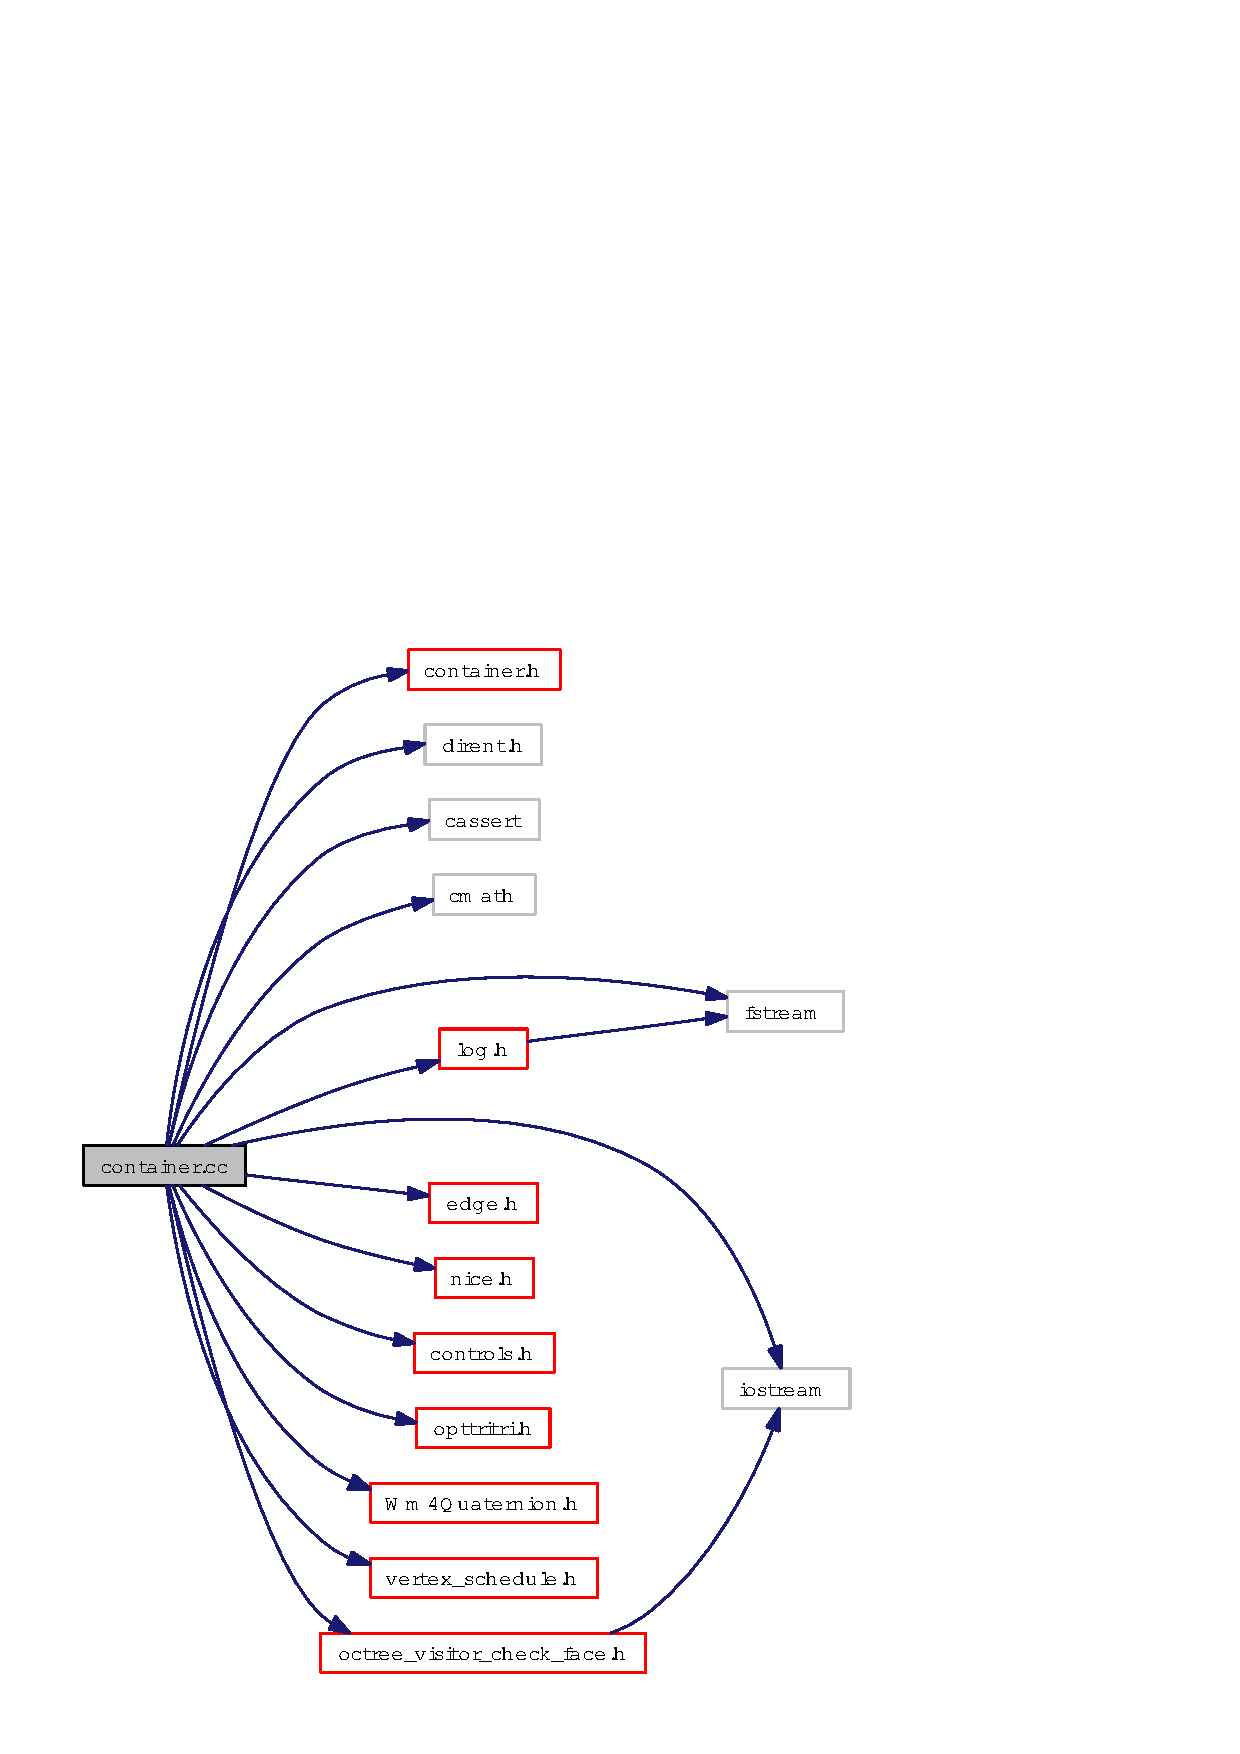
\includegraphics[width=206pt]{container_8cc__incl}
\end{center}
\end{figure}
\subsection*{Functions}
\begin{CompactItemize}
\item 
void {\bf keep\-Min} ({\bf vector3} \&min, {\bf Wm4::Vector3}$<$ double $>$ q)
\item 
void {\bf keep\-Max} ({\bf vector3} \&max, {\bf Wm4::Vector3}$<$ double $>$ q)
\end{CompactItemize}


\subsection{Function Documentation}
\index{container.cc@{container.cc}!keepMax@{keepMax}}
\index{keepMax@{keepMax}!container.cc@{container.cc}}
\subsubsection{\setlength{\rightskip}{0pt plus 5cm}void keep\-Max ({\bf vector3} \& {\em max}, {\bf Wm4::Vector3}$<$ double $>$ {\em q})}\label{container_8cc_751c0c375dacc25e2bab815b767b3fb6}


\index{container.cc@{container.cc}!keepMin@{keepMin}}
\index{keepMin@{keepMin}!container.cc@{container.cc}}
\subsubsection{\setlength{\rightskip}{0pt plus 5cm}void keep\-Min ({\bf vector3} \& {\em min}, {\bf Wm4::Vector3}$<$ double $>$ {\em q})}\label{container_8cc_4ad0271730b851c04d73a2438d7730da}



\hypertarget{container_8h}{
\section{container.h File Reference}
\label{container_8h}\index{container.h@{container.h}}
}
{\tt \#include $<$vector$>$}\par
{\tt \#include \char`\"{}object.h\char`\"{}}\par
\subsection*{Classes}
\begin{CompactItemize}
\item 
class \hyperlink{classContainer}{Container}
\end{CompactItemize}
\subsection*{Defines}
\begin{CompactItemize}
\item 
\#define \hyperlink{container_8h_6c0e07fabcd28953ed38855dfb61763c}{CONTAINER\_\-H}~1
\end{CompactItemize}
\subsection*{Typedefs}
\begin{CompactItemize}
\item 
typedef std::vector$<$ \hyperlink{classObject}{Object} $>$::iterator \hyperlink{container_8h_b1419b33b75b9fdefb8af198aca79708}{o\_\-iterator}
\item 
typedef std::vector$<$ \hyperlink{classObject}{Object} $>$::const\_\-iterator \hyperlink{container_8h_7f50282a208c7aa7c7af7b64b603ce61}{c\_\-o\_\-iterator}
\end{CompactItemize}


\subsection{Define Documentation}
\hypertarget{container_8h_6c0e07fabcd28953ed38855dfb61763c}{
\index{container.h@{container.h}!CONTAINER\_\-H@{CONTAINER\_\-H}}
\index{CONTAINER\_\-H@{CONTAINER\_\-H}!container.h@{container.h}}
\subsubsection[CONTAINER\_\-H]{\setlength{\rightskip}{0pt plus 5cm}\#define CONTAINER\_\-H~1}}
\label{container_8h_6c0e07fabcd28953ed38855dfb61763c}




\subsection{Typedef Documentation}
\hypertarget{container_8h_7f50282a208c7aa7c7af7b64b603ce61}{
\index{container.h@{container.h}!c\_\-o\_\-iterator@{c\_\-o\_\-iterator}}
\index{c\_\-o\_\-iterator@{c\_\-o\_\-iterator}!container.h@{container.h}}
\subsubsection[c\_\-o\_\-iterator]{\setlength{\rightskip}{0pt plus 5cm}typedef std::vector$<${\bf Object}$>$::const\_\-iterator {\bf c\_\-o\_\-iterator}}}
\label{container_8h_7f50282a208c7aa7c7af7b64b603ce61}


\hypertarget{container_8h_b1419b33b75b9fdefb8af198aca79708}{
\index{container.h@{container.h}!o\_\-iterator@{o\_\-iterator}}
\index{o\_\-iterator@{o\_\-iterator}!container.h@{container.h}}
\subsubsection[o\_\-iterator]{\setlength{\rightskip}{0pt plus 5cm}typedef std::vector$<${\bf Object}$>$::iterator {\bf o\_\-iterator}}}
\label{container_8h_b1419b33b75b9fdefb8af198aca79708}



\hypertarget{contour_8cc}{
\section{contour.cc File Reference}
\label{contour_8cc}\index{contour.cc@{contour.cc}}
}
{\tt \#include $<$algorithm$>$}\par
{\tt \#include $<$cassert$>$}\par
{\tt \#include $<$cmath$>$}\par
{\tt \#include $<$iostream$>$}\par
{\tt \#include $<$stdlib.h$>$}\par
{\tt \#include \char`\"{}contour.h\char`\"{}}\par
{\tt \#include \char`\"{}controls.h\char`\"{}}\par
{\tt \#include \char`\"{}control\_\-points.h\char`\"{}}\par
{\tt \#include \char`\"{}histogram.h\char`\"{}}\par
{\tt \#include \char`\"{}point.h\char`\"{}}\par
\subsection*{Variables}
\begin{CompactItemize}
\item 
const double \hyperlink{contour_8cc_08bbdb7f5f5c58271fb0ccdc450305f5}{spline\_\-ratio}
\end{CompactItemize}


\subsection{Variable Documentation}
\hypertarget{contour_8cc_08bbdb7f5f5c58271fb0ccdc450305f5}{
\index{contour.cc@{contour.cc}!spline\_\-ratio@{spline\_\-ratio}}
\index{spline\_\-ratio@{spline\_\-ratio}!contour.cc@{contour.cc}}
\subsubsection[spline\_\-ratio]{\setlength{\rightskip}{0pt plus 5cm}const double {\bf spline\_\-ratio}}}
\label{contour_8cc_08bbdb7f5f5c58271fb0ccdc450305f5}



\hypertarget{contour_8h}{
\section{contour.h File Reference}
\label{contour_8h}\index{contour.h@{contour.h}}
}
{\tt \#include $<$iostream$>$}\par
{\tt \#include $<$string$>$}\par
{\tt \#include $<$vector$>$}\par
{\tt \#include \char`\"{}control\_\-points.h\char`\"{}}\par
{\tt \#include \char`\"{}histogram.h\char`\"{}}\par
{\tt \#include \char`\"{}parameter.h\char`\"{}}\par
{\tt \#include \char`\"{}point.h\char`\"{}}\par
{\tt \#include \char`\"{}sim\_\-anneal.h\char`\"{}}\par
\subsection*{Classes}
\begin{CompactItemize}
\item 
class \hyperlink{classContour}{Contour}
\end{CompactItemize}
\subsection*{Defines}
\begin{CompactItemize}
\item 
\#define \hyperlink{contour_8h_1be3b74bacc91093c88d7dcef4ad7dae}{CONTOUR\_\-H}~1
\end{CompactItemize}
\subsection*{Typedefs}
\begin{CompactItemize}
\item 
typedef std::vector$<$ int $>$ \hyperlink{contour_8h_e59925ac43f8978cf3501e93cf1c098d}{vec\_\-i}
\item 
typedef std::vector$<$ int $>$::iterator \hyperlink{contour_8h_103f3d784284986bd2e813ac3fcc2ebe}{v\_\-i\_\-iterator}
\item 
typedef std::vector$<$ int $>$::const\_\-iterator \hyperlink{contour_8h_2f1f68221585603e5d4569fb0cd2f94a}{c\_\-v\_\-i\_\-iterator}
\item 
typedef std::vector$<$ int $>$::const\_\-reverse\_\-iterator \hyperlink{contour_8h_399d38bd867f2eab3cc38ccd9cdde360}{c\_\-r\_\-v\_\-i\_\-iterator}
\item 
typedef std::vector$<$ double $>$ \hyperlink{contour_8h_db0ab3db1ab685e2d2bff657e3e86861}{vec\_\-d}
\item 
typedef std::vector$<$ double $>$::iterator \hyperlink{contour_8h_a66ef4117b0ef362e6fbadb237199f05}{d\_\-iterator}
\item 
typedef std::vector$<$ double $>$::const\_\-iterator \hyperlink{contour_8h_76617663fb8c2b14cf698a47a4d07926}{c\_\-d\_\-iterator}
\item 
typedef std::vector$<$ \hyperlink{classPoint}{Point} $>$::iterator \hyperlink{contour_8h_bdc29b2296c12c432b5185786799144e}{p\_\-iterator}
\item 
typedef std::vector$<$ \hyperlink{classPoint}{Point} $>$::const\_\-iterator \hyperlink{contour_8h_d367c52cb5a031e4bc21ba9af7d6ee47}{c\_\-p\_\-iterator}
\item 
typedef std::list$<$ int $>$ \hyperlink{contour_8h_48cca362cb388dfdb3f8df5441d03717}{list\_\-i}
\item 
typedef std::list$<$ int $>$::iterator \hyperlink{contour_8h_c7559b6954586e2a7e87f9d34c211f15}{i\_\-iterator}
\end{CompactItemize}


\subsection{Define Documentation}
\hypertarget{contour_8h_1be3b74bacc91093c88d7dcef4ad7dae}{
\index{contour.h@{contour.h}!CONTOUR\_\-H@{CONTOUR\_\-H}}
\index{CONTOUR\_\-H@{CONTOUR\_\-H}!contour.h@{contour.h}}
\subsubsection[CONTOUR\_\-H]{\setlength{\rightskip}{0pt plus 5cm}\#define CONTOUR\_\-H~1}}
\label{contour_8h_1be3b74bacc91093c88d7dcef4ad7dae}




\subsection{Typedef Documentation}
\hypertarget{contour_8h_76617663fb8c2b14cf698a47a4d07926}{
\index{contour.h@{contour.h}!c\_\-d\_\-iterator@{c\_\-d\_\-iterator}}
\index{c\_\-d\_\-iterator@{c\_\-d\_\-iterator}!contour.h@{contour.h}}
\subsubsection[c\_\-d\_\-iterator]{\setlength{\rightskip}{0pt plus 5cm}typedef std::vector$<$double$>$::const\_\-iterator {\bf c\_\-d\_\-iterator}}}
\label{contour_8h_76617663fb8c2b14cf698a47a4d07926}


\hypertarget{contour_8h_d367c52cb5a031e4bc21ba9af7d6ee47}{
\index{contour.h@{contour.h}!c\_\-p\_\-iterator@{c\_\-p\_\-iterator}}
\index{c\_\-p\_\-iterator@{c\_\-p\_\-iterator}!contour.h@{contour.h}}
\subsubsection[c\_\-p\_\-iterator]{\setlength{\rightskip}{0pt plus 5cm}typedef std::vector$<${\bf Point}$>$::const\_\-iterator {\bf c\_\-p\_\-iterator}}}
\label{contour_8h_d367c52cb5a031e4bc21ba9af7d6ee47}


\hypertarget{contour_8h_399d38bd867f2eab3cc38ccd9cdde360}{
\index{contour.h@{contour.h}!c\_\-r\_\-v\_\-i\_\-iterator@{c\_\-r\_\-v\_\-i\_\-iterator}}
\index{c\_\-r\_\-v\_\-i\_\-iterator@{c\_\-r\_\-v\_\-i\_\-iterator}!contour.h@{contour.h}}
\subsubsection[c\_\-r\_\-v\_\-i\_\-iterator]{\setlength{\rightskip}{0pt plus 5cm}typedef std::vector$<$int$>$::const\_\-reverse\_\-iterator {\bf c\_\-r\_\-v\_\-i\_\-iterator}}}
\label{contour_8h_399d38bd867f2eab3cc38ccd9cdde360}


\hypertarget{contour_8h_2f1f68221585603e5d4569fb0cd2f94a}{
\index{contour.h@{contour.h}!c\_\-v\_\-i\_\-iterator@{c\_\-v\_\-i\_\-iterator}}
\index{c\_\-v\_\-i\_\-iterator@{c\_\-v\_\-i\_\-iterator}!contour.h@{contour.h}}
\subsubsection[c\_\-v\_\-i\_\-iterator]{\setlength{\rightskip}{0pt plus 5cm}typedef std::vector$<$int$>$::const\_\-iterator {\bf c\_\-v\_\-i\_\-iterator}}}
\label{contour_8h_2f1f68221585603e5d4569fb0cd2f94a}


\hypertarget{contour_8h_a66ef4117b0ef362e6fbadb237199f05}{
\index{contour.h@{contour.h}!d\_\-iterator@{d\_\-iterator}}
\index{d\_\-iterator@{d\_\-iterator}!contour.h@{contour.h}}
\subsubsection[d\_\-iterator]{\setlength{\rightskip}{0pt plus 5cm}typedef std::vector$<$double$>$::iterator {\bf d\_\-iterator}}}
\label{contour_8h_a66ef4117b0ef362e6fbadb237199f05}


\hypertarget{contour_8h_c7559b6954586e2a7e87f9d34c211f15}{
\index{contour.h@{contour.h}!i\_\-iterator@{i\_\-iterator}}
\index{i\_\-iterator@{i\_\-iterator}!contour.h@{contour.h}}
\subsubsection[i\_\-iterator]{\setlength{\rightskip}{0pt plus 5cm}typedef std::list$<$int$>$::iterator {\bf i\_\-iterator}}}
\label{contour_8h_c7559b6954586e2a7e87f9d34c211f15}


\hypertarget{contour_8h_48cca362cb388dfdb3f8df5441d03717}{
\index{contour.h@{contour.h}!list\_\-i@{list\_\-i}}
\index{list\_\-i@{list\_\-i}!contour.h@{contour.h}}
\subsubsection[list\_\-i]{\setlength{\rightskip}{0pt plus 5cm}typedef std::list$<$int$>$ {\bf list\_\-i}}}
\label{contour_8h_48cca362cb388dfdb3f8df5441d03717}


\hypertarget{contour_8h_bdc29b2296c12c432b5185786799144e}{
\index{contour.h@{contour.h}!p\_\-iterator@{p\_\-iterator}}
\index{p\_\-iterator@{p\_\-iterator}!contour.h@{contour.h}}
\subsubsection[p\_\-iterator]{\setlength{\rightskip}{0pt plus 5cm}typedef std::vector$<${\bf Point}$>$::iterator {\bf p\_\-iterator}}}
\label{contour_8h_bdc29b2296c12c432b5185786799144e}


\hypertarget{contour_8h_103f3d784284986bd2e813ac3fcc2ebe}{
\index{contour.h@{contour.h}!v\_\-i\_\-iterator@{v\_\-i\_\-iterator}}
\index{v\_\-i\_\-iterator@{v\_\-i\_\-iterator}!contour.h@{contour.h}}
\subsubsection[v\_\-i\_\-iterator]{\setlength{\rightskip}{0pt plus 5cm}typedef std::vector$<$int$>$::iterator {\bf v\_\-i\_\-iterator}}}
\label{contour_8h_103f3d784284986bd2e813ac3fcc2ebe}


\hypertarget{contour_8h_db0ab3db1ab685e2d2bff657e3e86861}{
\index{contour.h@{contour.h}!vec\_\-d@{vec\_\-d}}
\index{vec\_\-d@{vec\_\-d}!contour.h@{contour.h}}
\subsubsection[vec\_\-d]{\setlength{\rightskip}{0pt plus 5cm}typedef std::vector$<$double$>$ {\bf vec\_\-d}}}
\label{contour_8h_db0ab3db1ab685e2d2bff657e3e86861}


\hypertarget{contour_8h_e59925ac43f8978cf3501e93cf1c098d}{
\index{contour.h@{contour.h}!vec\_\-i@{vec\_\-i}}
\index{vec\_\-i@{vec\_\-i}!contour.h@{contour.h}}
\subsubsection[vec\_\-i]{\setlength{\rightskip}{0pt plus 5cm}typedef std::vector$<$int$>$ {\bf vec\_\-i}}}
\label{contour_8h_e59925ac43f8978cf3501e93cf1c098d}



\hypertarget{control__points_8cc}{
\section{control\_\-points.cc File Reference}
\label{control__points_8cc}\index{control\_\-points.cc@{control\_\-points.cc}}
}
{\tt \#include \char`\"{}contour.h\char`\"{}}\par
{\tt \#include \char`\"{}control\_\-points.h\char`\"{}}\par

\hypertarget{control__points_8h}{
\section{control\_\-points.h File Reference}
\label{control__points_8h}\index{control\_\-points.h@{control\_\-points.h}}
}
{\tt \#include $<$cassert$>$}\par
{\tt \#include $<$list$>$}\par
{\tt \#include \char`\"{}controls.h\char`\"{}}\par
\subsection*{Classes}
\begin{CompactItemize}
\item 
class \hyperlink{classControl__Points}{Control\_\-Points}
\end{CompactItemize}
\subsection*{Defines}
\begin{CompactItemize}
\item 
\#define \hyperlink{control__points_8h_5a585c2809dc60c2d64ada437dec1dab}{CONTROL\_\-POINTS\_\-H}~1
\end{CompactItemize}


\subsection{Define Documentation}
\hypertarget{control__points_8h_5a585c2809dc60c2d64ada437dec1dab}{
\index{control\_\-points.h@{control\_\-points.h}!CONTROL\_\-POINTS\_\-H@{CONTROL\_\-POINTS\_\-H}}
\index{CONTROL\_\-POINTS\_\-H@{CONTROL\_\-POINTS\_\-H}!control_points.h@{control\_\-points.h}}
\subsubsection[CONTROL\_\-POINTS\_\-H]{\setlength{\rightskip}{0pt plus 5cm}\#define CONTROL\_\-POINTS\_\-H~1}}
\label{control__points_8h_5a585c2809dc60c2d64ada437dec1dab}



\section{controls.cc File Reference}
\label{controls_8cc}\index{controls.cc@{controls.cc}}
{\tt \#include \char`\"{}controls.h\char`\"{}}\par
{\tt \#include $<$iostream$>$}\par
{\tt \#include $<$getopt.h$>$}\par
{\tt \#include $<$cmath$>$}\par
{\tt \#include \char`\"{}container.h\char`\"{}}\par


Include dependency graph for controls.cc:\begin{figure}[H]
\begin{center}
\leavevmode
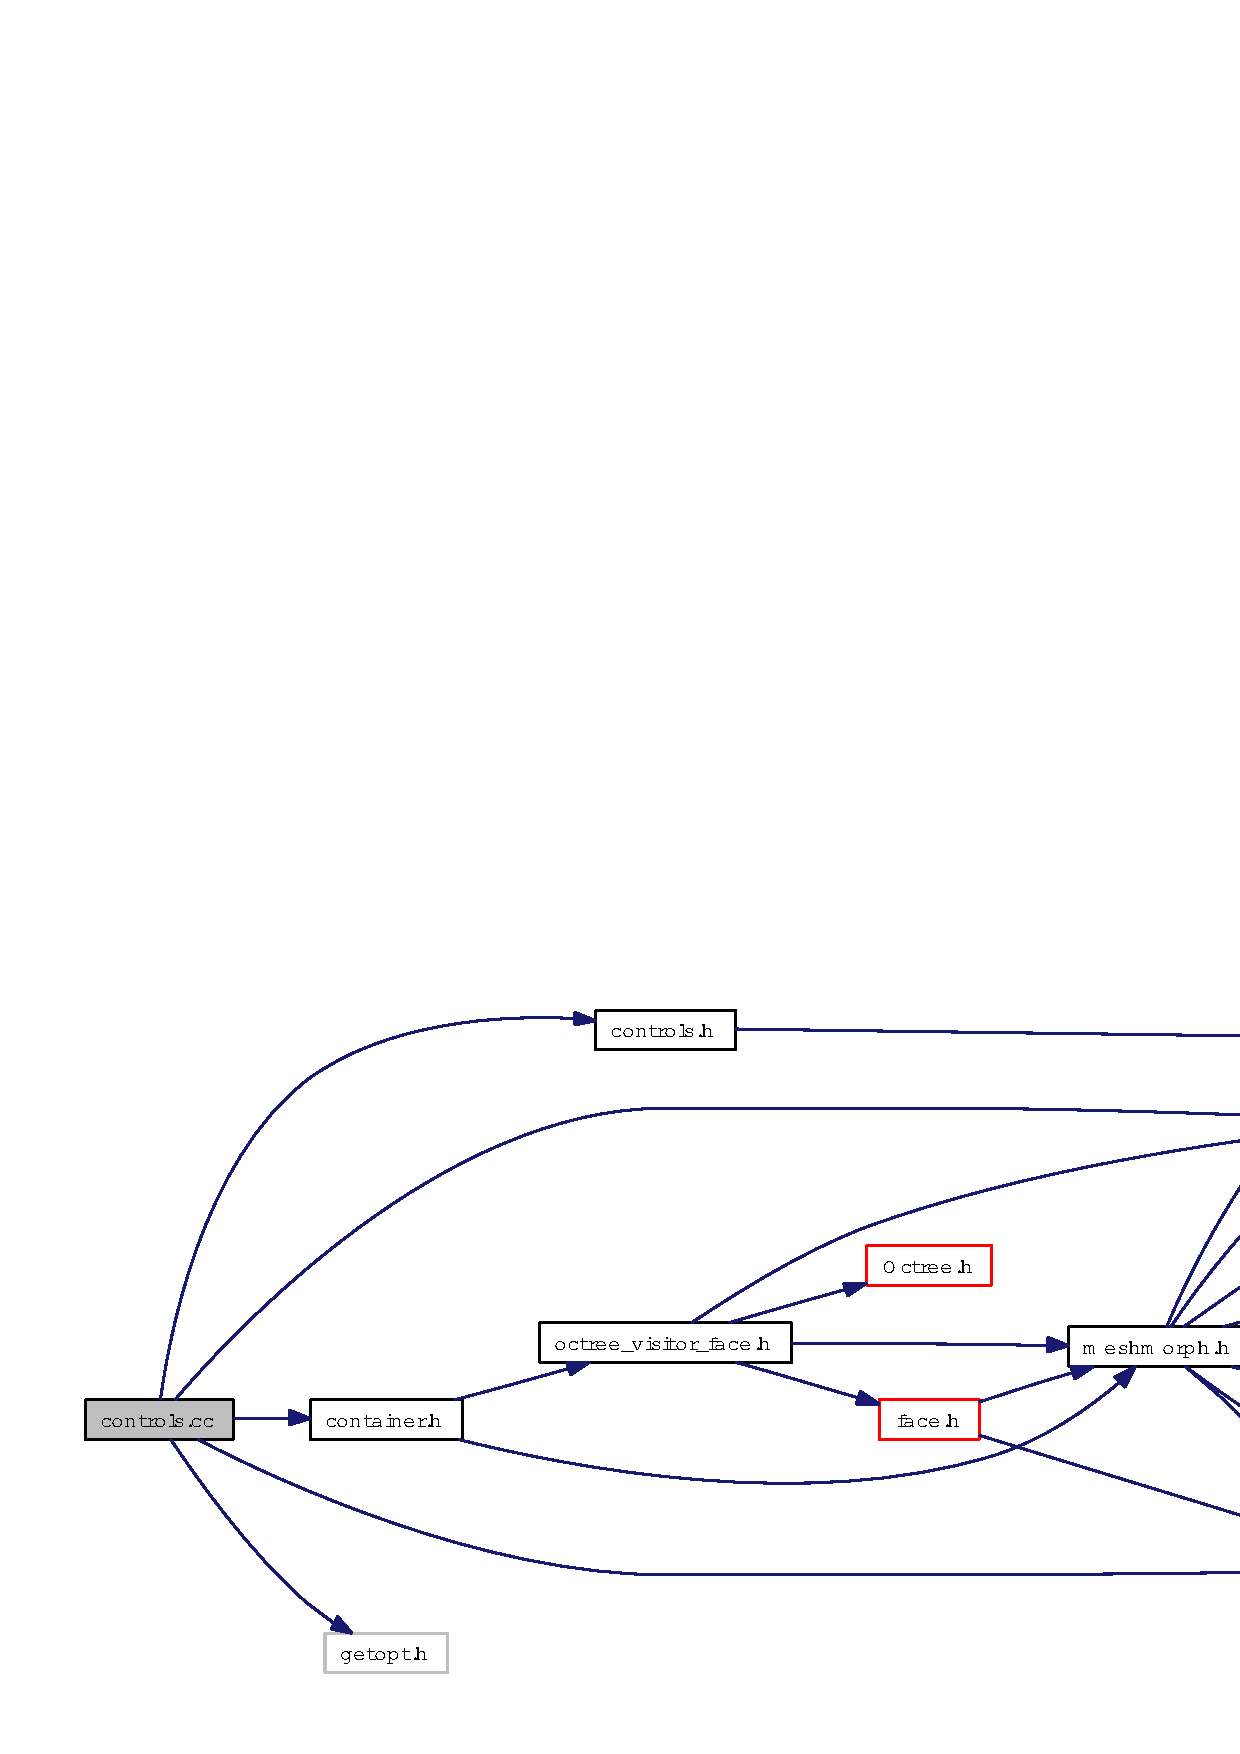
\includegraphics[width=364pt]{controls_8cc__incl}
\end{center}
\end{figure}

\hypertarget{controls_8h}{
\section{controls.h File Reference}
\label{controls_8h}\index{controls.h@{controls.h}}
}
{\tt \#include $<$cassert$>$}\par
{\tt \#include $<$getopt.h$>$}\par
{\tt \#include $<$string.h$>$}\par
{\tt \#include $<$string$>$}\par
{\tt \#include $<$vector$>$}\par
\subsection*{Classes}
\begin{CompactItemize}
\item 
class \hyperlink{classControls}{Controls}
\end{CompactItemize}
\subsection*{Defines}
\begin{CompactItemize}
\item 
\#define \hyperlink{controls_8h_dbcef44a41ba27e50a21d80a826bcf1e}{CONTROLS\_\-H}~1
\end{CompactItemize}


\subsection{Define Documentation}
\hypertarget{controls_8h_dbcef44a41ba27e50a21d80a826bcf1e}{
\index{controls.h@{controls.h}!CONTROLS\_\-H@{CONTROLS\_\-H}}
\index{CONTROLS\_\-H@{CONTROLS\_\-H}!controls.h@{controls.h}}
\subsubsection[CONTROLS\_\-H]{\setlength{\rightskip}{0pt plus 5cm}\#define CONTROLS\_\-H~1}}
\label{controls_8h_dbcef44a41ba27e50a21d80a826bcf1e}



\hypertarget{histogram_8cc}{
\section{histogram.cc File Reference}
\label{histogram_8cc}\index{histogram.cc@{histogram.cc}}
}
{\tt \#include $<$iostream$>$}\par
{\tt \#include \char`\"{}histogram.h\char`\"{}}\par
{\tt \#include \char`\"{}contour.h\char`\"{}}\par
\subsection*{Variables}
\begin{CompactItemize}
\item 
const int \hyperlink{histogram_8cc_b2c3002d9c147ccab84d3a8c061d6a06}{num\_\-bins}
\end{CompactItemize}


\subsection{Variable Documentation}
\hypertarget{histogram_8cc_b2c3002d9c147ccab84d3a8c061d6a06}{
\index{histogram.cc@{histogram.cc}!num\_\-bins@{num\_\-bins}}
\index{num\_\-bins@{num\_\-bins}!histogram.cc@{histogram.cc}}
\subsubsection[num\_\-bins]{\setlength{\rightskip}{0pt plus 5cm}const int {\bf num\_\-bins}}}
\label{histogram_8cc_b2c3002d9c147ccab84d3a8c061d6a06}



\hypertarget{histogram_8h}{
\section{histogram.h File Reference}
\label{histogram_8h}\index{histogram.h@{histogram.h}}
}
{\tt \#include $<$iostream$>$}\par
{\tt \#include \char`\"{}reconstruct2contourtiler.h\char`\"{}}\par
\subsection*{Classes}
\begin{CompactItemize}
\item 
class \hyperlink{classHistogram}{Histogram}
\end{CompactItemize}
\subsection*{Defines}
\begin{CompactItemize}
\item 
\#define \hyperlink{histogram_8h_10d749b7e9d09f11fb1dd266c6168a5a}{HISTOGRAM\_\-H}~1
\end{CompactItemize}
\subsection*{Typedefs}
\begin{CompactItemize}
\item 
typedef std::vector$<$ double $>$ \hyperlink{histogram_8h_db0ab3db1ab685e2d2bff657e3e86861}{vec\_\-d}
\item 
typedef std::vector$<$ double $>$::iterator \hyperlink{histogram_8h_a66ef4117b0ef362e6fbadb237199f05}{d\_\-iterator}
\item 
typedef std::vector$<$ double $>$::const\_\-iterator \hyperlink{histogram_8h_76617663fb8c2b14cf698a47a4d07926}{c\_\-d\_\-iterator}
\end{CompactItemize}


\subsection{Define Documentation}
\hypertarget{histogram_8h_10d749b7e9d09f11fb1dd266c6168a5a}{
\index{histogram.h@{histogram.h}!HISTOGRAM\_\-H@{HISTOGRAM\_\-H}}
\index{HISTOGRAM\_\-H@{HISTOGRAM\_\-H}!histogram.h@{histogram.h}}
\subsubsection[HISTOGRAM\_\-H]{\setlength{\rightskip}{0pt plus 5cm}\#define HISTOGRAM\_\-H~1}}
\label{histogram_8h_10d749b7e9d09f11fb1dd266c6168a5a}




\subsection{Typedef Documentation}
\hypertarget{histogram_8h_76617663fb8c2b14cf698a47a4d07926}{
\index{histogram.h@{histogram.h}!c\_\-d\_\-iterator@{c\_\-d\_\-iterator}}
\index{c\_\-d\_\-iterator@{c\_\-d\_\-iterator}!histogram.h@{histogram.h}}
\subsubsection[c\_\-d\_\-iterator]{\setlength{\rightskip}{0pt plus 5cm}typedef std::vector$<$double$>$::const\_\-iterator {\bf c\_\-d\_\-iterator}}}
\label{histogram_8h_76617663fb8c2b14cf698a47a4d07926}


\hypertarget{histogram_8h_a66ef4117b0ef362e6fbadb237199f05}{
\index{histogram.h@{histogram.h}!d\_\-iterator@{d\_\-iterator}}
\index{d\_\-iterator@{d\_\-iterator}!histogram.h@{histogram.h}}
\subsubsection[d\_\-iterator]{\setlength{\rightskip}{0pt plus 5cm}typedef std::vector$<$double$>$::iterator {\bf d\_\-iterator}}}
\label{histogram_8h_a66ef4117b0ef362e6fbadb237199f05}


\hypertarget{histogram_8h_db0ab3db1ab685e2d2bff657e3e86861}{
\index{histogram.h@{histogram.h}!vec\_\-d@{vec\_\-d}}
\index{vec\_\-d@{vec\_\-d}!histogram.h@{histogram.h}}
\subsubsection[vec\_\-d]{\setlength{\rightskip}{0pt plus 5cm}typedef std::vector$<$double$>$ {\bf vec\_\-d}}}
\label{histogram_8h_db0ab3db1ab685e2d2bff657e3e86861}



\hypertarget{object_8cc}{
\section{object.cc File Reference}
\label{object_8cc}\index{object.cc@{object.cc}}
}
{\tt \#include $<$iostream$>$}\par
{\tt \#include $<$string$>$}\par
{\tt \#include $<$stdlib.h$>$}\par
{\tt \#include \char`\"{}contour.h\char`\"{}}\par
{\tt \#include \char`\"{}controls.h\char`\"{}}\par
{\tt \#include \char`\"{}object.h\char`\"{}}\par

\section{object.h File Reference}
\label{object_8h}\index{object.h@{object.h}}
{\tt \#include \char`\"{}meshmorph.h\char`\"{}}\par


Include dependency graph for object.h:\begin{figure}[H]
\begin{center}
\leavevmode
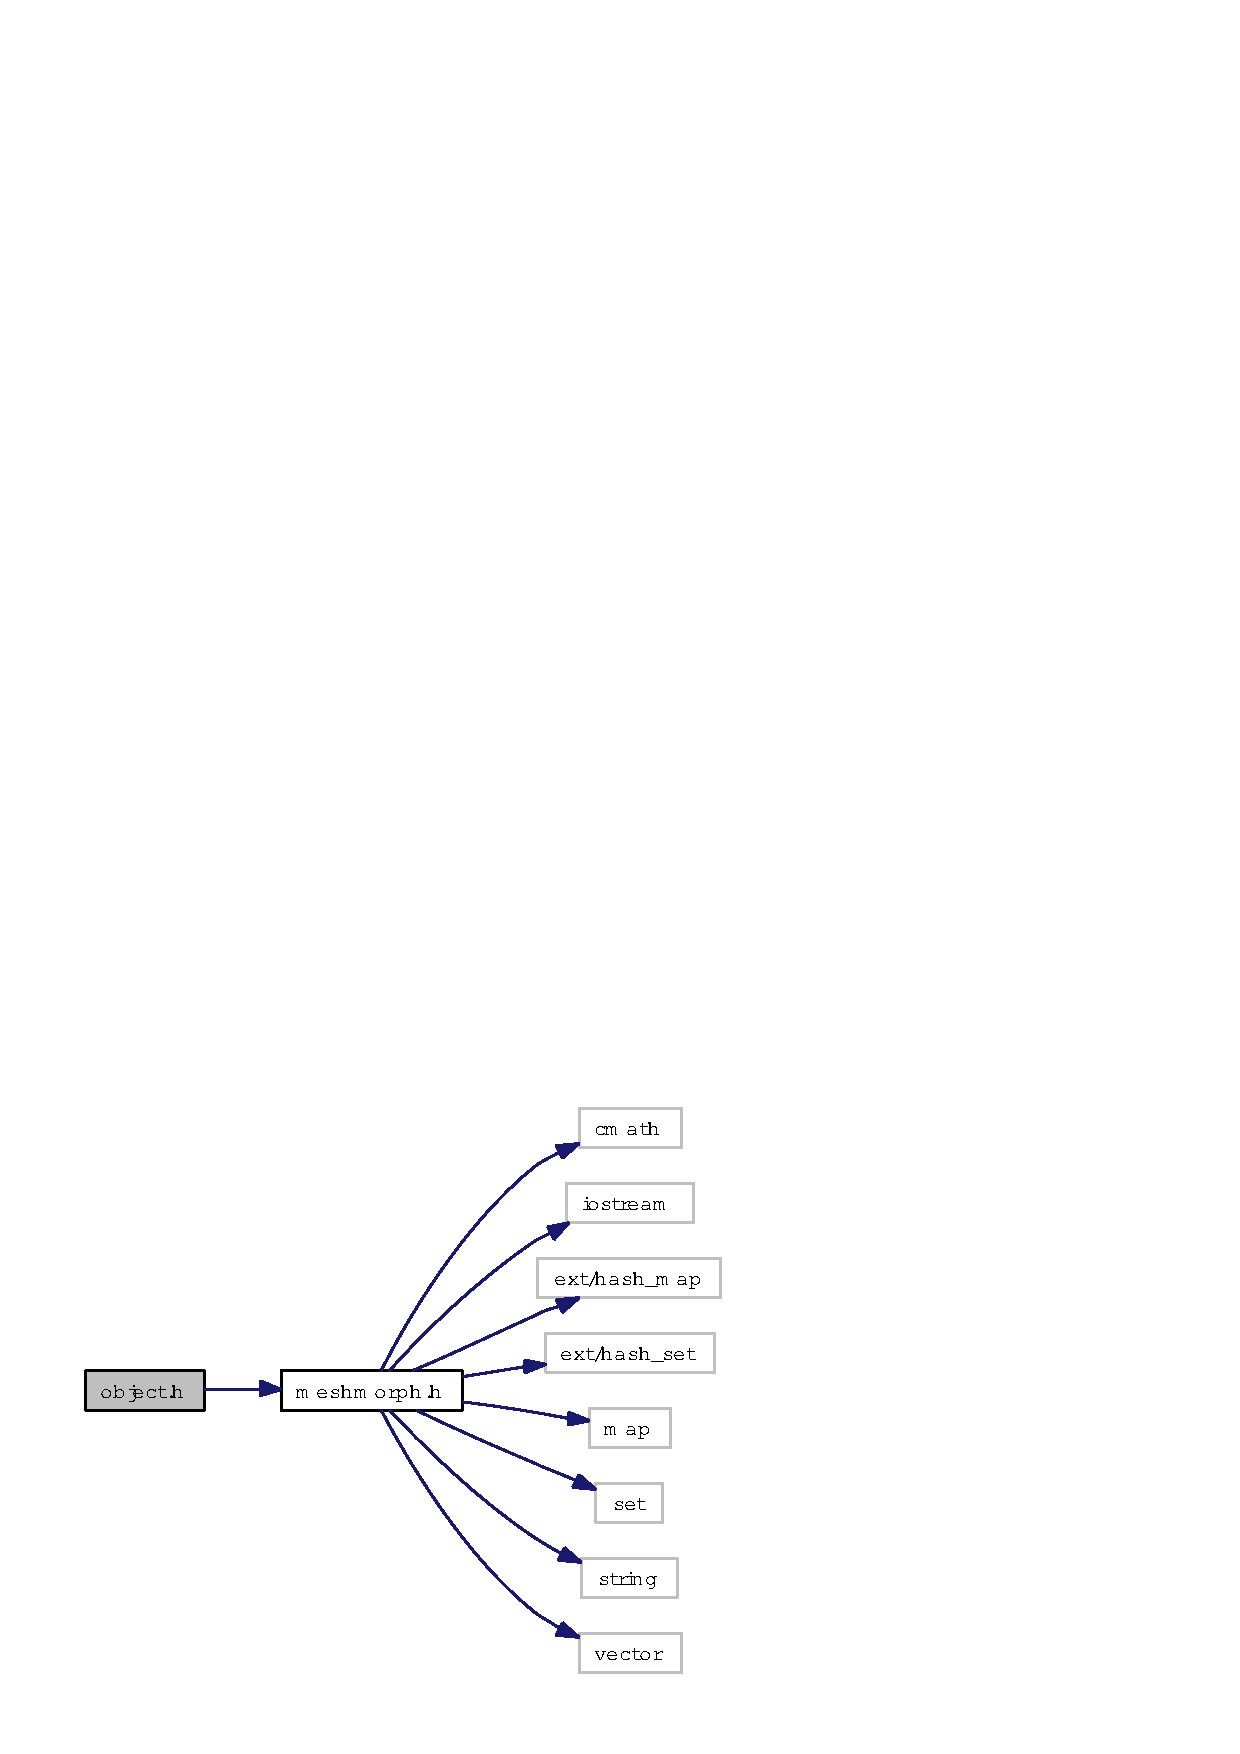
\includegraphics[width=175pt]{object_8h__incl}
\end{center}
\end{figure}


This graph shows which files directly or indirectly include this file:\begin{figure}[H]
\begin{center}
\leavevmode
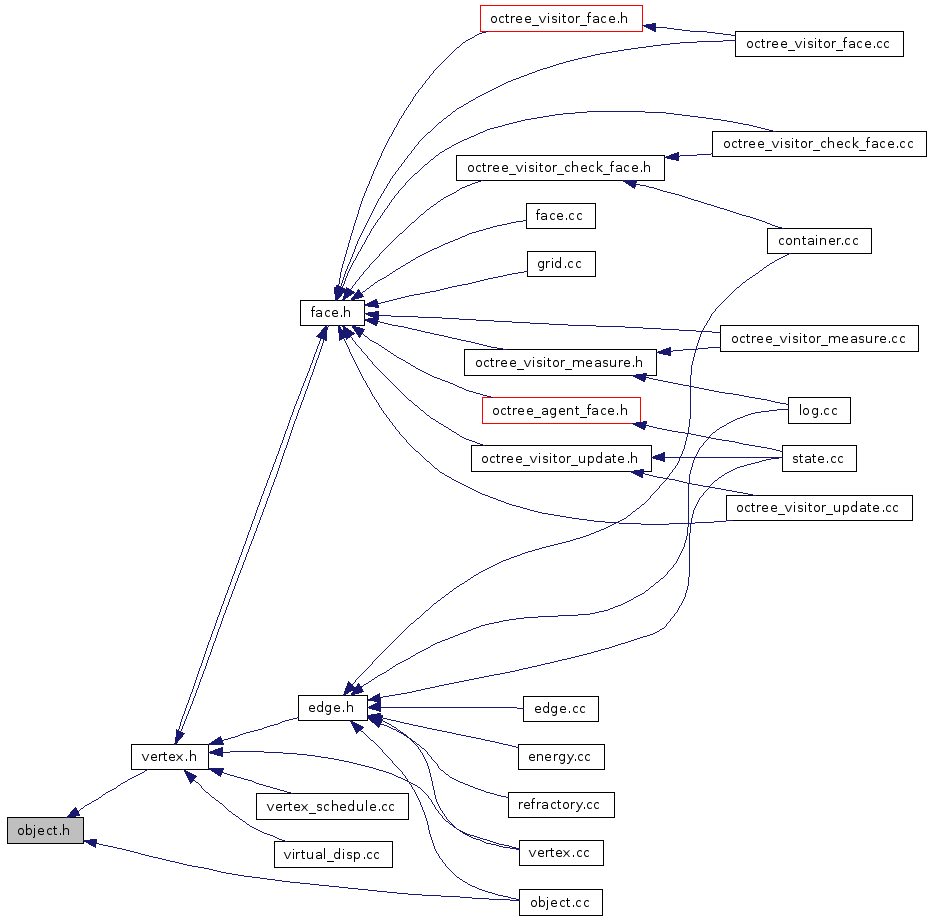
\includegraphics[width=367pt]{object_8h__dep__incl}
\end{center}
\end{figure}
\subsection*{Classes}
\begin{CompactItemize}
\item 
class {\bf Object}
\end{CompactItemize}
\subsection*{Defines}
\begin{CompactItemize}
\item 
\#define {\bf OBJECT\_\-H}~1
\end{CompactItemize}
\subsection*{Typedefs}
\begin{CompactItemize}
\item 
typedef std::map$<$ std::string, {\bf Edge} $\ast$, {\bf lts} $>$::const\_\-iterator {\bf msep\_\-cit}
\end{CompactItemize}


\subsection{Define Documentation}
\index{object.h@{object.h}!OBJECT_H@{OBJECT\_\-H}}
\index{OBJECT_H@{OBJECT\_\-H}!object.h@{object.h}}
\subsubsection{\setlength{\rightskip}{0pt plus 5cm}\#define OBJECT\_\-H~1}\label{object_8h_a8010467994983b5e7d22edee6ab6806}




\subsection{Typedef Documentation}
\index{object.h@{object.h}!msep_cit@{msep\_\-cit}}
\index{msep_cit@{msep\_\-cit}!object.h@{object.h}}
\subsubsection{\setlength{\rightskip}{0pt plus 5cm}typedef std::map$<$std::string,{\bf Edge}$\ast$,{\bf lts}$>$::const\_\-iterator {\bf msep\_\-cit}}\label{object_8h_0b55971f5102e117df638ddc4acd0182}



\hypertarget{parameter_8cc}{
\section{parameter.cc File Reference}
\label{parameter_8cc}\index{parameter.cc@{parameter.cc}}
}
{\tt \#include $<$algorithm$>$}\par
{\tt \#include $<$cmath$>$}\par
{\tt \#include $<$iostream$>$}\par
{\tt \#include $<$string$>$}\par
{\tt \#include \char`\"{}parameter.h\char`\"{}}\par
{\tt \#include \char`\"{}controls.h\char`\"{}}\par

\hypertarget{parameter_8h}{
\section{parameter.h File Reference}
\label{parameter_8h}\index{parameter.h@{parameter.h}}
}
{\tt \#include $<$cassert$>$}\par
{\tt \#include $<$vector$>$}\par
{\tt \#include \char`\"{}controls.h\char`\"{}}\par
{\tt \#include \char`\"{}point.h\char`\"{}}\par
\subsection*{Classes}
\begin{CompactItemize}
\item 
class \hyperlink{classParameter}{Parameter}
\end{CompactItemize}
\subsection*{Defines}
\begin{CompactItemize}
\item 
\#define \hyperlink{parameter_8h_a59b26b199c29b4c9319323a28bdef0e}{PARAMETER\_\-H}~1
\end{CompactItemize}
\subsection*{Typedefs}
\begin{CompactItemize}
\item 
typedef std::vector$<$ \hyperlink{classPoint}{Point} $>$ \hyperlink{parameter_8h_0f255c18b931c840fa6b8a911473da92}{vec\_\-p}
\item 
typedef std::vector$<$ \hyperlink{classPoint}{Point} $>$::iterator \hyperlink{parameter_8h_bdc29b2296c12c432b5185786799144e}{p\_\-iterator}
\item 
typedef std::vector$<$ \hyperlink{classPoint}{Point} $>$::const\_\-iterator \hyperlink{parameter_8h_d367c52cb5a031e4bc21ba9af7d6ee47}{c\_\-p\_\-iterator}
\item 
typedef std::vector$<$ double $>$::const\_\-iterator \hyperlink{parameter_8h_76617663fb8c2b14cf698a47a4d07926}{c\_\-d\_\-iterator}
\item 
typedef std::vector$<$ int $>$ \hyperlink{parameter_8h_e59925ac43f8978cf3501e93cf1c098d}{vec\_\-i}
\end{CompactItemize}


\subsection{Define Documentation}
\hypertarget{parameter_8h_a59b26b199c29b4c9319323a28bdef0e}{
\index{parameter.h@{parameter.h}!PARAMETER\_\-H@{PARAMETER\_\-H}}
\index{PARAMETER\_\-H@{PARAMETER\_\-H}!parameter.h@{parameter.h}}
\subsubsection[PARAMETER\_\-H]{\setlength{\rightskip}{0pt plus 5cm}\#define PARAMETER\_\-H~1}}
\label{parameter_8h_a59b26b199c29b4c9319323a28bdef0e}




\subsection{Typedef Documentation}
\hypertarget{parameter_8h_76617663fb8c2b14cf698a47a4d07926}{
\index{parameter.h@{parameter.h}!c\_\-d\_\-iterator@{c\_\-d\_\-iterator}}
\index{c\_\-d\_\-iterator@{c\_\-d\_\-iterator}!parameter.h@{parameter.h}}
\subsubsection[c\_\-d\_\-iterator]{\setlength{\rightskip}{0pt plus 5cm}typedef std::vector$<$double$>$::const\_\-iterator {\bf c\_\-d\_\-iterator}}}
\label{parameter_8h_76617663fb8c2b14cf698a47a4d07926}


\hypertarget{parameter_8h_d367c52cb5a031e4bc21ba9af7d6ee47}{
\index{parameter.h@{parameter.h}!c\_\-p\_\-iterator@{c\_\-p\_\-iterator}}
\index{c\_\-p\_\-iterator@{c\_\-p\_\-iterator}!parameter.h@{parameter.h}}
\subsubsection[c\_\-p\_\-iterator]{\setlength{\rightskip}{0pt plus 5cm}typedef std::vector$<${\bf Point}$>$::const\_\-iterator {\bf c\_\-p\_\-iterator}}}
\label{parameter_8h_d367c52cb5a031e4bc21ba9af7d6ee47}


\hypertarget{parameter_8h_bdc29b2296c12c432b5185786799144e}{
\index{parameter.h@{parameter.h}!p\_\-iterator@{p\_\-iterator}}
\index{p\_\-iterator@{p\_\-iterator}!parameter.h@{parameter.h}}
\subsubsection[p\_\-iterator]{\setlength{\rightskip}{0pt plus 5cm}typedef std::vector$<${\bf Point}$>$::iterator {\bf p\_\-iterator}}}
\label{parameter_8h_bdc29b2296c12c432b5185786799144e}


\hypertarget{parameter_8h_e59925ac43f8978cf3501e93cf1c098d}{
\index{parameter.h@{parameter.h}!vec\_\-i@{vec\_\-i}}
\index{vec\_\-i@{vec\_\-i}!parameter.h@{parameter.h}}
\subsubsection[vec\_\-i]{\setlength{\rightskip}{0pt plus 5cm}typedef std::vector$<$int$>$ {\bf vec\_\-i}}}
\label{parameter_8h_e59925ac43f8978cf3501e93cf1c098d}


\hypertarget{parameter_8h_0f255c18b931c840fa6b8a911473da92}{
\index{parameter.h@{parameter.h}!vec\_\-p@{vec\_\-p}}
\index{vec\_\-p@{vec\_\-p}!parameter.h@{parameter.h}}
\subsubsection[vec\_\-p]{\setlength{\rightskip}{0pt plus 5cm}typedef std::vector$<${\bf Point}$>$ {\bf vec\_\-p}}}
\label{parameter_8h_0f255c18b931c840fa6b8a911473da92}



\hypertarget{point_8cc}{
\section{point.cc File Reference}
\label{point_8cc}\index{point.cc@{point.cc}}
}
{\tt \#include $<$iostream$>$}\par
{\tt \#include $<$stdlib.h$>$}\par
{\tt \#include $<$string$>$}\par
{\tt \#include $<$string.h$>$}\par
{\tt \#include \char`\"{}point.h\char`\"{}}\par

\hypertarget{point_8h}{
\section{point.h File Reference}
\label{point_8h}\index{point.h@{point.h}}
}
{\tt \#include $<$math.h$>$}\par
{\tt \#include $<$stdio.h$>$}\par
\subsection*{Classes}
\begin{CompactItemize}
\item 
class \hyperlink{classPoint}{Point}
\end{CompactItemize}
\subsection*{Defines}
\begin{CompactItemize}
\item 
\#define \hyperlink{point_8h_b256d307f1a79781462e727dbf574870}{POINT\_\-H}~1
\end{CompactItemize}


\subsection{Define Documentation}
\hypertarget{point_8h_b256d307f1a79781462e727dbf574870}{
\index{point.h@{point.h}!POINT\_\-H@{POINT\_\-H}}
\index{POINT\_\-H@{POINT\_\-H}!point.h@{point.h}}
\subsubsection[POINT\_\-H]{\setlength{\rightskip}{0pt plus 5cm}\#define POINT\_\-H~1}}
\label{point_8h_b256d307f1a79781462e727dbf574870}



\hypertarget{reconstruct2contourtiler_8cc}{
\section{reconstruct2contourtiler.cc File Reference}
\label{reconstruct2contourtiler_8cc}\index{reconstruct2contourtiler.cc@{reconstruct2contourtiler.cc}}
}
{\tt \#include $<$stdlib.h$>$}\par
{\tt \#include $<$string$>$}\par
{\tt \#include $<$cmath$>$}\par
{\tt \#include \char`\"{}reconstruct2contourtiler.h\char`\"{}}\par
\subsection*{Functions}
\begin{CompactItemize}
\item 
int \hyperlink{reconstruct2contourtiler_8cc_0ddf1224851353fc92bfbff6f499fa97}{main} (int argc, char $\ast$argv\mbox{[}$\,$\mbox{]})
\item 
bool \hyperlink{reconstruct2contourtiler_8cc_54baf86f92ae2f215fbf2fc9d9913868}{distinguishable} (double \hyperlink{proximity__energy_8m_4124bc0a9335c27f086f24ba207a4912}{a}, double b, double epsilon)
\item 
bool \hyperlink{reconstruct2contourtiler_8cc_7e48ad73971e78bc20e3deb1e74546ad}{distinguishable} (double \hyperlink{proximity__energy_8m_4124bc0a9335c27f086f24ba207a4912}{a}, double b)
\end{CompactItemize}


\subsection{Function Documentation}
\hypertarget{reconstruct2contourtiler_8cc_7e48ad73971e78bc20e3deb1e74546ad}{
\index{reconstruct2contourtiler.cc@{reconstruct2contourtiler.cc}!distinguishable@{distinguishable}}
\index{distinguishable@{distinguishable}!reconstruct2contourtiler.cc@{reconstruct2contourtiler.cc}}
\subsubsection[distinguishable]{\setlength{\rightskip}{0pt plus 5cm}bool distinguishable (double {\em a}, \/  double {\em b})}}
\label{reconstruct2contourtiler_8cc_7e48ad73971e78bc20e3deb1e74546ad}


Determine if two floating-point precision numbers are equivalent in value within MY\_\-DOUBLE\_\-EPSILON. \begin{Desc}
\item[Parameters:]
\begin{description}
\item[\mbox{$\leftarrow$} {\em a}]First number. \item[\mbox{$\leftarrow$} {\em b}]Second number. \end{description}
\end{Desc}
\begin{Desc}
\item[Returns:]1 if Inputs are different; 0 otherwise. \end{Desc}


References distinguishable(), and Controls::instance().\hypertarget{reconstruct2contourtiler_8cc_54baf86f92ae2f215fbf2fc9d9913868}{
\index{reconstruct2contourtiler.cc@{reconstruct2contourtiler.cc}!distinguishable@{distinguishable}}
\index{distinguishable@{distinguishable}!reconstruct2contourtiler.cc@{reconstruct2contourtiler.cc}}
\subsubsection[distinguishable]{\setlength{\rightskip}{0pt plus 5cm}bool distinguishable (double {\em a}, \/  double {\em b}, \/  double {\em epsilon})}}
\label{reconstruct2contourtiler_8cc_54baf86f92ae2f215fbf2fc9d9913868}


Determine if two floating-point precision numbers are equivalent in value within epsilon. \begin{Desc}
\item[Parameters:]
\begin{description}
\item[\mbox{$\leftarrow$} {\em a}]First number. \item[\mbox{$\leftarrow$} {\em b}]Second number. \item[\mbox{$\leftarrow$} {\em epsilon}]The difference between the two input values must be greater than the fraction of the largest input value defined by epsilon. \end{description}
\end{Desc}
\begin{Desc}
\item[Returns:]1 if Inputs are different; 0 otherwise. \end{Desc}


Referenced by distinguishable().\hypertarget{reconstruct2contourtiler_8cc_0ddf1224851353fc92bfbff6f499fa97}{
\index{reconstruct2contourtiler.cc@{reconstruct2contourtiler.cc}!main@{main}}
\index{main@{main}!reconstruct2contourtiler.cc@{reconstruct2contourtiler.cc}}
\subsubsection[main]{\setlength{\rightskip}{0pt plus 5cm}int main (int {\em argc}, \/  char $\ast$ {\em argv}\mbox{[}$\,$\mbox{]})}}
\label{reconstruct2contourtiler_8cc_0ddf1224851353fc92bfbff6f499fa97}




References Container::clearOutputScripts(), Container::getContours(), Container::getNumContours(), Container::getNumFiles(), Container::getNumObjects(), Container::getNumRawPoints(), Controls::getPrintDetailedInfo(), Controls::instance(), Controls::parseCommandLine(), Container::printRawPoints(), Histogram::printStatistics(), Container::processContour(), Container::removeDuplicates(), and Container::writeOutputContours().
\hypertarget{reconstruct2contourtiler_8h}{
\section{reconstruct2contourtiler.h File Reference}
\label{reconstruct2contourtiler_8h}\index{reconstruct2contourtiler.h@{reconstruct2contourtiler.h}}
}
{\tt \#include $<$vector$>$}\par
{\tt \#include \char`\"{}container.h\char`\"{}}\par
{\tt \#include \char`\"{}controls.h\char`\"{}}\par
\subsection*{Defines}
\begin{CompactItemize}
\item 
\#define \hyperlink{reconstruct2contourtiler_8h_06fa45c9a07cb93acfd7b53235ef9103}{RECONSTRUCT2CONTOURTILER\_\-H}~1
\end{CompactItemize}
\subsection*{Functions}
\begin{CompactItemize}
\item 
bool \hyperlink{reconstruct2contourtiler_8h_54baf86f92ae2f215fbf2fc9d9913868}{distinguishable} (double a, double b, double epsilon)
\item 
bool \hyperlink{reconstruct2contourtiler_8h_7e48ad73971e78bc20e3deb1e74546ad}{distinguishable} (double a, double b)
\end{CompactItemize}


\subsection{Define Documentation}
\hypertarget{reconstruct2contourtiler_8h_06fa45c9a07cb93acfd7b53235ef9103}{
\index{reconstruct2contourtiler.h@{reconstruct2contourtiler.h}!RECONSTRUCT2CONTOURTILER\_\-H@{RECONSTRUCT2CONTOURTILER\_\-H}}
\index{RECONSTRUCT2CONTOURTILER\_\-H@{RECONSTRUCT2CONTOURTILER\_\-H}!reconstruct2contourtiler.h@{reconstruct2contourtiler.h}}
\subsubsection[RECONSTRUCT2CONTOURTILER\_\-H]{\setlength{\rightskip}{0pt plus 5cm}\#define RECONSTRUCT2CONTOURTILER\_\-H~1}}
\label{reconstruct2contourtiler_8h_06fa45c9a07cb93acfd7b53235ef9103}




\subsection{Function Documentation}
\hypertarget{reconstruct2contourtiler_8h_7e48ad73971e78bc20e3deb1e74546ad}{
\index{reconstruct2contourtiler.h@{reconstruct2contourtiler.h}!distinguishable@{distinguishable}}
\index{distinguishable@{distinguishable}!reconstruct2contourtiler.h@{reconstruct2contourtiler.h}}
\subsubsection[distinguishable]{\setlength{\rightskip}{0pt plus 5cm}bool distinguishable (double {\em a}, \/  double {\em b})}}
\label{reconstruct2contourtiler_8h_7e48ad73971e78bc20e3deb1e74546ad}


Determine if two floating-point precision numbers are equivalent in value within MY\_\-DOUBLE\_\-EPSILON. \begin{Desc}
\item[Parameters:]
\begin{description}
\item[\mbox{$\leftarrow$} {\em a}]First number. \item[\mbox{$\leftarrow$} {\em b}]Second number. \end{description}
\end{Desc}
\begin{Desc}
\item[Returns:]1 if Inputs are different; 0 otherwise. \end{Desc}


References distinguishable(), and Controls::instance().\hypertarget{reconstruct2contourtiler_8h_54baf86f92ae2f215fbf2fc9d9913868}{
\index{reconstruct2contourtiler.h@{reconstruct2contourtiler.h}!distinguishable@{distinguishable}}
\index{distinguishable@{distinguishable}!reconstruct2contourtiler.h@{reconstruct2contourtiler.h}}
\subsubsection[distinguishable]{\setlength{\rightskip}{0pt plus 5cm}bool distinguishable (double {\em a}, \/  double {\em b}, \/  double {\em epsilon})}}
\label{reconstruct2contourtiler_8h_54baf86f92ae2f215fbf2fc9d9913868}


Determine if two floating-point precision numbers are equivalent in value within epsilon. \begin{Desc}
\item[Parameters:]
\begin{description}
\item[\mbox{$\leftarrow$} {\em a}]First number. \item[\mbox{$\leftarrow$} {\em b}]Second number. \item[\mbox{$\leftarrow$} {\em epsilon}]The difference between the two input values must be greater than the fraction of the largest input value defined by epsilon. \end{description}
\end{Desc}
\begin{Desc}
\item[Returns:]1 if Inputs are different; 0 otherwise. \end{Desc}


Referenced by distinguishable().
\hypertarget{sim__anneal_8cc}{
\section{sim\_\-anneal.cc File Reference}
\label{sim__anneal_8cc}\index{sim\_\-anneal.cc@{sim\_\-anneal.cc}}
}
{\tt \#include \char`\"{}sim\_\-anneal.h\char`\"{}}\par

\hypertarget{sim__anneal_8h}{
\section{sim\_\-anneal.h File Reference}
\label{sim__anneal_8h}\index{sim\_\-anneal.h@{sim\_\-anneal.h}}
}
{\tt \#include $<$iostream$>$}\par
{\tt \#include $<$math.h$>$}\par
{\tt \#include $<$stdlib.h$>$}\par
{\tt \#include $<$time.h$>$}\par
{\tt \#include \char`\"{}controls.h\char`\"{}}\par
\subsection*{Classes}
\begin{CompactItemize}
\item 
class \hyperlink{classSim__Anneal}{Sim\_\-Anneal}
\end{CompactItemize}
\subsection*{Defines}
\begin{CompactItemize}
\item 
\#define \hyperlink{sim__anneal_8h_f0846ad00c66708d9b813768199734cb}{SIM\_\-ANNEAL\_\-H}~1
\end{CompactItemize}


\subsection{Define Documentation}
\hypertarget{sim__anneal_8h_f0846ad00c66708d9b813768199734cb}{
\index{sim\_\-anneal.h@{sim\_\-anneal.h}!SIM\_\-ANNEAL\_\-H@{SIM\_\-ANNEAL\_\-H}}
\index{SIM\_\-ANNEAL\_\-H@{SIM\_\-ANNEAL\_\-H}!sim_anneal.h@{sim\_\-anneal.h}}
\subsubsection[SIM\_\-ANNEAL\_\-H]{\setlength{\rightskip}{0pt plus 5cm}\#define SIM\_\-ANNEAL\_\-H~1}}
\label{sim__anneal_8h_f0846ad00c66708d9b813768199734cb}



\printindex
\end{document}
